\documentclass[11pt]{article}

\usepackage[margin=1in]{geometry}
\usepackage[T1]{fontenc}
\usepackage{amsmath,amssymb,amsthm,mathtools}
\usepackage{booktabs}
\usepackage{enumitem}
\usepackage{tikz}
\usetikzlibrary{arrows.meta,positioning,fit,backgrounds,calc}

\usepackage[colorlinks=true,linkcolor=blue!60!black,citecolor=blue!60!black,urlcolor=blue!60!black]{hyperref}
\usepackage[capitalise,nameinlink]{cleveref}
\usepackage{caption}
\captionsetup[figure]{labelfont=bf, textfont=it} % Optional: Bolds "Figure 1"
\usepackage{float}
\usepackage{fnpct} %moves footnote marks after following punctuation (comma or full stop)

% ---------- theorem-like environments ----------
\theoremstyle{definition}
\newtheorem{definition}{Definition}
\newtheorem{assumption}{Assumption}
\newtheorem{proposition}{Proposition}
\newtheorem{example}{Example}
\theoremstyle{remark}
\newtheorem{remark}{Remark}
\newtheorem{theorem}{Theorem}

\crefname{assumption}{Assumption}{Assumptions}
\crefname{proposition}{Proposition}{Propositions}
\crefname{definition}{Definition}{Definitions}
\crefname{example}{Example}{Examples}
\crefname{remark}{Remark}{Remarks}
\crefname{theorem}{Theorem}{Theorems}
\crefname{appendix}{Appendix}{Appendices}
\Crefname{appendix}{Appendix}{Appendices}

% ---------- macros ----------
\newcommand{\PA}{\mathrm{PA}}
\newcommand{\sur}{\mathrm{sur}}
\newcommand{\Sk}{\mathrm{Sk}}
\newcommand{\Lk}{\mathcal{L}}
\newcommand{\Mk}{\mathcal{M}}
\newcommand{\D}{\mathcal{D}}
\newcommand{\E}{\mathcal{E}}
\newcommand{\G}{\mathcal{G}}
\newcommand{\Gc}{\mathcal{G}_c}
\newcommand{\Cset}{\mathcal{C}}   % values of the observed variable C=(Y,T)
\newcommand{\Yset}{\mathcal{Y}}   % species values
\newcommand{\Tset}{\mathcal{T}}   % time-of-day values
\newcommand{\Lset}{\mathcal{L}}   % locations
\newcommand{\Rset}{\mathcal{R}}   % style cells r=(t,e)
\newcommand{\R}{\mathbb{R}}
\newcommand{\Nn}{\mathcal{N}}
\newcommand{\vect}[1]{\boldsymbol{#1}}

\title{Applying Ng et al. general-environment causal representation learning
to camera-trap domain generalization:\\
model, assumptions and environment requirements}
\author{}
\date{}

\begin{document}
\maketitle
% must come after \maketitle which resets the counter
\setcounter{footnote}{1} % skip first symbol
\renewcommand{\thefootnote}{\fnsymbol{footnote}} % switch fn marks to symbols
\begin{abstract}
\noindent
This note fixes a generative model (called M1) for camera-trap images in which the species $Y$ and the
time of day $T$ (jointly denoted $C=(Y,T)$) are observed, the image is generated by an unknown mixing
function from continuous latent variables, and the location acts through separate exogenous
variables. The content latents depend on $(Y,T)$; the style latents depend on the time of day and the
location $(T,e)$. The note states precisely how the identifiability theory of Ng et
al.~\cite{ng2025} applies to M1, what it requires of the environments (in particular how many are
needed), and what it gives for prediction at an unseen location. An appendix documents, file by file and 
method by method, what the reference implementation released with \cite{ng2025} actually computes, and 
where it departs from the paper.
\end{abstract}


\tableofcontents
\newpage

% =====================================================================
\section{Setting and notation}
\label{sec:setting}

We observe image features $X\in\R^{d}$, a discrete variable $C=(Y,T)$ consisting of the species $Y$ and
the time of day $T$, with values $c=(y,t)\in\Cset$, and a location index $e\in\{1,\dots,m\}$.
During training, $C$ and $e$ are both observed. Data comes from the TerraIncognita (TI) dataset; 
the training locations are L38, L43 and L46 (so $m=3$). The test location L100 is unseen. 
The goal is to predict $C$ (in particular the species) from
$X$ at a new location. The time of day may also be observed at test time; this only simplifies
inference (\cref{sec:use}). An \emph{environment} is a triple $u=(c,e)=(y,t,e)$.

Throughout, $\Cset_{\mathrm{occ}}\subseteq\Cset$ denotes the set of values of $C$ that actually occur in
the training data and $K_C=|\Cset_{\mathrm{occ}}|$. For a time of day $t$, $\Yset_t$ is the set of
species that occur with $t$ and $\Lset_t$ the set of locations at which $t$ occurs; $\Tset_{\mathrm{occ}}$ is
the set of times of day that occur. The set of occurring pairs $r=(t,e)$ (``style cells'') is
$\Rset_{\mathrm{occ}}$, with $K_R=|\Rset_{\mathrm{occ}}|$. For a graph $\G$, $\PA(\cdot)$ denotes parents of node(s) and $\Sk(\cdot)$ the set of sink nodes (nodes without children); Ng et al.\ write $S(\G)$ for the latter.


% =====================================================================
\section{The model M1 and its rationale}
\label{sec:model}

\begin{definition}[Model M1]\label{def:m1}
For an environment $u=(y,t,e)$, write $c(u)=(y,t)\in\Cset$ and $r(u)=(t,e)\in\Rset$ for the two cells it
determines. The latent vector for an image from environment $u$ is $Z^u=(Z_c^u,Z_s^u)$ with
$Z_c^u\in\R^{n_c}$ (`content'), $Z_s^u\in\R^{n_s}$ (`style'), $n=n_c+n_s$, and the image is
$X^u\in\R^{d}$. Note that Ng et al. assume $p^{(u)}_Z$ is third-order differentiable and 
\emph{has full support on $\R^n$}.The data are generated as follows.
\begin{align}
X^u &= g(Z_c^u,Z_s^u), \label{eq:mixing}\\
Z_{c,i}^u &= f_i^{c(u)}\bigl(\PA(Z_{c,i}^u;\Gc)\bigr) + \varepsilon_{c,i}^u,
\qquad \varepsilon_{c,i}^u\sim\Nn\bigl(\mu_{c,i}^{c(u)},(\sigma_{c,i}^{c(u)})^2\bigr),
\quad i=1,\dots,n_c, \label{eq:content}\\
Z_{s,j}^u &= \varepsilon_{s,j}^u,
\qquad \varepsilon_{s,j}^u\sim\Nn\bigl(\mu_{j}^{r(u)},(\sigma_{s,j}^{r(u)})^2\bigr),
\quad j=1,\dots,n_s, \label{eq:style}
\end{align}
Here $\Gc$ is an unknown DAG over the content latents, $g$ is an unknown mixing function, and the noise
variables are mutually independent (within an image, and across images). Neither $\Gc$ nor $g$ carries
an index: they are the same for every environment. Everything that changes with $u$ -- the mechanisms
$f_i^{c(u)}$, $\mu_{c,i}^{c(u)}$, $\sigma_{c,i}^{c(u)}$ and the style parameters $\mu_j^{r(u)}$, $\sigma_{s,j}^{r(u)}$ --
changes only through $c(u)$ or $r(u)$, never through $u$ as a whole; this is the content of
\labelcref{item:P2,item:P3} below. In addition:
\begin{enumerate}[label=(P\arabic*),leftmargin=2.4em]
\item \label{item:P1} \emph{Invariant mixing.} $g$ is a $\mathrm{C}^2$ diffeomorphism onto its image and is the same for all
      species, times of day and locations.
\item \label{item:P2} \emph{Invariant content mechanisms.} The DAG $\Gc$ and the content mechanisms
      $(f_i^{(c)},\mu_{c,i}^{(c)},\sigma_{c,i}^{(c)})_{c\in\Cset}$ depend on the environment $u$ only through $c(u)$, not
      on the location: for environments $u=(y,t,e)$ and $u'=(y,t,e')$ with the same $(y,t)$, $Z_c^u$ and
      $Z_c^{u'}$ have the same law.
\item \label{item:P3} \emph{Exogenous style.} The style latents have no parents and no children among the latents.
      Their distribution depends on the environment $u$ only through $r(u)=(t,e)$, and they are
      independent of the species $Y$ and of $Z_c^u$ given $(t,e)$.
\item \label{item:P4} \emph{Location-specific label prior.} $C\mid E=e\sim p^{e}(C)$ is allowed to differ across
      locations; this is a fact about the observed variables $(Y,T,E)$, external to the structural
      equations \eqref{eq:mixing}--\eqref{eq:style}, and is used only for prediction
      (\cref{sec:use}).
\end{enumerate}
The latent DAG over $Z^u$ is $\Gc$ together with $n_s$ isolated nodes (the style latents), the same DAG
for every $u$. The time of day $T$ enters both blocks: it is part of $c(u)$, which indexes the content
mechanisms, and part of $r(u)$, which indexes the style distributions.
\end{definition}

\Cref{fig:m1} shows the model.

\begin{figure}[H]
\centering
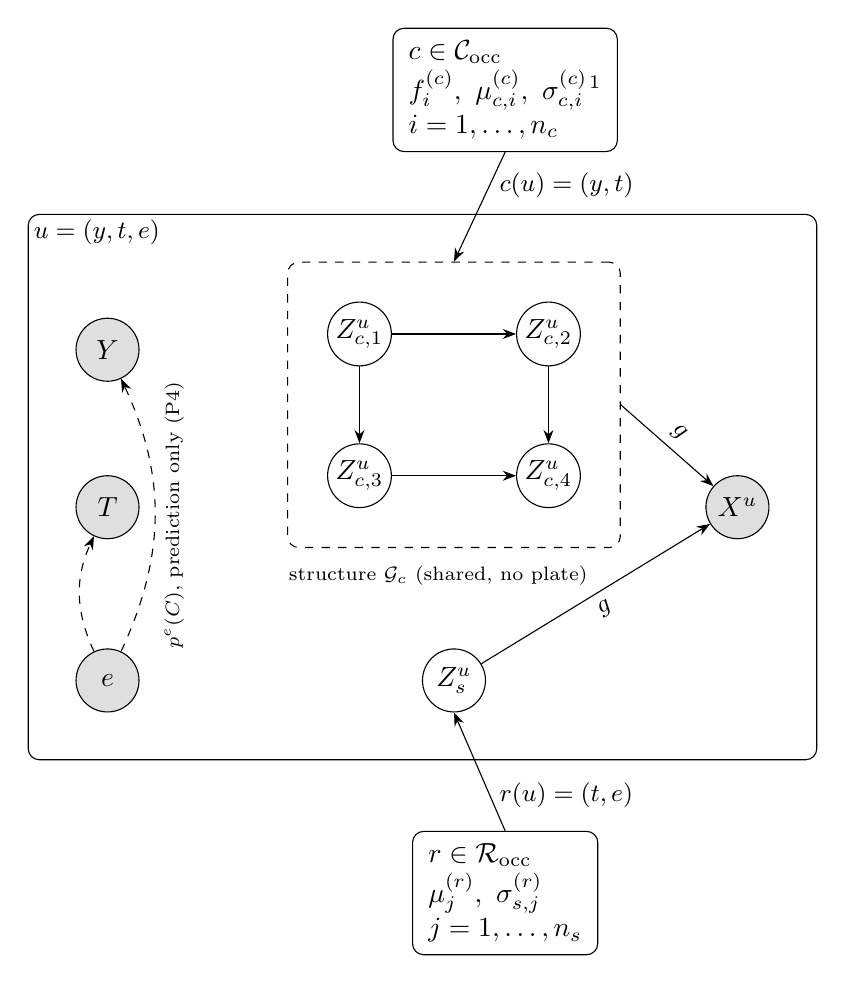
\begin{tikzpicture}[
  >=Stealth,
  node distance=8mm and 12mm,
  latnode/.style={
    circle,draw,minimum size=8mm,inner sep=1pt
  },
  obsnode/.style={
    circle,draw,fill=gray!25,minimum size=8mm,inner sep=1pt
  },
  plate/.style={
    draw,rounded corners,inner sep=4mm
  },
  platelabel/.style={font=\small,anchor=north west,inner sep=2pt},
  paramplate/.style={
    draw,
    rounded corners,
    inner xsep=2mm,
    inner ysep=1mm,
    align=left
  }
]

% ---- observed indices, inside the sample plate ----
\node[obsnode] (Y) at (-1.4,2.6) {$Y$};
\node[obsnode] (T) at (Y |- 0,0.6) {$T$};
\node[obsnode] (E) at (Y |- 0,-1.6) {$e$};

% ---- content latents (one sample's worth), with the shared DAG structure drawn once ----
\node[latnode] (c1) at (1.8,2.8)     {$Z_{c,1}^u$};
\node[latnode] (c2) at (4.2,0 |- c1) {$Z_{c,2}^u$};
\node[latnode] (c3) at (c1 |- 0,1.0) {$Z_{c,3}^u$};
\node[latnode] (c4) at (c2 |- c3)    {$Z_{c,4}^u$};

\draw[->] (c1) -- (c2);
\draw[->] (c1) -- (c3);
\draw[->] (c2) -- (c4);
\draw[->] (c3) -- (c4);

\begin{scope}[on background layer]
  \node[
    fit=(c1)(c2)(c3)(c4),
    draw,dashed,rounded corners,
    inner sep=5mm
  ] (C) {};
\end{scope}

\node[
  font=\scriptsize,
  below=1mm of C.south,
  xshift=-2mm
] {structure $\Gc$ (shared, no plate)};

\node[latnode] (s1) at (3.0,-1.6) {$Z_{s}^u$};
\node[obsnode] (X)  at (6.6,0.6)  {$X^u$};

\draw[->]
  (C.east) -- node[above,sloped,font=\small]{$g$} (X);

\draw[->]
  (s1) -- node[below,sloped,font=\small]{$g$} (X);

% ---- the sample plate: one copy per image / environment u=(y,t,e) ----
\begin{scope}[on background layer]
  \node[
    plate,
    fit=(Y)(T)(E)(C)(s1)(X),
    inner sep=6mm
  ] (plateU) {};
\end{scope}

\node[platelabel] at (plateU.north west) {$u=(y,t,e)$};

% ---- content-mechanism parameter plate: parameters indexed by the content cell c, no sample index ----
\node[
  paramplate
] (plateC) at (3.65,5.9) {%
  \begin{tabular}{@{}l@{}}
    $c\in\Cset_{\mathrm{occ}}$\\[0.1mm]
    $f_i^{(c)},\ \mu_{c,i}^{(c)},\ \sigma_{c,i}^{(c)}$\footnotemark\\[0.1mm]
    $i=1,\dots,n_c$
  \end{tabular}%
};

\draw[->]
  (plateC.south) --
  node[right,font=\small,pos=.3]{$c(u)=(y,t)$}
  (C.north);

% ---- style plate: parameters indexed by the style cell r, no sample index ----
\node[
  paramplate
] (plateR) at (3.65,-4.3) {%
  \begin{tabular}{@{}l@{}}
    $r\in\Rset_{\mathrm{occ}}$\\[0.1mm]
    $\mu_j^{(r)},\ \sigma_{s,j}^{(r)}$\\[0.1mm]
    $j=1,\dots,n_s$
  \end{tabular}%
};

\draw[->]
  (plateR.north) --
  node[right,font=\small,pos=.3]{$r(u)=(t,e)$}
  (s1.south);

% ---- P4: location-specific label prior, external to the SEM ----
\draw[->,dashed]
  (E) to[bend right=25]
  node[below,sloped,font=\scriptsize]
    {$p^e(C)$, prediction only (P4)}
  (Y);

\draw[->,dashed]
  (E) to[bend left=25]
  (T);

\end{tikzpicture}
\caption{\textbf{The M1 model, in plate notation.} The large box is the sample plate: one copy of
$(Y,T,e,Z_c^u,Z_s^u,X^u)$ per image, replicated over $u=(y,t,e)$. The two small boxes above and below
are parameter plates, replicated over the content cell $c=(y,t)$ and the style cell $r=(t,e)$
respectively; nothing inside them carries a sample index. The arrow from a parameter plate into the
sample plate is selected by that \textbf{same} image's own $(y,t)$ or $(t,e)$, as labelled (note that
$t$ is \textbf{shared}). Objects with no plate around them -- the DAG structure $\Gc$ and the mixing
$g$ -- are shared by every sample and every cell.
The dashed arrows are not part of the structural equations \eqref{eq:mixing}--\eqref{eq:style}: they
record the location-specific label prior of \labelcref{item:P4}, used only at prediction time
(\cref{sec:use}). $Y$ is unobserved and $T$ can be either observed or unobserved. The four content latents and their edges are only an illustration: the number of
content latents and their DAG are unknown.}
\label{fig:m1}
\end{figure}
\footnotetext{In an implementation, $\mu_{c,i}^{(c)}$ can be absorbed into $f_i^{(c)}$}.

\paragraph{Rationale.}
\begin{itemize}[leftmargin=1.5em]
\item \textbf{Invariance is placed where it is plausible.} Species and time of day produce animal
      appearance through a mechanism that should not depend on the camera site, so $p(z_c\mid c)$ and
      $g$ are shared across locations---\labelcref{item:P1},\labelcref{item:P2}.
\item \textbf{Locations differ by more than the label prior.} A pure shift of $p^e(C)$ (label shift)
      cannot account for differences of geography, camera and orientation. These are modelled as
      exogenous variables whose distribution depends on the location---\labelcref{item:P3}.
\item \textbf{Style depends on the time of day as well.} A specific camera and its position at a
      location may be affected in a time-of-day-specific way. The style distribution is therefore
      indexed by $(t,e)$ and not by $e$ alone. The time of day also affects the content,
      as in \labelcref{item:P2}, so it enters both
      blocks. Since $Z_s^u$ is independent of the species and of $Z_c^u$ given $(t,e)$, it carries no
      information about the species beyond what the observed $t$ already provides.
\item \textbf{Discreteness is kept in an observed variable.} $C$ is observed, so all \emph{latent}
      variables can be continuous, which is the setting of the continuous theory of
      \cite{ng2025}. No discrete-latent theory is needed.
\item \textbf{The content latents are not assumed independent.} Their DAG $\Gc$ is unknown and
      possibly non-empty; finding it is part of the problem.
\item \textbf{The number of latents is a modelling choice.} Because $C$ only indexes mechanisms,
      $n_c$ and $n_s$ are not tied to $|\Cset|$; they are hyperparameters, bounded above by the
      requirements derived in \cref{sec:reqs}.
\item \textbf{Relation to earlier frameworks.} The split into an invariant block and a changing
      block follows the partial-disentanglement idea of \cite{kong2022}; using an observed auxiliary
      variable to index changing distributions is the mechanism of \cite{khemakhem2020}. This also maps
      naturally to the application with the auxiliary variable incorporating distributions changing
      observables.
\end{itemize}


% =====================================================================
\section{The theory of Ng et al.}
\label{sec:ng}

We restate what is needed from \cite{ng2025}. For each environment $u\in[m]$ there is a latent vector
$Z^u=(Z_1^u,\dots,Z_n^u)$ and an observation $X^u=g(Z^u)$, with $g$ a $\mathrm{C}^2$ 
\textbf{\textit{diffeomorphism onto its image ((injective, smooth, smooth inverse)}}, shared by all environments. Each coordinate satisfies
$Z_i^u=f_i^{(u)}(\PA(Z_i^u;\G_Z))+\epsilon_i^{(u)}$ with $\epsilon_i^u$ Gaussian (additive noise
model, ANM; the meaning of $\epsilon_i^{(u)}$ is discussed in \cref{app:eps}), where the same unknown
DAG $\G_Z$ holds in every environment and the mechanisms $f_i^{(u)}$ may change arbitrarily with
$u$. Write $p^{(u)}_Z$ for the density of $Z^u$; it is assumed third-order differentiable (and hence 
--  continuous) with \emph{full support on $\R^{n}$}.

\subsection{Ng et al. objective}
Ng et al. objective is to learn an \textit{observationally equivalent} model 
$(\hat g, p_{\hat Z}, \hat \G_{\hat Z})$
that follows the above data generating process, and generates a data distribution that matches the 
distribution of the observed random variables $X$ across the given environments, i.e. 
(\cite[Equation 2]{ng2025}), 
\begin{equation}
p^{(u)}_{\hat X}(x) = p^{(u)}_X(x),\ \forall u \in [m],\ x \in X^{(u)},
\label{eq:obs_equiv}
\end{equation}
where $\hat Z$ denote the estimated latent variables and $\hat X = \hat{g}(\hat Z)$. In this case, 
the models $(\hat g, p_{\hat Z}, \G_{\hat Z})$ and $(g, p_Z, \G_Z)$ are said to be 
\textit{observationally equivalent}.

\subsection{Graph notions}
The \emph{Markov network} $\Mk_Z$ has an edge $\{Z_i,Z_j\}$ iff
$Z_i\not\perp Z_j\mid Z_{[n]\setminus\{i,j\}}$, equivalently iff \linebreak
$\partial^2\log p^{(u)}(Z)/\partial Z_i\partial Z_j\not\equiv0$ for some $u$; under faithfulness it is
the moral graph of $\G_Z$. Write $\mathcal{E}(\Mk_Z)$ for its edge set, $\Delta(\Mk_Z)$ for its 
set of triangles and $\deg_{\Mk_Z}(v)$ for the degree of a node. 
The \emph{surrounding parents} of $Z_i$ are
\[
\sur(Z_i;\G_Z):=\{Z_j\in\PA(Z_i;\G_Z)\mid Z_j\text{ is a parent of every child of }Z_i\}.
\]

\subsection{Sufficient-change vectors}
For a set $Z'$ of latents that contains all of its own ancestors (an \emph{ancestral} set), with
$n'=|Z'|$, let $\G_{Z'}$ be the induced DAG, $\Mk_{Z'}$ its Markov network, and define
\begin{align}
\vect\tau(Z',u) &= \Bigl(\tfrac{\partial\log p^{(u)}(Z')}{\partial Z_i}\Bigr)_{Z_i\in Z'}
\oplus\Bigl(\tfrac{\partial^2\log p^{(u)}(Z')}{\partial Z_i^2}\Bigr)_{Z_i\in Z'}
\oplus\Bigl(\tfrac{\partial^2\log p^{(u)}(Z')}{\partial Z_i\partial Z_j}\Bigr)_{\{Z_i,Z_j\}\in \mathcal{E}(\Mk_{Z'})},
\label{eq:tau}\\[2pt]
\vect w(Z',u) &= \vect\tau(Z',u)
\oplus\Bigl(\tfrac{\partial^3\log p^{(u)}(Z')}{\partial Z_i^3}\Bigr)_{Z_i\in Z'\setminus\Sk(\G_{Z'})}
\oplus\Bigl(\tfrac{\partial^3\log p^{(u)}(Z')}{\partial Z_i^2\partial Z_j}\Bigr)_{\substack{\{Z_i,Z_j\}\in \mathcal{E}(\Mk_{Z'}),\\ Z_i\notin\Sk(\G_{Z'})}} \nonumber \\
& \quad \oplus\Bigl(\tfrac{\partial^3\log p^{(u)}(Z')}{\partial Z_i\partial Z_j\partial Z_k}\Bigr)_{\{Z_i,Z_j,Z_k\}\in\Delta(\Mk_{Z'})}.
\label{eq:w}
\end{align}
In the fourth group in \cref{eq:w} we read the index set as \emph{ordered} pairs $(i,j)$: an edge contributes one entry for each endpoint that is not a sink, taking that endpoint as the squared variable. This is how
the entries arise in Eq.~(7) in the proof of Proposition~2 of \cite{ng2025}, where the sum runs over
such pairs, and how the term $3|E|$ in their count arises. (The fourth group is printed in the paper with
the index condition ``$i<j$''; see \cref{rem:ij}.)

\begin{assumption}[Sufficient changes for the Markov network, \cite{ng2025}]\label{as:1}
For every ancestral $Z'$ and every value of $Z'$ there exist $2n'+|\mathcal{E}(\Mk_{Z'})|+1$ values
$u_0,u_1,\dots$ such that the vectors $\vect\tau(Z',u_j)-\vect\tau(Z',u_0)$, $j\ge1$, are linearly
independent.
\end{assumption}

\begin{assumption}[Sufficient changes for sink nodes, \cite{ng2025}]\label{as:2}
For every ancestral $Z'$ and every value of $Z'$, with $L:=|\vect w(Z',u)|$, there exist $L+1$ values
$u_0,\dots,u_L$ such that the vectors $\vect w(Z',u_j)-\vect w(Z',u_0)$, $j=1,\dots,L$, are linearly
independent.
\end{assumption}

\begin{theorem}[Identifiability with latent ANMs, \cite{ng2025}]\label{thm:ng}
Under the data generating process above, \cref{as:1,as:2} and faithfulness, Algorithm~1 of 
\cite{ng2025}, which is required to find an \textit{observationally equivalent} model of the data
generating process, returns $(\hat{\G},\hat Z)$ such that, for some permutation $\pi$ of the estimated 
latents, (i) $\hat{\G}_\pi$ and $\G_Z$ are identical, and 
(ii) each $\hat Z_{\pi(i)}$ is solely a function of a subset of
$\{Z_i\}\cup\sur(Z_i;\G_Z)$.
\end{theorem}

The role of the third derivatives is to identify sink nodes: for a sink $Z_i$ with \textit{Gaussian}
noise, $\partial^3\log p/\partial Z_i^2\partial Z_j=0$ for all $j$ \cite{ng2025} (a property used in
score matching for observed variables in \cite{rolland2022}). With the Markov network known, the parents
of an identified sink are its neighbors; the sink is frozen and the procedure repeats on the rest.
Without further assumptions nonlinear ICA and hence CRL are not identifiable \cite{hyvarinen1999};
the environments supply the needed variation. The Markov-network stage alone is the result of
\cite{zhang2024}, which yields identification only up to mixing with ``intimate neighbors''.

Algorithm~1 requires learning $(\hat g^t, p^t_{\hat Z}, \G^t_{\hat Z})$ where $t$ is the iteration 
index under additional constraints to achieve \cref{eq:obs_equiv} -- observational equivalence. 
They propose to use a VAE to that end with additional regularization terms. 

\subsection{Gaussianity assumptions in ANM}
Ng et al. assume Gaussianity in two places: (i) In their theory exogenous noise terms and (ii) in the implementation of the VAE where all distributions that need to be specified (encoder, decoder, prior) are assumed Gaussian.

\begin{itemize}
\item \textit{In the theory}: Gaussianity of the exogenous noise is used for exactly one purpose -- the 
sink-detection property. For a sink $Z_i$ under Gaussian noise, $\log p(Z_i\mid\text{parents})$ is 
quadratic in $Z_i$, so $\partial^3\log p/\partial Z_i^2\partial Z_j=0$ for all $j$ (ANM case). This 
vanishing is what lets Algorithm~1 identify sinks via third-derivative tests and peel them off one at a 
time. It's genuinely Gaussian-specific (quadratic log-density $\Leftrightarrow$ Gaussian) -- no other 
noise family gives this cleanly. Nothing else in Assumptions~1/2 (the linear-independence conditions) 
needs Gaussianity per se; they're stated generically in terms of derivatives of $\log p^{(u)}$.

\item \textit{In the implementation}: Only one of the three Gaussian choices actually follows from the 
theory:
\begin{itemize}
\item \textbf{Prior over $\hat Z$} (\texttt{mean/logvar} nets, ANM structure) -- follows from the 
theory. This is the direct implementation of the Gaussian exogenous-noise assumption, and it's what the 
sink-freezing logic is trying to exploit (even if, per \cref{app:code}, the actual freezing rule is a 
sparsity-mask heuristic, not the literal third-derivative test).
\item \textbf{Encoder $q(z\mid x)$ Gaussian} -- does not follow from the theory. The paper says nothing 
about the recognition model's distribution; this is a standard VAE/reparameterization convenience, 
orthogonal to the noise-model assumption.
\item \textbf{Decoder Gaussian $\rightarrow$ MSE reconstruction loss} -- does not follow from the theory 
either. The paper never states a reconstruction loss at all (already noted in \cref{app:code}) as
``\textit{an implicit modelling choice not discussed in the paper}''.
This is purely a VAE-training-objective choice, not an implication of Gaussian noise in the SEM.
\end{itemize}
So: theory constrains the prior; encoder and decoder Gaussianity are independent engineering choices 
riding along with ``\textit{it's a VAE}'', not consequences of the identifiability assumption.
\end{itemize}

\subsection{Gaussianity assumptions in HNM}
\begin{itemize}
\item \textit{Theory}: Gaussianity still does exactly the same job -- identifying sinks -- but the 
property it buys is weaker. Now $\epsilon_i\sim\mathcal N(0,1)$ and the scale $\sigma_i^{(u)}(\PA(Z_i))$ 
carries the parent-dependence, so $\log p(Z_i\mid\PA)$ is no longer purely quadratic in $Z_i$ 
(the $\log\sigma_i(\PA)$ term depends on the parents too). Result: $\partial^3\log p/\partial 
Z_i^2\partial Z_j=0$ only for $Z_j\notin\PA(Z_i)$ -- vanishes for non-parents, not for parents. So 
Gaussianity of $\epsilon_i$ is still what makes the non-parent third derivatives vanish; it just no 
longer kills the parent ones, because the heteroscedastic scale reintroduces parent-dependence into the 
third derivative.

Practically this means the sink test still works, but is less informative: you learn 
\textit{``no non-parent neighbors act on $Z_i$ nontrivially,}'' but you don't get the same clean 
``\textit{this column of the adjacency is zero}'' signal from the pure log-density curvature -- you 
still need the Markov network (second derivatives) to know who the candidate neighbors are, and the 
third-derivative sink test now only rules out non-parents rather than certifying the full parent set 
directly the way it did in the ANM.
\newpage
\item \textit{Implementation}:
\begin{itemize}
\item \textbf{Prior} -- same story, just needs \texttt{log\_var\_net} (or whatever computes 
$\hat\sigma_i^{(u)}$) to also take the masked/estimated parents as input, not just $u$. Still 
{theory-driven}.
\item \textbf{Encoder/decoder Gaussianity} -- unaffected, same VAE convenience as before, orthogonal to 
ANM vs. HNM.
\item \textbf{Sink-freezing heuristic} (\texttt{find\_sinknodes\_and\_fix}) -- 
this one actually gets harder to 
justify under HNM, since the mask-based heuristic was already a loose proxy for the ANM's sharp third-
derivative test; under HNM the thing it's supposed to approximate is itself weaker, so the gap between 
``\textit{heuristic zeros out a column}'' and ``\textit{theorem's sink property}'' widens rather than 
narrows.
\end{itemize}
\end{itemize}

% =====================================================================
\section{M1 inside the framework of Ng et al.}
\label{sec:apply}

\subsection{Environments}
An environment is a triple $u=(c,e)=(y,t,e)$; its observed distribution is
$p^{(u)}(x)=p(x\mid y,t,e)$, which is available because all three indices are observed. In this
indexing
\begin{center}
\begin{tabular}{@{}lll@{}}
\toprule
latent block & \shortstack[l]{depends on $u=(y,t,e)$\\only through} & mechanism\\
\midrule
content $Z_c$ & $c=(y,t)$ & $f_i^{(c)},\ \sigma_{c,i}^{(c)}$ (soft changes of an unknown DAG)\\
style $Z_s$ & $r=(t,e)$ & $\mu_j^{(r)},\ \sigma_{s,j}^{(r)}$ (isolated nodes)\\
\bottomrule
\end{tabular}
\end{center}
so M1 is an instance of the process in \cref{sec:ng} with a particular pattern of which mechanisms
change: the same DAG $\G=\Gc\,\cup\,\{\text{isolated nodes}\}$ in all environments, Gaussian noise for
every latent, and $g$ shared.

\subsection{Block structure of the sufficient-change vectors}
Given $u=(y,t,e)$,
\[
\log p^{(u)}(z)=\log p(z_c\mid c)+\sum_{j=1}^{n_s}\log p^{(r)}(z_{s,j}),\qquad c=(y,t),\ r=(t,e).
\]
Hence all cross derivatives between the blocks vanish, the Markov network is $\Mk_c$ (the network of
$\Gc$) plus isolated nodes, and every ancestral set is $Z'=Z'_c\cup Z'_s$. The vector splits:
\begin{equation}
\vect w(Z',u)=\bigl(\vect w_c(Z'_c,c),\ \vect b(Z'_s,r)\bigr),
\qquad \vect b(Z'_s,r)=\Bigl(\tfrac{\partial\log p^{(r)}(z_{s,j})}{\partial z_{s,j}},
\tfrac{\partial^2\log p^{(r)}(z_{s,j})}{\partial z_{s,j}^2}\Bigr)_{j}.
\label{eq:split}
\end{equation}
An isolated node is a sink with no edges. It is excluded from every third-order group of
\cref{eq:w}, so a style latent contributes exactly two entries, its first and second derivative. If
all style latents are in $Z'$, then $|\vect b|=2n_s$. The two blocks are functions of different parts of $u$,
but both depend on the time of day: $\vect w_c$ on $c=(y,t)$ and $\vect b$ on $r=(t,e)$.

\subsection{What \texorpdfstring{\cref{thm:ng}}{Theorem~\ref*{thm:ng}} of Ng et al. gives for M1}
The graph $\G$ is recovered up to isomorphism. Every style latent has no parents, hence \linebreak
\mbox{$\sur(Z_{s,j};\G)=\varnothing$}, so each estimated style latent is a component-wise (invertible)
function of one true style latent. Every content latent is a function of itself and its surrounding
parents, all of which lie in the content block. Consequently:
\begin{center}
\fbox{\emph{no estimated latent mixes content and style.}}
\end{center}
This is the property that makes transfer to an unseen location possible (see \cref{sec:use}).
Note that what partial disentanglement (nonempty $\sur(Z_i)$) actually costs you is in interpretability 
of individual latents (you can't point to ``this coordinate = leg length''), not predictive usability. 
The content/style split is the property you need for prediction to work at all (style drops out), and 
that one is clean regardless of $\sur(Z_i)$ (see \cref{sec:apply}).

\subsection{Requirements on the environments}
\label{sec:reqs}
Let $L_c$ be the number of entries of $\vect w_c$ for the full content block, computed in
\cref{prop:count} below, and $L_s=2n_s$.

\begin{proposition}[Requirements for M1]\label{prop:m1req}
Fix a value of $Z=(z_c,z_s)$ and suppose \cref{as:2} holds for $Z'=Z$ at this value. Write
$\vect a(c)=\vect w_c(z_c,c)\in\R^{L_c}$ and $\vect b(r)=\vect b(z_s,r)\in\R^{L_s}$. For an occurring
environment $u=(y,t,e)$ the vector is $\vect w(u)=(\vect a(y,t),\vect b(t,e))$. Then
\begin{enumerate}[label=(\alph*),leftmargin=2em]
\item \label{item:Lc} $L_c\ \le\ K_C-1$;
\item \label{item:Ls} $L_s=2n_s\ \le\ K_R-1$;
\item \label{item:Lc+Ls} $L_c+L_s\ \le\ \sum_{t\in\Tset_{\mathrm{occ}}}\bigl(|\Yset_t|+|\Lset_t|-2\bigr)+|\Tset_{\mathrm{occ}}|-1$.
\end{enumerate}
\end{proposition}

\begin{proof}
Let $V$ be the linear span of the differences $\vect w(u)-\vect w(u_0)$ over occurring environments, i.e.\
the direction space of the affine hull $H$ of the points $\vect w(u)$. \Cref{as:2} requires
$\dim V=L_c+L_s$; in particular the projection of $V$ onto each block must be onto.
\labelcref{item:Lc} The projection onto the content block is the direction space of the affine hull of the $K_C$ points
$\vect a(c)$, of dimension at most $K_C-1$; it must equal $\R^{L_c}$.
\labelcref{item:Ls} Likewise the projection onto the style block is spanned by differences of the $K_R$ points $\vect b(r)$.
\labelcref{item:Lc+Ls} For each $t$, the points with time of day $t$ lie in the product of the affine hull of
$\{\vect a(y,t)\}_{y\in\Yset_t}$ and the affine hull of $\{\vect b(t,e)\}_{e\in\Lset_t}$, an affine subspace $F_t$
of dimension at most $(|\Yset_t|-1)+(|\Lset_t|-1)$. The hull $H$ is contained in the affine hull of
$\bigcup_t F_t$, whose dimension is at most $\sum_t\dim F_t+|\Tset_{\mathrm{occ}}|-1$ (the affine hull of $k$
affine subspaces has dimension at most the sum of their dimensions plus $k-1$). Hence
$L_c+L_s=\dim V\le\sum_t(|\Yset_t|+|\Lset_t|-2)+|\Tset_{\mathrm{occ}}|-1$.
\end{proof}

\begin{remark}[Sufficiency]\label{rem:suff}
The inequalities are necessary for \cref{as:2}. If every combination $(y,t,e)$ occurs and the vectors are in
general position subject to the block structure, they are also sufficient, for the following reason. The
within-$t$ differences supply up to $\sum_t(|\Yset_t|-1)$ independent directions in the content block and up
to $\sum_t(|\Lset_t|-1)$ in the style block, and each of the $|\Tset_{\mathrm{occ}}|-1$ differences across
times of day adds one further direction that moves \emph{both} blocks at once. I do not prove general
position for the actual vectors, which are constrained by the Gaussian form of the model, so sufficiency is
expected but not established. The coupling through $T$ is the reason for \labelcref{item:Lc+Ls}: the
extra directions from changing $T$ are shared between the two blocks and cannot be counted twice.
\end{remark}

\begin{example}[Numbers for the camera-trap data]\label{ex:numbers}
Suppose the ten species are combined with a binary time of day, all combinations occur, and the three
training locations each see both times of day. Then $K_C=20$, $K_R=6$ and the bound in
\labelcref{item:Lc+Ls} equals
$2(10+3-2)+1=23$. Condition \labelcref{item:Lc} gives $L_c\le19$.
Condition \labelcref{item:Ls} gives $2n_s\le5$, hence $n_s\le2$, so
$L_s\le4$.
Then \labelcref{item:Lc+Ls} never binds beyond \labelcref{item:Lc}, because $19+4=23$.
If the style distribution depended on the
location only, as in an earlier version of M1, then $K_R$ would be $3$ and $n_s\le1$.
\end{example}

\Cref{as:2} must hold at every value of $Z$ and for every ancestral $Z'$; the proposition addresses the
whole set $Z'=Z$ at one value and is the natural binding case, but we do not claim that no other ancestral set
is more demanding.

\begin{proposition}[Entry count]\label{prop:count}
For an ancestral set $Z'$ with $n'$ nodes, $E=|\mathcal{E}(\Mk_{Z'})|$ edges and $D=|\Delta(\Mk_{Z'})|$
triangles in its Markov network, and sink set $\Sk=\Sk(\G_{Z'})$,
\begin{equation}
L=|\vect w(Z',u)|=3n'+3E+D-|\Sk|-\sum_{v\in\Sk}\deg_{\Mk_{Z'}}(v).
\label{eq:L}
\end{equation}
\end{proposition}

\begin{proof}
The groups of \cref{eq:w} have sizes: $n'$ (first derivatives), $n'$ (pure second), $E$ (mixed
second), $n'-|\Sk|$ (pure third, non-sinks), $\sum_{i\notin\Sk}\deg(i)=2E-\sum_{v\in\Sk}\deg(v)$ (mixed
third, one entry per non-sink endpoint of each edge) and $D$ (triple). Adding gives \cref{eq:L}.
\end{proof}

For the content block use \cref{eq:L} with $Z'=Z_c$ to get $L_c$. \Cref{tab:examples} lists
$L_c$ for some content graphs, and what fits into the $K_C=20$ values available under the assumptions of
\cref{ex:numbers}.

\begin{table}[ht]
\centering
\caption{Content-block requirement $L_c$ from \cref{eq:L}; condition \labelcref{item:Lc} of
\cref{prop:m1req} is $K_C\ge L_c+1$, i.e.\ $L_c\le 19$ for $K_C=20$.}
\label{tab:examples}
\begin{tabular}{@{}lccccccc@{}}
\toprule
content graph $\Gc$ & $n_c$ & $E$ & $D$ & sinks (degree) & $L_c$ & $L_c+1$ & fits $K_C{=}20$?\\
\midrule
empty                              & 9 & 0 & 0 & 9 (all 0) & 18 & 19 & yes\\
empty                              & 10 & 0 & 0 & 10 (all 0) & 20 & 21 & no\\
collider $Z_1\to Z_2\leftarrow Z_3$ & 3 & 3 & 1 & 1 (deg.\ 2) & 16 & 17 & yes\\
chain, 3 nodes                     & 3 & 2 & 0 & 1 (deg.\ 1) & 13 & 14 & yes\\
chain, 4 nodes                     & 4 & 3 & 0 & 1 (deg.\ 1) & 19 & 20 & yes (barely)\\
chain, 5 nodes                     & 5 & 4 & 0 & 1 (deg.\ 1) & 25 & 26 & no\\
\bottomrule
\end{tabular}
\end{table}

For the style block with Gaussian noise, $\log p^{(r)}(z_{s,j})=-(z_{s,j}-\mu_j^{(r)})^2/(2(\sigma_{s,j}^{(r)})^2)+\text{const}$, so
\[
\vect b(z_s,r)=\Bigl(\tfrac{\mu_j^{(r)}}{(\sigma_{s,j}^{(r)})^2}-\tfrac{z_{s,j}}{(\sigma_{s,j}^{(r)})^2},\
-\tfrac1{(\sigma_{s,j}^{(r)})^2}\Bigr)_{j=1,\dots,n_s}.
\]
For fixed $z_s$ this is an invertible affine function of the natural parameters
$\bigl(\mu_j^{(r)}/(\sigma_{s,j}^{(r)})^2,\,1/(\sigma_{s,j}^{(r)})^2\bigr)_j$. Hence the requirement that the
$K_R$ points $\vect b(r)$ affinely span $\R^{2n_s}$ is the requirement that the natural-parameter vectors
over the style cells $(t,e)$ affinely span $\R^{2n_s}$. For $n_s=1$ this means that the points
$(\mu^{(r)}/(\sigma^{(r)})^2,\,1/(\sigma^{(r)})^2)$ over the cells are not all collinear. A pure shift of the
mean, with equal variances in all cells, puts them on a line and violates the requirement.

\begin{remark}
These are conditions of the proof technique of \cite{ng2025}, and identification can be possible with
less. \Cref{prop:m1req} states necessary conditions for \cref{as:2}; sufficiency is discussed in
\cref{rem:suff}. For M1 under the assumptions of \cref{ex:numbers}, the bounds allow up to nine content
latents if $\Gc$ is empty, correspondingly fewer for denser $\Gc$, and at most two style latents.
\end{remark}


% =====================================================================
\section{The environment count: paper's formula vs the definition}
\label{sec:count}

Ng et al.\ state that the number of environments needed is (at least) 
\cite[subsection ``Number of environments'']{ng2025}
\begin{equation}
N_{\mathrm{paper}}=3n+3|\mathcal{E}(\Mk_Z)|+|\Delta(\Mk_Z)|-2|\Sk(\G_Z)|+1 .
\label{eq:paper}
\end{equation}
\Cref{as:2} asks for $L+1$ values of $u$, with $L$ the length of $\vect w$. Counting the entries of
\cref{eq:w} directly gives \cref{eq:L}, hence a requirement of $L+1$ environments, and
\begin{equation}
N_{\mathrm{paper}}-(L+1)=\sum_{v\in\Sk(\G_Z)}\bigl(\deg_{\Mk_Z}(v)-1\bigr).
\label{eq:diff}
\end{equation}
So the formula in the paper agrees with the count from the definition exactly when the total degree of the
sinks in the Markov network equals the number of sinks; in particular this holds when every sink has
exactly one edge. Otherwise the two differ by one for each unit of excess degree of a sink (positive
difference) or for each isolated sink (negative difference).

\begin{table}[ht]
\centering
\caption{Count according to formula in \cref{eq:paper} versus the count $L+1$ from the definition of $\vect w$.}
\label{tab:paper}
\begin{tabular}{@{}lccccc@{}}
\toprule
graph & $n$ & sinks (degree) & $L$ & $L+1$ & $N_{\mathrm{paper}}$\\
\midrule
single isolated node                 & 1 & 1 (0) & 2  & 3  & 2 \\
chain $Z_1\to Z_2\to Z_3$             & 3 & 1 (1) & 13 & 14 & 14\\
collider $Z_1\to Z_2\leftarrow Z_3$   & 3 & 1 (2) & 16 & 17 & 18\\
empty graph on $n$ nodes              & $n$ & $n$ (all 0) & $2n$ & $2n+1$ & $n+1$\\
\bottomrule
\end{tabular}
\end{table}

As a sanity check, $\vect w$ contains $\vect\tau$, so \cref{as:2} needs at least the
$2n+|E|+1$ environments of \cref{as:1}. For the empty graph the printed formula gives $n+1<2n+1$,
which cannot be right; the formula appears to presuppose that sinks have exactly one Markov-network
edge (for instance, leaf nodes with one parent). I could not find a derivation of \cref{eq:paper} in
the text; it is stated as a lower bound. For M1 the difference matters because the style latents are
isolated sinks: the definition gives two entries for each (as in \cref{eq:split}), whereas
\cref{eq:paper} would charge only one. We therefore use the count from the definition.

\begin{remark}[Reading of the index set]\label{rem:ij}
The fourth group of $\vect w$ is printed in \cite{ng2025} with the index condition ``$i<j$,
$\{Z_i,Z_j\}\in\mathcal{E}(\Mk_{Z'})$, $Z_i\notin\Sk(\G_{Z'})$''. Read literally this depends on how the nodes are
indexed. The paper states that Algorithm~1 outputs the estimated latents in a causal order, and its proof
of Theorem~1 uses a causal order of the true latents. With indices in a causal order the literal reading
is well defined. For an edge of the Markov network (the moral graph) the lower-indexed endpoint is either
the parent in a parent--child edge or a co-parent of a later common child; in both cases it has a child,
so it is never a sink and the condition $Z_i\notin\Sk$ is redundant. Each edge then contributes exactly
one entry, $\partial^3\log p/\partial Z_i^2\partial Z_j$ with $i<j$. I do not think this is the intended
set, for two reasons.
\begin{enumerate}[label=(\roman*),leftmargin=2em]
\item Eq.~(7) in the proof of Proposition~2 of \cite{ng2025} contains a term with squared variable
      $Z_{\alpha(i)}$ for \emph{every} ordered pair $(i,j)$ of adjacent nodes with $Z_{\alpha(i)}$ a non-sink;
      unlike the neighbouring second-order and triple sums, it has no ``$i<j$''. If both endpoints of an
      edge are non-sinks, the monomials $(\partial Z_i/\partial\hat Z_l)^2\,\partial Z_j/\partial\hat Z_l$ and
      $(\partial Z_j/\partial\hat Z_l)^2\,\partial Z_i/\partial\hat Z_l$ have separate coefficients. The
      argument that each coefficient vanishes rests on the linear independence in \cref{as:2}, so
      both derivatives must be entries of $\vect w$.
\item With one entry per edge the length is $L=3n+2|E|+|\Delta|-|\Sk|$, so the number of environments
      $L+1$ would be $13$ for the chain and $16$ for the collider of \cref{tab:paper}, against $14$ and $18$
      in the printed formula \cref{eq:paper}. Ordered pairs give $14$ and $17$, matching the printed
      formula for the chain.
\end{enumerate}
I therefore keep ordered pairs and read the ``$i<j$'' in the fourth group as a notational slip. This is my
reading, not a statement in the paper.
\end{remark}

% =====================================================================
\section{Estimation and use at an unseen location}
\label{sec:use}

\paragraph{Prediction at an unseen location.}
Algorithm~1 of \cite{ng2025} applies with environments $u=(y,t,e)$. A VAE with a shared encoder and
decoder is trained on all environments. The prior over $\hat Z_c$ is a Gaussian ANM whose mechanism
parameters are conditioned on $c=(y,t)$ (for instance through embeddings of $y$ and $t$), and the prior over
$\hat Z_s$ has mean and variance conditioned on $r=(t,e)$. The adjacency matrix of the content block is learned
with the sparsity and moral-graph penalties of \cite{ng2025}, and sinks are identified and frozen
iteratively. The style coordinates may be designated in advance as isolated nodes or discovered as estimated
nodes with no edges whose distribution depends on $(t,e)$ but not on the species $y$; an isolated content
latent with no parents whose distribution depends on $y$ is a content latent. The numbers of latents $n_c$
and $n_s$ are hyperparameters; \cite{ng2025} suggest choosing the number of latents by the ELBO.
(\Cref{app:code} documents, against the released reference code, which of these pieces are already
implemented, which are only partly implemented, and which still need to be built for M1.)

\paragraph{Prediction at a new location $e^\ast$.}
Encode $x$ to $(\hat z_c,\hat z_s)$. Since $x\leftrightarrow(z_c,z_s)$ is an injection, the 
posterior of $C=(Y,T)$ is
$$
p(c\mid x^\ast,e^\ast) = p(c\mid z_c,z_s,e^\ast) = p(y,t\mid z_c,z_s,e^\ast) =
p(y\mid t,z_c,z_s,e^\ast)p(t\mid z_c,z_s,e^\ast).
$$
Two cases exist: Time of day observed or unobserved at test time.
\begin{itemize}
\item \emph{Time of day observed at test time.} Since $Z_s$ is independent of $(Y,Z_c)$
	given $(x^\ast,t^\ast,e^\ast)$,
	\begin{equation}
	p(y\mid x^\ast,t^\ast,e^\ast) =
	p(y\mid z_c,z_s,t^\ast,e^\ast) =
	p(y\mid z_c,t,e^\ast)\ \propto\ p^{e^\ast}(y\mid t^\ast)\,p(z_c\mid y,t^\ast),
	\label{eq:predict}
	\end{equation}
	so the style latents drop out exactly and only the content latents are used.
	Hence, the species $y$ can be inferred from maximizing the likelihood-prior product over $y$ for 
	the given $t^\ast$.
	The factor $p(z_c\mid y,t^\ast)$ is invariant by \labelcref{item:P2}.
	The prior $p^{e^\ast}(y\mid t^\ast)$ can be obtained from the location-specific prior 
	$p^{e^\ast}(C)$;
	it can be taken equal to the pooled training prior, or estimated from unlabeled images of 
	$e^\ast$ (for
	instance by EM), if multiple images are available, or assumed to be uniform and ignored. No 
	style parameters of $e^\ast$ are needed.

\item \emph{Time of day not observed.} Then
	$p(c\mid z_c,z_s,e^\ast)\propto p^{e^\ast}(c)\,p(z_c\mid c)\,p^{(t,e^\ast)}(z_s)$, and the last 
	factor depends on $t$, so the style carries information about the time of day. Dropping it gives
	$p(c\mid z_c,e^\ast)\propto p^{e^\ast}(c)\,p(z_c\mid c)$, which is the correct posterior given 
	$z_c$
	alone but not the full posterior; using the style would require the style distributions of the 
	new  location for each time of day, which are not available from labelled data.

	Coarse time of day could be approximated by the image's brightness:
	This is reasonable, with one caveat. Brightness is mostly determined by style (exposure, IR 
	mode) and by $t$, so it works as a cheap, fixed read-out of part of $z_s$. It fails if a new 
	camera shifts the day/night threshold, for example a flash-lit night image or a shaded day 
	image.

	We can measure this before relying on it. Fit brightness $\rightarrow$ day/night on some on the 
	training locations and test on the rest. Then there are two cases:
	\begin{enumerate}
	\item If the error is near zero, treat $t$ as observed and use
		$p(y \mid z_c, t) \ \propto\ \bar{p}(y|\tilde{t})p(z_c \mid y,\tilde{t})$, where $\tilde{t}$ 
		is the estimated $t$ from brightness.
	\item If not, use it softly:
		$p(y \mid z_c, b) \ \propto\ \sum_t \bar{p}(y,t)p(z_c \mid y,t)p(b \mid t)$.
		This assumes brightness $b$ depends on the image only through $t$ and style, not on the 
		species content, which holds roughly unless animal coat color moves overall brightness.

		The soft version still needs $p(b \mid t)$ at L100, which you take from the pooled training 
		data. That is the same unknown style distribution as before, but one-dimensional, so a rough 
		version is far more benign than the full style vector.
\end{enumerate}
\end{itemize}


% =====================================================================
\section{VAE architecture for M1: end-to-end vs.\ split backbone+head}
\label{sec:arch}

\Cref{sec:use} sketches the M1 prior and loss abstractly, on top of whatever encoder/decoder
produces $\hat Z$ from $X$. \Cref{thm:ng} and the propositions built on it in this note are stated for
exactly one generative object: $X=g(Z)$, with $X$ the actual observed image and $g$ the true, unknown
mixing map. Only one of the two architectures compared in this section actually instantiates that
object. \Cref{sec:archA} (end-to-end) does. \Cref{sec:archB} (split, frozen backbone) does not: it
reconstructs a backbone-derived quantity, not $X$, and nothing in \cite{ng2025} says anything about the
resulting model (\cref{sec:archB:gap}). \Cref{sec:archB} is kept in this note anyway, but as what it
is -- an unproven speed heuristic, not a second way of applying the theory -- and this section is
written to say so plainly rather than to imply otherwise. \Cref{app:code} is used throughout as the
concrete description of what the reference implementation of Ng et al. \cite{ngimpl} already provides
and what it is missing.

\subsection[Option A: end-to-end]{Option A: end-to-end -- the only option that implements \cref{def:m1} and \cref{thm:ng} as stated}
\label{sec:archA}
The backbone and the VAE head are one model, trained jointly on raw $224\times224$ images: a
ResNet-50 feeds \texttt{encoder\_mu}/\texttt{encoder\_logvar}, and every term of the M1 loss
(reconstruction, KL, sparsity; \cref{app:code} on \texttt{Trainer.step}) backpropagates through the
head \emph{and} through the backbone. This is the only one of the two options in which the object
being reconstructed -- and hence the object the identifiability argument is actually about -- is the
true image $x$: the composite (backbone $+$ head) plays the role of the encoder, its decoder plays the
role of $g$, and the loss compares $\hat x$ against the actual $x$, exactly $X=g(Z)$ of \cref{def:m1},
with no intermediate object substituted in. \Cref{fig:optA} shows the flow.

\begin{figure}[H]
\centering
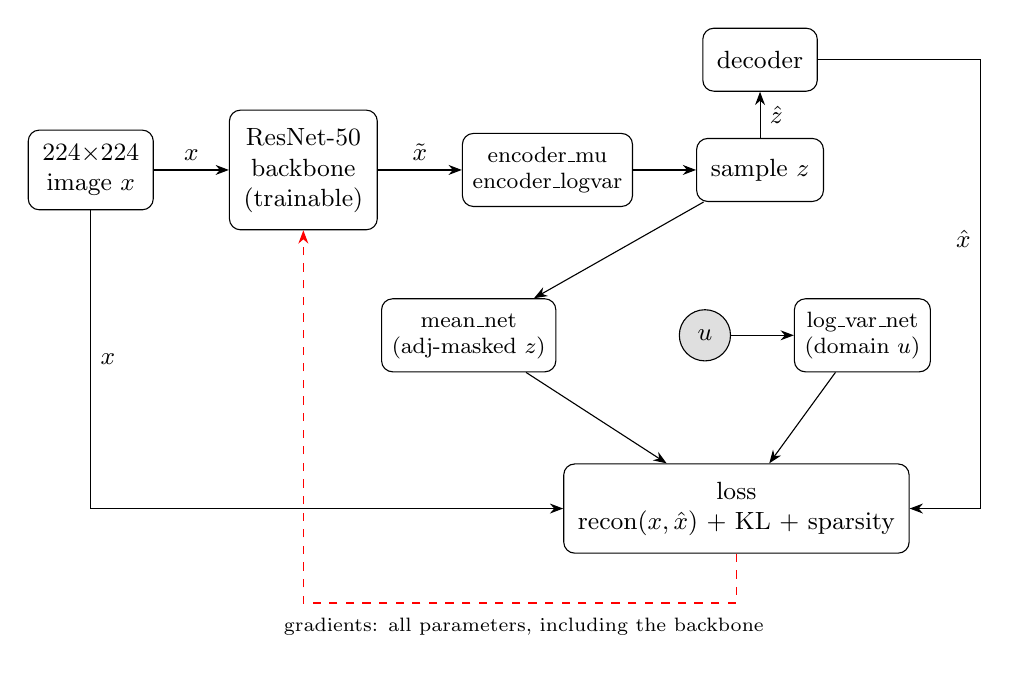
\begin{tikzpicture}[
  >=Stealth,
  font=\small,
  procnode/.style={draw,rounded corners,align=center,inner sep=1.8mm,minimum height=8mm},
  smallnode/.style={draw,rounded corners,align=center,inner sep=1.3mm,font=\footnotesize,minimum height=7mm},
  obsnode/.style={circle,draw,fill=gray!25,minimum size=6.5mm,inner sep=1pt}
]

\node[procnode] (img) at (0.8,3) {224$\times$224\\image $x$};
\node[procnode] (bb) at (3.5,0 |- img.east) {%
  \begin{tabular}{@{}c@{}} ResNet-50 \\ backbone \\ (trainable) \end{tabular}};
\node[smallnode] (enc) at (6.6,0 |- bb.east) {%
  \begin{tabular}{@{}c@{}} encoder\_mu \\ encoder\_logvar \end{tabular}};
\node[procnode] (z) at (9.3,0 |- enc.east) {sample $z$};
\node[procnode] (dec) at (0.3,4.4 -| z.north) {decoder};
%\node[procnode] (xhat) at (12.1,0 |- dec.east) {$\hat x$};

\node[smallnode] (meannet) at (5.6,0.9) {%
  \begin{tabular}{@{}c@{}} mean\_net \\ (adj-masked $z$) \end{tabular}};
\node[obsnode] (u) at (8.6,0 |- meannet.east) {$u$};
\node[smallnode] (logvarnet) at (10.6,0 |- u.east) {%
  \begin{tabular}{@{}c@{}} log\_var\_net \\ (domain $u$) \end{tabular}};

\node[procnode] (loss) at (9.0,-1.3) {%
  \begin{tabular}{@{}c@{}} loss \\ recon$(x,\hat x)$ + KL + sparsity \end{tabular}};

\draw[->] (img) -- node[above] {$x$} (bb);
\draw[->] (bb) -- node[above] {$\tilde x$} (enc);
\draw[->] (enc) -- (z);
\draw[->] (z) -- node[right] {$\hat z$} (dec);
%\draw[->] (dec) -- (xhat);
\draw[->] (z) -- (meannet);
\draw[->] (u) -- (logvarnet);
\draw[->] (meannet) -- (loss);
\draw[->] (logvarnet) -- (loss);

\coordinate (dropX1) at (12.1,0 |- dec.east);
\coordinate (dropX2) at (dropX1 |- loss);

\draw[->]
  (dec) -- (dropX1)
  -- node[left,pos=.4] {$\hat x$}
  (dropX2)
  -- (loss);

\coordinate (dropA1) at (loss.south |- 0,-2.5);
\coordinate (dropA2) at (dropA1.west -| 3.5,0);
\draw[->,dashed,red] (loss.south) -- (dropA1) -- (dropA2) -- (bb.south);
\node[font=\scriptsize,align=center] at (6.3,-2.8)
  {gradients: all parameters, including the backbone};

\coordinate (dropI1) at (img.south |- loss.west);
\draw[->]
  (img.south)
    -- node[right,midway] {$x$}
  (dropI1)
    -- (loss.west);

\end{tikzpicture}
\caption{\textbf{\nameref{sec:archA}} Every training step runs the full backbone forward, and the
M1 loss (dashed red) backpropagates through the VAE head and through the backbone. The reconstruction
term compares $\hat x$ against the true image $x$ -- the object \cref{def:m1,thm:ng} are stated about.}
\label{fig:optA}
\end{figure}
\newpage
\subsection[Option B: split]{Option B: split (frozen backbone, cached features) -- a heuristic, not a
second implementation of the theory}
\label{sec:archB}
Three separate stages: one to adapt the backbone, one (also run only once) to extract and cache
features, and one -- the actual M1 estimation -- that is trained and re-trained many times as the
prior/graph design is iterated. Write $x$ for the true image and $\tilde x:=\mathrm{BB}(x)$ for the
backbone's output, cached at stage 2 (the $\sim\!3000$-dim embedding described below). This notation
matters: as \cref{sec:archB:gap} makes precise, stage 3 never sees $x$ at all, only $\tilde x$, and
everything below should be read with that substitution in view.
\begin{enumerate}[label=(\arabic*),leftmargin=2em]
\item \textbf{Backbone adaptation (once).} Start from an ImageNet-pretrained ResNet-50. Adjust only its
      batch-norm (BN) layers to TerraIncognita (TI); every other weight stays frozen. 
      Concretely: run the network in
      \texttt{train()} mode (so BN layers update from batch statistics) but with gradients disabled,
      over batches pooled across the three training locations L38/L43/L46 (never L100), with BN 
      momentum set to \texttt{None} so each layer's running mean/variance is a cumulative 
      (equally-weighted) average of the per-batch statistics over the whole pass, rather than an 
      exponential moving average dominated by recent batches.
\item \textbf{Feature extraction (once).} Run the BN-adjusted, still-frozen backbone $\mathrm{BB}$ in
      \texttt{eval()} mode once over every image $x$ -- train and test, L100 included -- and cache
      $\tilde x=\mathrm{BB}(x)$ (per the settled pipeline: layer3 pooled concatenated with the final
      pooled layer, plus a brightness scalar) together with species/location/time-of-day/image-id in
      one table. This pass never touches a gradient and never needs to be repeated once the backbone
      from step (1) is fixed.
      \begin{itemize}
      \item \texttt{layer3} refers to ResNet-50's third residual stage 
      For a 224$\times$224 input:
      \begin{itemize} 
      \item \texttt{layer3} output: 1024 channels, 14$\times$14 spatial
	      $\rightarrow$ global-average-pooled to a 1024-dim vector
      \item \texttt{layer4} output (the ``final" stage before the classifier): 2048 channels, 7$\times$7 
	      spatial $\rightarrow$ pooled to 2048-dim -- this is the standard ``ResNet-50 feature vector"
	  \end{itemize}      
      Concatenating the two gives $\sim$3072 dims total, i.e.\ $\tilde x\in\R^{3072}$. The reason to
      include \texttt{layer3} and not just the usual final-layer 2048-dim vector: \texttt{layer4} 
      sits right before the (originally) 1000-way ImageNet classifier, so it's the most abstracted, 
      most class- \linebreak
      discriminative, and the stage most likely to have had low-level nuisance 
      information (illumination, color balance, camera signature) trained \textit{out} of it. 
      \texttt{layer3} 
      is one stage earlier and less abstracted, so it retains more texture/color/illumination 
      detail -- the kind of signal the M1 style block needs. Concatenating both gives one embedding 
      that's more likely to carry both content-relevant and style-relevant information, rather than 
      betting everything on whichever the last layer kept.
      \item \textit{Brightness} scalar: mean luminance of the image, computed as a plain scalar, not 
      from the network at all. Concretely:
      \begin{itemize}
      \item convert the image to luminance via a standard weighted sum, 
       		e.g. $Y = 0.299R + 0.587G + 0.114B$ (or BT.709 weights $0.2126/0.7152/0.0722$ -- either is 
       		fine, just stay consistent) 
      \item average $Y$ over all pixels $\rightarrow$ one number per image
      \end{itemize}
      Important detail: compute this on the raw resized image (pixel values in their normal range, e.g. 
      $[0,255]$ or $[0,1]$), before ImageNet mean/std normalization -- normalizing per-channel with 
      ImageNet's statistics would distort the brightness value in a way tied to ImageNet's own color 
      statistics, not the image's actual brightness. Same measure must be used at train and test time 
      (including on L100), since the note later proposes brightness as a TOD proxy -- consistency there 
      matters more than the exact formula chosen.
      \end{itemize}
\item \textbf{M1 estimation (iterated many times).} The M1 VAE (the small MLPs of \cref{app:code},
      modified per \cref{sec:use}) is trained on the cached tensor dataset $\tilde x$ from step (2);
      only those MLPs ever receive a gradient, and none of it touches the backbone. Its encoder maps
      $\tilde x\mapsto\hat Z$, and its decoder maps $\hat Z\mapsto\hat{\tilde x}$ -- a reconstruction of
      the cached embedding, not of the image. The reconstruction term of the loss is therefore
      $\mathrm{recon}(\tilde x,\hat{\tilde x})$, not $\mathrm{recon}(x,\hat x)$; \cref{fig:optB} draws
      this explicitly. This is the step that is actually redesigned and re-run repeatedly --
      content/style $u$-dependence, ANM vs.\ HNM, the sink-freezing rule -- while steps (1) and (2)
      stay fixed.
\end{enumerate}
\Cref{fig:optB} shows the flow.

\begin{figure}[H]
\centering
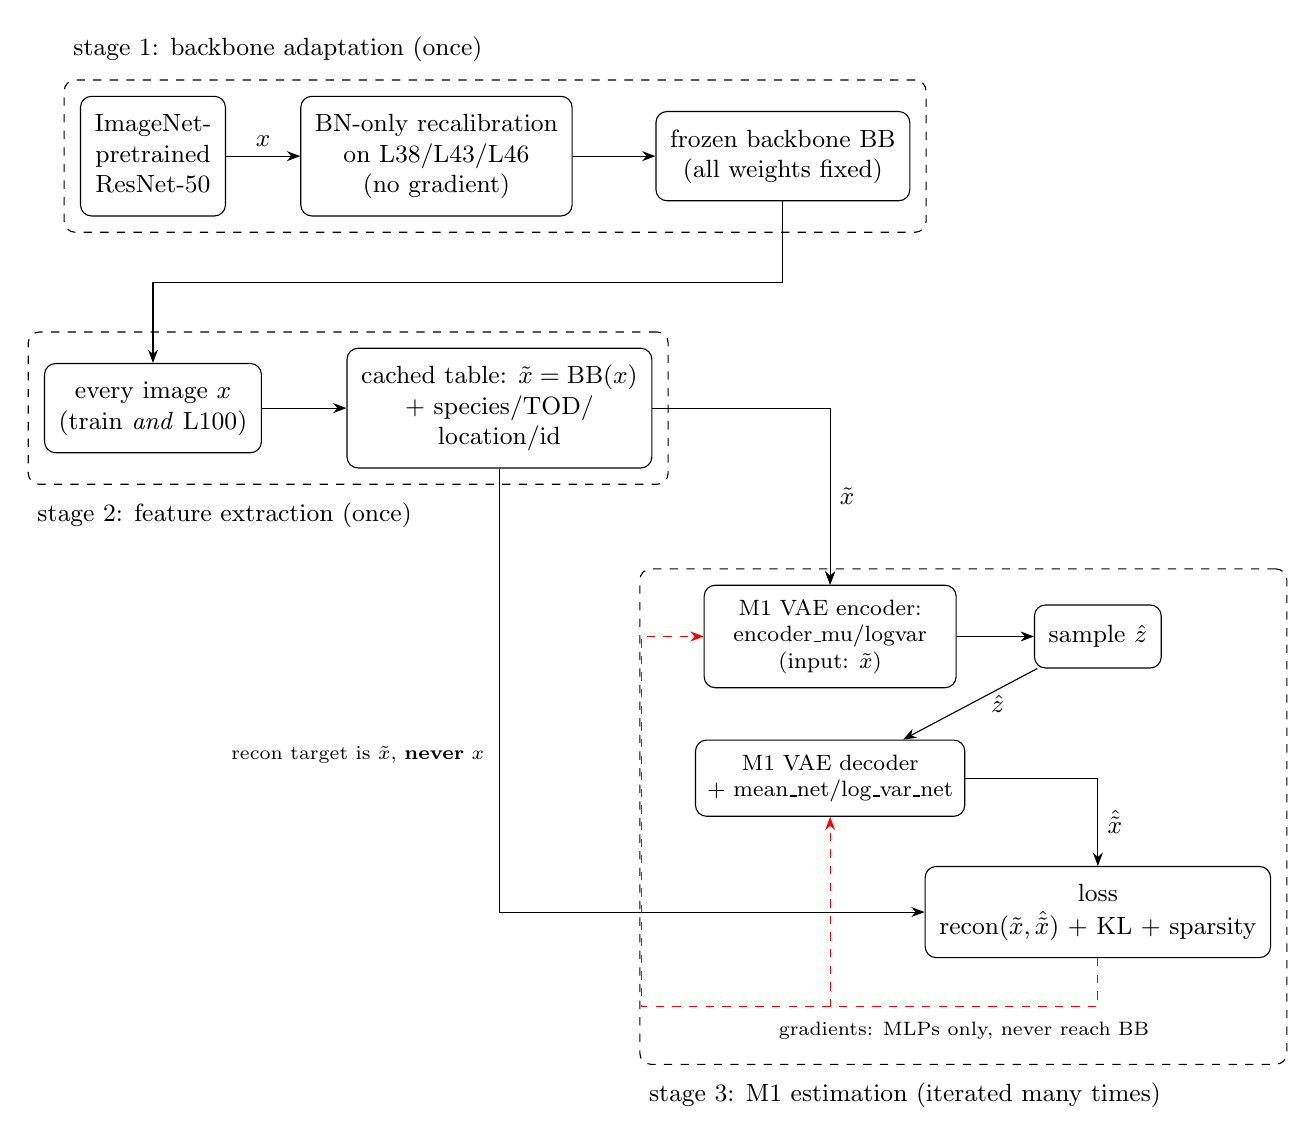
\begin{tikzpicture}[
  >=Stealth,
  font=\small,
  procnode/.style={draw,rounded corners,align=center,inner sep=1.8mm,minimum height=8mm},
  smallnode/.style={draw,rounded corners,align=center,inner sep=1.5mm,font=\footnotesize,minimum height=7mm},
  stagebox/.style={draw,dashed,rounded corners,inner sep=4mm}
]

% ---- stage 1: backbone adaptation ----
\node[procnode] (imnet) at (0,3.2) {%
  \begin{tabular}{@{}c@{}} ImageNet-\\pretrained \\ ResNet-50 \end{tabular}};
\node[procnode] (bnrecal) at (3.6,0 |- imnet.east) {%
  \begin{tabular}{@{}c@{}} BN-only recalibration \\ on L38/L43/L46 \\ (no gradient) \end{tabular}};
\node[procnode] (frozen) at (8.0,0 |- bnrecal.east) {%
  \begin{tabular}{@{}c@{}} frozen backbone $\mathrm{BB}$ \\ (all weights fixed) \end{tabular}};

\draw[->] (imnet) -- node[above] {$x$} (bnrecal);
\draw[->] (bnrecal) -- (frozen);

\begin{scope}[on background layer]
  \node[stagebox,fit=(imnet)(bnrecal)(frozen),inner sep=2mm] (stage1) {};
\end{scope}
\node[font=\small,above=1mm of stage1.north west,anchor=south west] {stage 1: backbone adaptation (once)};

% ---- stage 2: feature extraction (once) ----
\node[procnode] (allimg) at (0,0) {%
  \begin{tabular}{@{}c@{}} every image $x$ \\ (train \emph{and} L100) \end{tabular}};
\node[procnode] (cache) at (4.4,0 |- allimg.east) {%
  \begin{tabular}{@{}c@{}} cached table: $\tilde x=\mathrm{BB}(x)$ \\ + species/TOD/\\location/id \end{tabular}};

\draw[->] (frozen) -- ++(0,-1.6) -| (allimg.north);
\draw[->] (allimg) -- (cache);

\begin{scope}[on background layer]
  \node[stagebox,fit=(allimg)(cache),inner sep=2mm] (stage2) {};
\end{scope}
\node[font=\small,below=1mm of stage2.south west,anchor=north west] {stage 2: feature extraction (once)};

% ---- stage 3: M1 estimation (iterated many times) ----
\node[smallnode,minimum width=3.2cm] (m1enc) at (8.6,-2.9) {%
  \begin{tabular}{@{}c@{}} M1 VAE encoder: \\ encoder\_mu/logvar \\ (input: $\tilde x$) \end{tabular}};
\node[procnode] (zhat) at (12.0,0 |- m1enc.east) {sample $\hat z$};
\node[smallnode,minimum width=3.2cm] (m1dec) at (m1enc.south |- 0,-4.7) {%
  \begin{tabular}{@{}c@{}} M1 VAE decoder \\ + mean\_net/log\_var\_net \end{tabular}};
%\node[procnode] (xtilhat) at (zhat.south |- m1dec.east) {$\hat{\tilde x}$};
\node[procnode] (loss2) at (zhat.south |- 0,-6.4) {%
  \begin{tabular}{@{}c@{}} loss \\ recon$(\tilde x,\hat{\tilde x})$ + KL + sparsity \end{tabular}};

\coordinate (dropXt1) at (cache.east -| m1enc.north);
\draw[->]
  (cache.east) -- (dropXt1)
  -- node[right,pos=.5] {$\tilde x$}
  (m1enc.north);
\draw[->] (cache.east) -| (m1enc.north);
\draw[->] (m1enc) -- (zhat);
\draw[->] (zhat) -- node[right=4pt,pos=.5] {$\hat z$} (m1dec);
%\draw[->] (m1dec) -- (xtilhat);
%\draw[->] (xtilhat) -- (loss2);

\coordinate (dropXht1) at (zhat.south |- m1dec.east);
\draw[->] (m1dec.east) -- (dropXht1) -- node[right,pos=.5] {$\hat{\tilde{x}}$} (loss2);

\coordinate (dropT1) at (cache.south |- loss2.west);
\draw[->] (cache.south) -- (dropT1) -- (loss2.west);
\node[font=\scriptsize,align=center] at (2.6,-4.4)
  {recon target is $\tilde x$, \textbf{never} $x$};

\coordinate (dropB1) at (loss2.south |- 0,-7.6);
\coordinate (dropB2) at (m1dec.south |- dropB1.west);
\coordinate (dropB3) at (6.2,0 |- dropB1.west);
\draw[->,dashed,red] (loss2.south) -- (dropB1) -- (dropB2) -- (m1dec.south);
\draw[->,dashed,red] (dropB2) -- (dropB3) |- (m1enc.west);
\node[font=\scriptsize,align=center] (fbBlabel) at (10.3,-7.9)
  {gradients: MLPs only, never reach $\mathrm{BB}$};

\begin{scope}[on background layer]
  \node[
    stagebox,
    fit={
      (m1enc)(m1dec)(zhat)(loss2)(fbBlabel)
      ([xshift=-5mm]m1enc.west)
      ([xshift=-5mm]m1dec.west)
    },
    inner sep=2mm
  ] (stage3) {};
\end{scope}
\node[font=\small,below=1mm of stage3.south west,anchor=north west] {stage 3: M1 estimation (iterated many times)};

\end{tikzpicture}
\caption{\textbf{\nameref{sec:archB}} Stage 1 happens once and touches only BN statistics. Stage 2's
extraction pass also happens once and produces the cached table of $\tilde x=\mathrm{BB}(x)$. Stage 3
never sees $x$: its encoder takes $\tilde x$, its decoder reconstructs $\hat{\tilde x}$, and the
reconstruction term of the loss compares $\tilde x$ against $\hat{\tilde x}$, not $x$ against
$\hat x$ -- unlike \cref{fig:optA}. Gradients (dashed red) reach only the stage-3 MLPs and never the
backbone.}
\label{fig:optB}
\end{figure}

\paragraph{Why BN-only, not full fine-tuning.}
BN statistics (per-channel mean and variance) encode low-level image statistics -- illumination,
color balance, sensor response -- that differ between ImageNet and camera-trap imagery.
Recalibrating them closes much of that gap cheaply, without touching the learned convolutional
filters or anything built on top of them, needs no labels, and needs only one forward pass. It also
cannot overfit to three locations the way updating the convolutional weights (or the whole network)
could. This last point matters specifically for M1: a supervised fine-tuning objective (species
cross-entropy) has no reason to preserve location-relevant information and is, if anything, pushed to
discard it -- which would remove exactly the signal the style block $Z_s$ needs. BN-only adaptation
changes global per-channel statistics, not which features are computed, so it is far less likely to
erase that signal.

\paragraph{What reconstructing $\tilde x$ instead of $x$ actually means.}
\label{sec:archB:gap}
\Cref{def:m1,thm:ng} are stated for $X=g(Z)$ with $X$ the true observation and $g$ a $\mathrm{C}^2$
diffeomorphism onto its image (\cref{sec:ng}). Stage 3, as just described, does not fit that model. It
fits a model of $\tilde X=\mathrm{BB}(g^(Z))$ -- the composite of the true mixing $g$ with the 
backbone $\mathrm{BB}$ -- and \cite{ng2025} says nothing about this composite: $\mathrm{BB}$ is not part 
of the generative process \cref{def:m1} describes, and nothing constrains $\mathrm{BB}\circ g$ 
to be injective, differentiable in the required sense, or otherwise well-behaved, even when $g$ itself 
is.
Quite the opposite is likely: $\mathrm{BB}$ is trained (\cref{sec:pretrain}) on an objective with no
term rewarding invertibility, and both pretraining families discussed there are pushed, to different
degrees, toward \emph{discarding} exactly the nuisance/style variation that would need to survive for
$\mathrm{BB}\circ g$ to remain injective in the directions $Z_s$ occupies. \Cref{app:probe} tests
whether species and location remain \emph{linearly readable} in $\tilde x$ -- a much weaker property
than the injectivity the theorem needs, and one that can hold even when $\mathrm{BB}\circ g$ 
collapses many distinct $(Z_c,Z_s)$ onto embeddings a linear classifier can still separate but a decoder 
cannot invert.

One more point worth being explicit about, since it is easy to read the reference code the wrong way:
\cite{ng2025}'s own paper states the reconstruction loss results from the assumed 
decoder likelihood $p^{(u)}(X \mid \hat Z)$ (Gaussian, pre-specified variance), which 
doesn't hurt the identifiability argument but merely limits the scope. \nameref{sec:archB} breaks this: 
it takes that somewhat limited scope and turns it into an non-principled substitution ($\tilde x$ for 
$x$). 
\nameref{sec:archB} should therefore be read as exactly what it is: a speed-motivated heuristic that may 
or may not preserve enough of $Z$'s structure in $\tilde x$ for stage 3 to recover something useful, not 
a second, equally valid way of instantiating \cref{def:m1,thm:ng}. Whether it works is an empirical 
question this note does not resolve; \nameref{sec:archA} remains the only construction its own 
theoretical machinery actually describes.

\subsection{Pros and cons}

\paragraph{\nameref{sec:archA}}
\emph{Pros:} this is the only construction that actually instantiates $X=g(Z)$ as \cref{def:m1,thm:ng}
state it; the backbone can adapt jointly with the head, in principle giving the encoder more freedom to
place exactly the information the content/style split wants at the bottleneck; one unified model, no
separate caching step, no intermediate object standing in for $x$.
\emph{Cons:} every iteration runs a full ResNet-50 forward and backward pass on raw images -- hours,
not minutes, in your own experience -- while the M1 estimator itself is still being iterated (the
five open items closing \cref{app:code}: $u$-dependent offset/mean, per-coordinate mechanisms, the
sink-freezing test, the optimizer overlap, the dead code), so every one of those iterations would
carry the full backbone cost; the loss (\mbox{reconstruction + KL + sparsity}) has no term that 
specifically rewards keeping location information, so end-to-end gradient pressure can push the backbone 
to discard exactly the style-relevant cues $Z_s$ is supposed to capture; two learning problems with
different dynamics -- representation learning and causal/structural discovery (Adam on most
parameters, a separate SGD gate optimizer on the adjacency matrix, \cref{app:code}) -- are coupled
through shared backbone gradients, harder to diagnose than training the small MLPs alone; only three
training locations, so fine-tuning the whole backbone risks overfitting its features to those three
sites rather than to the location-invariant/location-varying split M1 assumes; and even here, nothing
guarantees the backbone itself is injective (any convolutional network with pooling generically is
not) -- end-to-end training only supplies gradient \emph{pressure} toward retaining what reconstruction
needs, not a proof that it does.

\paragraph{\nameref{sec:archB}}
\emph{Pros:} iteration is minutes rather than hours, which matters given how much of the M1 estimator
is still design rather than implementation. Extraction is a single pass per image, cached once;
everything downstream is plain backprop on $\sim\!3000$-dim vectors, cheap to re-run many times over.
\Cref{app:probe}'s linear-probe diagnostics give a cheap, checkable precondition test -- whether
species/location information survives at all in $\tilde x$ -- before committing to this heuristic for a
given backbone; passing that check narrows candidates but, as \cref{sec:archB:gap} explains, does not
establish that stage 3's fitted model bears any proven relationship to the true $(Z_c,Z_s,\Gc)$.
\emph{Cons:} \cref{sec:archB:gap} is the central one and subsumes the more specific concerns below --
this option does not implement \cref{def:m1,thm:ng} at all, and no identifiability result in this note
applies to it. More specifically: a hard ceiling set by the backbone -- whatever style/location
information is not present in $\tilde x$, even after BN-only recalibration, cannot be recovered by any
downstream causal method; $\tilde x$ is not shaped by the M1 reconstruction objective itself, so subtle
style cues a jointly-trained encoder might have preserved for reconstruction's sake could be missing;
changing the layer(s), pooling, or backbone means re-extracting and re-caching the whole table (cheap,
but a step that end-to-end training does not need).

\subsection{Recommendation}
\label{sec:rec}
Use \nameref{sec:archB} first, but as a heuristic, not as a theory-matching choice:
\cref{sec:archB:gap} means nothing in this note guarantees it recovers anything. The reasons to start
there are practical only. First, iteration speed: \cref{app:code} closes with five concrete open
changes to the reference implementation, each of which still needs to be tried and likely revised,
which is only practical at minutes per run rather than hours. Second, it decouples backbone selection
(checkable once, cheaply, via \cref{app:probe}) from estimator design (iterated many times), so a bad
backbone choice does not have to be discovered by watching the M1 estimator itself fail to converge.
Third, \nameref{sec:archA} does not automatically avoid the injectivity problem either -- any
convolutional backbone with pooling is generically non-injective regardless of how it is trained -- so
paying its much higher cost does not, by itself, buy a proof that the resulting model matches
\cref{def:m1}; it only removes the specific, additional substitution of $\tilde x$ for $x$ that
\cref{sec:archB:gap} describes, restoring $x$ as the reconstruction target the theorem is actually
about.

Given this, treat \nameref{sec:archB} as an exploratory, cheap-to-iterate first pass -- useful for
developing and debugging the prior/graph design of \cref{sec:use} -- and \nameref{sec:archA} as the one
construction whose relationship to \cref{def:m1,thm:ng} this note can actually state precisely: to be
used once the design stabilizes enough to justify its cost, and to check whether conclusions reached
under \nameref{sec:archB} survive when $x$, rather than $\tilde x$, is reconstructed.

\subsection{Pretraining objective for the backbone: supervised vs.\ self-supervised}
\label{sec:pretrain}
What matters for M1 is not raw discriminative accuracy on ImageNet classes but whether the embedding
still contains \emph{both} kinds of signal the split needs to separate afterward: content (species,
time of day) and style (location/camera cues). This choice matters most for \nameref{sec:archB}, where
whatever the backbone discards is discarded permanently -- stage 3 never touches $\mathrm{BB}$ again.
Under \nameref{sec:archA} the same choice still matters as the initialization the end-to-end
fine-tuning starts from, though there gradient pressure from the M1 loss can, in principle but without
guarantee, partially recover discarded signal. If either kind of signal is missing after pretraining
(and, for \nameref{sec:archB}, after BN-only recalibration), no downstream causal machinery in
\cref{app:code} can recover it -- this is exactly the feature-extraction ceiling noted as a con of
\nameref{sec:archB} above (\cref{sec:archB:gap}).

\paragraph{Supervised ImageNet pretraining.}
The objective is cross-entropy on object categories that do not correlate with camera exposure,
background statistics, or viewpoint, so nothing in the loss rewards keeping that information;
supervised features are, generically, pushed toward invariance to exactly this kind of within-class
nuisance variation. For M1 this is close to the worst case among the candidates: the pretraining
objective actively works against keeping the style signal the style block needs.

\paragraph{Self-supervised: SimCLR, MoCo v2, MoCo v3, SimSiam.}
All four train invariance to a shared, standard augmentation recipe -- random-resized crop, color
jitter, occasional grayscale, Gaussian blur, horizontal flip -- rather than invariance to a fixed
label set. What differs between them is the loss and the negative-pair mechanics (InfoNCE with a
large batch for SimCLR; a momentum encoder plus a memory queue for MoCo v2; a momentum encoder plus a
predictor without a memory queue for MoCo v3; a predictor with stop-gradient and no negatives at all
for SimSiam), which mainly affects training stability and representation quality for the downstream
discriminative task, not \emph{which} low-level factors get suppressed. So there is no a priori
reason to expect any one of the four to retain systematically more or less location/style information
than the others. Two caveats, both empirical rather than settled by the choice of method: (a) color
jitter and blur do push toward suppressing some of the brightness/exposure cues that matter for
time-of-day/style in TI, less aggressively than a labeled cross-entropy objective but not zero; (b)
none of the four ever see location or time-of-day labels during pretraining, so whatever style signal
survives is incidental to the augmentation recipe, not something the objective was built to preserve.

\paragraph{Recommendation.}
Prefer self-supervised pretraining over supervised, generically, since supervised is the one option
whose objective actively works against what M1 needs. Among SimCLR, MoCo v2, MoCo v3 and SimSiam
there is no first-principles reason to prefer one for style preservation; choose empirically, using
the linear-probe step of \cref{app:probe} (species accuracy plus within-species location accuracy on
cached features) over whichever of the four you already have trained, and keep the supervised
ResNet-50 only as a baseline/comparison point rather than a primary candidate.

\subsection{Verification of Recommendations}
\label{sec:verify}
Before investing in \nameref{sec:archB} for a given backbone, run the test outlined in \cref{app:probe}
to compare candidates. Per \cref{sec:archB:gap}, a pass there rules out only the worst case -- a
backbone that has discarded species or location information outright -- it does not establish that the
backbone, or its composition $\mathrm{BB}\circ g$ with the true mixing, is close to the injective map \cref{thm:ng} requires, and no diagnostic in this note checks that directly. \Cref{sec:archA} needs no equivalent gate, since it does not introduce $\tilde x$ or $\mathrm{BB}$ as a separate, unexamined step in the first place.


% =====================================================================
\section{Pseudo-injective estimation: replacing the flow head with a regularized VAE}
\label{sec:pseudoinj}

\Cref{sec:flow} proposed a flow head to get an exactly invertible $g$.
It was abandoned before implementation: an exactly invertible map cannot reduce dimension
(\cref{sec:flow:motivation}), so a square injective flow head is structurally the wrong shape for M1, 
which needs roughly ten output latents, not a $150{,}528$-dimensional one. This section proposes what 
replaces it: not an exact diffeomorphism, but a pair of networks -- a frozen, pretrained backbone and a 
trainable head -- each carrying an explicit, measurable regularizer that keeps them \emph{close to} 
\textbf{injective}, while actually reducing dimension the way \nameref{sec:archB} does. 
We first restate the problem this is meant to solve, then the alternatives that were considered and set 
aside, then the two pieces of the proposed pipeline (\cref{sec:pseudoinj:invae,sec:pseudoinj:blae}), 
then a first, wrong version of the
training objective and why it had to be corrected (\cref{sec:pseudoinj:jacobian}), then the corrected
architecture (\cref{sec:pseudoinj:arch}), and finally an explicit list of gotchas
(\cref{sec:pseudoinj:gotchas}) that a reader implementing this should not discover the hard way.

\subsection{The problem this section answers}
\label{sec:pseudoinj:problem}
\Cref{sec:archB:gap} already states the gap in \nameref{sec:archB} plainly: a frozen ResNet-50 is
provably non-injective (any pooling convnet is), so nothing constrains $\mathrm{BB}\circ g^{-1}$ to be
injective, differentiable, or otherwise well-behaved, and the gap is \emph{unexamined} -- nothing in the
pipeline measures how bad it is. \Cref{sec:flow} closed that gap exactly, at the cost of being unable to
reduce dimension. What is wanted is a middle position: a backbone and a head that are not exactly
injective, but whose deviation from injective is bounded and estimated, not ignored, while still landing
at M1's small latent dimension (\emph{``pseudo-injective''}).

\subsection{Alternatives considered and set aside}
\label{sec:pseudoinj:discarded}
\begin{itemize}[leftmargin=1.5em]
\item \textbf{Rectangular (injective) flows} \cite{caterini2021}. These are the flow family that can, in
      principle, reduce dimension while staying exactly injective, by computing the Gram determinant
      $\det(J^\top J)^{1/2}$ instead of a square Jacobian determinant (\cref{sec:flow:injective}). Set
      aside: the published results barely reach CIFAR-10 scale, not ImageNet-scale full-resolution 
      images, and computing (or differentiating) the Gram determinant is itself an open research 
      problem, not an engineering cost.
\item \textbf{A $(z,w)$ padding variant.} Keep an exactly bijective, dimension-preserving flow as in
      \cref{sec:flow}, but declare only the first $\sim\!10$ coordinates of its output ``$z$'' (M1's
      latent) and treat the rest as a nuisance padding vector $w$, discarded after training. Set aside:
      this sits outside \cref{thm:ng} as written (the theorem is stated for $Z$ itself, not a marginal or
      a projection of a larger vector with no constraint tying $w$ to anything), and it does not obviously
      buy anything \nameref{sec:archB} does not already give more cheaply.
\end{itemize}

\subsection{IN-VAE: a pretrained, frozen, reconstruction-trained backbone}
\label{sec:pseudoinj:invae}
\textbf{What it is.} A large, pretrained image autoencoder of the kind used as the first stage of latent
diffusion pipelines: an encoder/decoder pair trained end-to-end on a reconstruction (plus, depending on
the variant, adversarial and/or perceptual) objective at ImageNet scale, whose \emph{encoder} we reuse
frozen as BB, exactly as \nameref{sec:archB} reuses a frozen ResNet-50. We call this class \textbf{IN-VAE}
in this note: pseudo-injective not because any Jacobian argument certifies it, but because reconstruction
training directly rewards the encoder-decoder pair for approximately undoing each other, which a
classification objective (plain ResNet-50, or the supervised-pretraining case of \cref{sec:pretrain}) has
no reason to do at all. Unlike \nameref{sec:archB}'s pooled $\sim\!3072$-dim vector, IN-VAE's output is a
\emph{spatial} latent, a tensor of shape $C\times h\times w$ (concretely $32\times16\times16$ for the
chosen candidate, \cref{sec:pseudoinj:arch}), not a flattened, globally pooled embedding -- this is
relevant to the head architecture below.

\textbf{Candidates surveyed.} SD-VAE kl-f8 (embedding width $4096$),
\footnote{the regularization type on the latent: KL-regularized, $\times$8 spatially downsampled}
the IN-VAE/REPA-E baseline used in
this note ($8192$), E2E-VAE ($8192$-class, but its representation-alignment loss is trained to match a
downstream generative model's preferred feature geometry, which is exactly the kind of pressure
\cref{sec:pretrain} already flags as likely to squeeze out style/location cues), FLUX/SD3 VAE
($16384$), DC-AE, and MAETok/STELLAR (semantically-shaped tokenizers, same style-squeezing risk as
E2E-VAE, for a different reason: their objective explicitly rewards semantic/content compression). Every
candidate carrying this alignment or semantic-shaping risk -- E2E-VAE, MAETok, STELLAR -- must be screened
with the linear-probe diagnostic of \cref{app:probe} (species accuracy plus within-species location
accuracy) before it is used, exactly as \cref{sec:pretrain} already requires for the ResNet-50 case; none
of them is used or discussed further in this note.

\textbf{Why IN-VAE (the REPA-E-style baseline) \cite{leng2025repae} is the default here.} It is trained on plain reconstruction
(plus generic perceptual/adversarial terms), with no alignment or semantic-shaping loss pulling it toward
discarding style/location information; its embedding width ($8192$, i.e.\ $32\times16\times16$) is
comparable to the other non-flagged candidates; and, as an encoder-decoder pair with a released,
well-tested implementation (Hugging Face \texttt{diffusers.AutoencoderKL} \cite{aekl}), it needs no 
bespoke pipeline code, only a frozen forward pass -- the same iteration-speed argument \cref{sec:archB} 
already makes for a frozen backbone. Everything from here on assumes this choice; it should still pass 
\cref{app:probe}'s screen before being trusted, the same as any candidate.

\subsection{BLAE: an injective/bi-Lipschitz regularizer for the trainable head}
\label{sec:pseudoinj:blae}
\textbf{What it is.} Zhan et al.\ \cite{zhan2026blae} assume that high-dimensional data resides
on a $k$-low-dimensional manifold $\Mk \subset \R^m,\ k = \dim(\Mk)$ and that there's an autoencoder 
that learns this intrinsic representation through a pair of parametrized mappings 
$(\E_\theta,\D_\phi)$:
\begin{itemize}
\item The encoder $\E_\theta : \R^m \to \R^n (k < n \ll m)$ compresses data onto a low-dimensional 
      latent space;
\item The decoder $\D_\phi : \R^n \to \R^m$ reconstructs the original data from the latent 
representation.
\end{itemize}

They propose two losses to add to an otherwise ordinary autoencoder, meant to push its encoder 
toward being injective without requiring an exactly invertible architecture:
\begin{itemize}[leftmargin=1.5em]
\item an \emph{injective} (separation) loss, which penalizes distinct inputs landing too close 
      together in latent space (their Theorem~1 gives a separation criterion);
\item a \emph{bi-Lipschitz} relaxation term, which additionally penalizes local distortion of
      \emph{geodesic} distances between the ambient data (estimated once via an Isomap-style 
      shortest-path computation) and Euclidean distances between the corresponding latents; the 
      paper argues (their Theorems~3-4) this relaxation is admissible at $O(n)$ latent dimensions, 
      where a hard embedding guarantee would need $O(k^2)$.
\footnote{According to the Nash embedding theorem \cite{nash1956}, a $k$-dimensional compact 
Riemannian manifold requires a latent dimension of $O(k^2)$ to guarantee an isometric embedding
(distance preserving); the required latent dimension $n$ satisfies 
$\frac{k(k+1)}{2} \le n \le \frac{k(3k+11)}{2}$.}
\end{itemize}
This is a \emph{trained regularizer}, not a proof of injectivity, and it is unproven at ImageNet 
scale: the paper's own experiments are Swiss Roll, dSprites, MNIST, CIFAR-10, Bird, and Teapot.

\textbf{What is reusable from the released repository, and what is not.} The repository's dataset-
specific autoencoder classes are toy-sized and toyishly-implemented (latent dims $2$--$16$, small 
fixed image sizes) and not directly usable.
What \emph{is} architecture-agnostic and directly reusable: the injective loss and the bi-Lipschitz 
term themselves (they take only a latent batch and a precomputed geodesic-distance table, nothing
dataset-specific), and the geodesic-distance-table computation (\cref{sec:pseudoinj:gotchas} 
discusses its cost at TI scale). \textbf{No VAE variant is released}: a stochastic BL-VAE is 
described only in the paper's Appendix~C.6.2, demoed on Swiss Roll, and never shipped in the code 
(a repository search for VAE/reparameterization/log-variance/KL code returns nothing in Python 
files; there's a Jupyter notebook with some VAE-denoted variables, but their examination shows that 
this is not a true VAE).

\subsection{Why a VAE head, and not a deterministic autoencoder}
\label{sec:pseudoinj:jacobian}
\textbf{The question.} The exact change-of-variables objective of \cref{eq:flow-nll} needs a volume
term. Neither IN-VAE's encoder nor a BLAE-regularized head is a square, exactly invertible map, so the
term is the Gram determinant $\det(J^\top J)^{1/2}$ of \cref{sec:flow:injective}, not an ordinary
determinant. The question is whether this objective can be used for the head. An earlier version of this
note said that $J$ ``cannot be computed''. That statement is too strong, and the justification below
replaces it.

\textbf{What is and is not the obstacle.}
\begin{itemize}[leftmargin=1.5em]
\item \emph{Computing $J$ is not the obstacle.} The trainable decoder maps a latent of dimension $10$ to
      the image-side tensor, so its Jacobian has only $10$ columns and $J^\top J$ is a $10\times10$
      matrix. Forward-mode differentiation gives $J$ with about $10$ passes per sample. This is exactly
      what the bi-Lipschitz term of \cref{sec:pseudoinj:blae} already does when it evaluates the decoder
      Jacobian. That term is a regularizer, however, and only needs approximate singular values. A
      likelihood needs the exact $\log\det$ and its gradient at every step.
\item \emph{Cost is a real but secondary obstacle.} Backpropagating through $\log\det(J^\top J)$ means
      differentiating through forward-mode Jacobians of a convolutional decoder with attention, at every
      training step and for every sample. The attention blocks must also be run with the unfused (math)
      backend, because the fused kernels have no forward-mode rule. This is affordable for a
      regularizer weighted by a small coefficient, but it is a heavy price for the main objective.
\item \emph{The Gram determinant does not factorize over stages.} For square maps, $\log|\det|$ of a
      composition is the sum of the per-stage terms, which is what made the flow section tractable
      (\cref{eq:flow-jac-split}). For non-square maps it is not. The volume term of the composite
      ``frozen IN-VAE decoder after head decoder'' is not the sum of a backbone term and a head term, so
      the frozen backbone cannot be handled separately.
\item \emph{The main obstacle: the density is degenerate.} A deterministic decoder from a
      $10$-dimensional latent has an image that is a $10$-dimensional manifold inside a much
      larger space. The pushforward of $p_{\hat Z}$ is then supported on that manifold and has no density
      with respect to Lebesgue measure on the large space. The change-of-variables formula yields a
      density only with respect to the surface measure of the manifold, and it is meaningful only for
      points that lie on it. Real images (or their cached embeddings) never lie exactly on it, so
      $\log p_X(x)$ is undefined without an additional off-manifold noise model. This holds no matter how
      cheaply the Gram determinant could be computed.
\end{itemize}

\textbf{The rejected first candidate.} 
The first idea was to keep BLAE's deterministic autoencoder
and evaluate M1's prior at the single encoded point $\hat z=\mathrm{Enc}(x)$, as in
\cref{eq:flow-prior-term}, with no volume term. This silently replaces the target $\log p_X(x)$ by
$\log p_{\hat Z}(\hat z\mid u)$, which is a poor proxy to the extent that the encoder is non-injective.
Nothing in that loss bounds or even reports the gap.

\textbf{Decision: use a VAE for the trainable head.} A VAE needs neither the Gram determinant nor the
manifold assumption. The Gaussian decoder with fixed variance is exactly the off-manifold noise model
that makes the density on the large space well defined, and the ELBO then requires no Jacobian at all.
This is why Ng et al.'s estimator (\cref{app:code}) and \nameref{sec:archA}/\nameref{sec:archB} all use
an ELBO. The price is the usual, already accepted approximation: $q(\hat Z\mid X)$ only approximates the
true posterior, and the reconstruction term only penalizes the cases where decoding fails to invert
encoding. The Jacobian then appears in exactly one place, the BLAE bi-Lipschitz regularizer, where an
approximate, weighted use is sufficient.

\subsection{The resulting architecture}
\label{sec:pseudoinj:arch}
\begin{enumerate}[label=(\arabic*),leftmargin=2em]
\item \textbf{Frozen backbone.} IN-VAE's pretrained encoder (\cref{sec:pseudoinj:invae}), run once 
       per image, cached, exactly as \nameref{sec:archB} caches $\tilde x=\mathrm{BB}(x)$ -- except 
       here $\tilde x$ is the spatial IN-VAE latent, a $32\times16\times16$ tensor, not a pooled 
       ResNet vector.
%-----------------
\item \textbf{Trainable head.} A \emph{fresh, untrained} instance of Hugging Face's
      \texttt{diffusers.AutoencoderKL} \cite{aekl} (not a pretrained checkpoint), 
      used \emph{unmodified} -- rather 
      than editing its \texttt{quant\_conv} and \texttt{post\_quant\_conv} internals, two small 
      trainable wrapper blocks sit outside it and convert between its native spatial latent and M1's 
      flat vector.

      \textbf{Sizing the stock module.} \texttt{AutoencoderKL} \cite{aekl} is configured, but not 
      altered internally, to fit the $32\times16\times16$ IN-VAE input:
      \begin{itemize}[leftmargin=1.3em]
      \item In diffusers the last encoder stage does not downsample, so \texttt{N} stages give 
            \texttt{N-1} halvings.
            
            \texttt{down\_block\_types = ("DownEncoderBlock2D", "DownEncoderBlock2D",}\\ 
            \texttt{"DownEncoderBlock2D")} (3 stages,
            $16\to8\to4$), with the symmetric \texttt{up\_block\_types} triple;
      \item \texttt{block\_out\_channels = (32, 64, 128)};
      \item \texttt{layers\_per\_block = 1};
      \item \texttt{in\_channels = out\_channels = 32};
      \item \texttt{latent\_channels} left at whatever stock value keeps \texttt{quant\_conv}/
            \texttt{post\_quant\_conv} well-defined (e.g.\ $4$); this is \emph{not} M1's $\sim\!10$-
            dim latent -- that reduction happens entirely in the wrapper blocks below, outside the 
            module.
      \end{itemize}
      With this config, stock \texttt{AutoencoderKL.encode} returns its own spatial latent 
      distribution at $4\times4\times4$ (i.e.\ \texttt{latent\_channels}$=4$, spatial size 
      $4\times4$), unchanged from the library's normal behavior.

      \textbf{Pre-block (after \texttt{AutoencoderKL.encode}, before M1).} Flatten (or global-average-
      pool) the module's own $4\times4\times4$ output, then a single linear layer maps this flat vector 
      to M1's $20$ scalars $(\hat\mu,\hat{\log\sigma^2})$ (i.e.\ $10$ content/style latents). This 
      linear layer is the actual dimensionality-reducing step; \texttt{AutoencoderKL} itself is never 
      told about, and never computes, the $10$-dim target.

      \textbf{Post-block (after M1's prior/loss, before \texttt{AutoencoderKL.decode}).} A single linear
      layer expands the sampled $10$-dim $\hat z$ back to a flat $4\times4\times4$ vector, reshaped to
      $4\times4\times4$ and passed into stock \texttt{AutoencoderKL.decode} unmodified.

      \textbf{Why this is preferred over editing the module.} The pre/post linear layers are the only
      hand-written, unvalidated pieces; \texttt{AutoencoderKL}'s own encode/decode path, KL
      reparameterization, and internal conv blocks stay exactly as tested and released, with no risk of 
      a silent behavioral change from touching \texttt{quant\_conv}/\texttt{post\_quant\_conv} directly. 
      The cost is one extra pair of thin layers and one more bottleneck seam (module output $\to$ M1 
      vector) to account for when tracing where distortion enters the pipeline 
      (\cref{sec:pseudoinj:gotchas}).
%-----------------
\item \textbf{M1 prior, unchanged.} The content/style ANM prior of \cref{sec:use} -- \texttt{mean\_net},
      \texttt{log\_var\_net}, the adjacency \texttt{adj\_mat}, sink-freezing -- sits on top of the head's
      output exactly as in \cref{app:code}; nothing about the prior side changes here, only the recognition
      network $q(\hat Z\mid X)$ feeding it.
\item \textbf{BLAE losses, added to the head's training, computed on $\hat\mu$.} The injective (separation)
      loss and the bi-Lipschitz term of \cref{sec:pseudoinj:blae} are added to the head's loss, evaluated
      on the posterior mean $\hat\mu$ (never on a noisy sample $\hat z=\hat\mu+\epsilon$, since the
      geodesic-preservation objective is inherently a statement about a deterministic map -- the
      reparameterization noise must not enter this term). The geodesic-distance table (\texttt{GeoD}) is
      built once from the cached IN-VAE embeddings of the training-location images.
\end{enumerate}
The resulting per-image loss, replacing \texttt{Trainer.step} of \cref{app:code} on the head side:
\begin{equation}
\begin{aligned}
\mathcal L(x,u) &= \lambda_{\mathrm{kl}}\,\mathrm{KL}\bigl(q(\hat Z\mid x)\,\|\,p_{\hat Z}(\hat Z\mid u)\bigr) \\
&+ \lambda_{\mathrm{rec}}\,\mathrm{recon}(\tilde x,\hat{\tilde x}) \\
&+ \lambda_{\mathrm{inj}}\,\ell_{\mathrm{inj}}(\hat\mu) \\
&+ \lambda_{\mathrm{biLip}}\,\ell_{\mathrm{biLip}}(\hat\mu,\mathtt{GeoD}) \\
&+ \lambda_{\mathrm{sparse}}\,\ell_{\mathrm{sparse}}(\hat A) \\
&+ \lambda_{\mathrm{moral}}\,\ell_{\mathrm{moral}}(\hat A, A^{t-1}),\footnotemark\\
&\quad A^{t-1}\ \text{is the binary adjacency matrix estimated in the previous} \\
&\quad \text{(i.e.,}\ (t\!-\!1)\text{-th) iteration}.
\end{aligned}
\label{eq:pseudoinj-loss}
\end{equation}
\footnotetext{Ng implementation dropped the moral loss term in their implementation --
see \cref{app:code:lossterms}.}%
where $\tilde x$ is the cached IN-VAE embedding (the reconstruction target, one level removed from the raw
image, as in \nameref{sec:archB}), and the first, second and fifth terms are exactly \cref{app:code}'s
\texttt{loss\_kl}, \texttt{loss\_rec} and \texttt{loss\_sparsity}. \emph{No Jacobian term appears anywhere
in \cref{eq:pseudoinj-loss}}, by the decision of \cref{sec:pseudoinj:jacobian}.

\subsection{Why this is more principled than plain Option B -- and what it still is not}
\label{sec:pseudoinj:principled}
Both stages of this pipeline carry an explicit, measurable regularizer toward injectivity: IN-VAE's
reconstruction training (rewards approximate invertibility directly, unlike a classification objective);
the head's injective and bi-Lipschitz losses (bound local distortion of distances, with a stated theoretical
target). Plain \nameref{sec:archB} has neither -- \cref{sec:archB:gap}'s gap is totally unexamined there.
This is genuinely better: instead of an unknown, unbounded gap, the gap here is a quantity the bi-Lipschitz
constants put a number on.

It is not a proof of injectivity, and \cref{thm:ng}'s hypothesis -- $g$ an exact $C^2$ diffeomorphism onto
its image -- is still, strictly, violated by both IN-VAE and the head, in exactly the same
\emph{category} of gap \cref{sec:archB:gap} already names for plain Option B. The honest claim is:
\textbf{bounded and diagnosable distortion, not solved injectivity.} This should be stated exactly this
plainly wherever this pipeline is invoked elsewhere in the note, the same way \cref{sec:archB:gap} states
its own gap without softening it.

\subsection{Gotchas}
\label{sec:pseudoinj:gotchas}
\begin{itemize}[leftmargin=1.5em]
\item \textbf{KL vs.\ injective/bi-Lipschitz tension, and the limits of what can be said about it.} The
      KL term in \cref{eq:pseudoinj-loss} rewards posterior compression toward the prior; the injective and
      bi-Lipschitz terms reward keeping distinct inputs' encodings apart. These pull in opposite
      directions. The most that can honestly be said at present: Zhan et al.\ state that BLAE's losses can
      be added to a VAE, and presumably tested this on a toy example, but \textbf{no such implementation
      was released} (\cref{sec:pseudoinj:blae}), so this note's combination of a fresh
      \texttt{AutoencoderKL} head with BLAE's losses is unverified engineering, not a reproduction of a
      published result. $\lambda_{\mathrm{kl}}$ against $\lambda_{\mathrm{inj}},\lambda_{\mathrm{biLip}}$
      needs to be tuned empirically, with no prior result to anchor the starting point.
\item \textbf{Extreme compression ratio.} \texttt{AutoencoderKL}'s stock configurations target hundreds 
      to thousands of latent channels, not $\sim\!10$; squeezing this far raises real underfitting/
      posterior-collapse risk. \Cref{sec:pseudoinj:arch} above hand-tunes depth and channel width down 
      for this reason, but the $4\times4\times4=64$ scalars $\to20$-scalar bottleneck introduced there 
      is itself a 
      further, unusually aggressive compression step (pooling/flattening plus one linear layer) with no 
      precedent in the stock class to calibrate against.
\item \textbf{Fresh initialization, no pretraining head start.} Unlike IN-VAE, the head is trained from
      scratch on $\sim\!18\mathrm{k}$ TI images alone.
\item \textbf{BLAE losses must be computed on $\hat\mu$, never on the sampled $\hat z$} -- this needs to 
      be explicit in the loss code, not left implicit, since it is easy to accidentally apply it after 
      the reparameterization step.
\item \textbf{No VAE implementation exists in the BLAE repository at all}; combining a tested
      \texttt{AutoencoderKL} \cite{aekl}with a from-scratch reimplementation of BLAE's loss terms is 
      novel engineering that must be built and validated, not assumed to inherit the paper's toy-scale 
      results.
\item \textbf{Spatial, not pooled, embeddings, and a non-standard bottleneck.} IN-VAE's output is a
      $32\times16\times16$ tensor, unlike \nameref{sec:archB}'s flat pooled $\sim\!3072$-dim vector; the
      head must be conv-based to consume this properly, not a bare MLP as in \texttt{app:code}'s
      \texttt{encoder\_mu}/\texttt{encoder\_logvar}. Because stock \texttt{AutoencoderKL} \cite{aekl} 
      has no
      built-in path from a spatial bottleneck to a flat per-image vector, the
      \texttt{quant\_conv}/\texttt{post\_quant\_conv} replacement in \cref{sec:pseudoinj:arch} is
      hand-written and untested code, not a configuration of an existing, validated path.
\item \textbf{Resolution mismatch.} IN-VAE candidates (including the chosen one) are pretrained at 
      $256$px; this note's pipeline currently assumes $224$px throughout (\cref{sec:archB}) and needs 
      updating if this backbone is adopted.
\item \textbf{Screened candidates.} E2E-VAE and MAETok/STELLAR carry alignment or semantic-shaping losses
      that risk discarding style/location signal, the same failure mode \cref{sec:pretrain} already flags
      for supervised ImageNet pretraining; neither is used here, and any candidate -- including the chosen
      IN-VAE -- still needs to clear \cref{app:probe}'s linear-probe screen before being trusted.
\item \textbf{The geodesic-distance table (\texttt{GeoD}) cost, now one stage removed from pixels.} Building
      \texttt{GeoD} on the cached IN-VAE embeddings ($N\!\approx\!18\mathrm{k}$, still $\sim\!8192$-dim)
      is a one-time precompute, run once per choice of backbone/embedding (not per epoch, not per
      minibatch), with two distinct costs:
      \begin{itemize}[leftmargin=1.3em]
      \item \emph{Pairwise-distance step}, $O(N^2d)$. Naive broadcasting would try to materialize an
            $N\times N\times d$ tensor ($\sim\!10$TB at $N=18\mathrm{k}$, $d=8192$) -- infeasible. Use the
            Gram-matrix identity $\|x-y\|^2=\|x\|^2+\|y\|^2-2x^\top y$ (one matmul, $O(Nd+N^2)$ peak memory)
            instead; confirm \texttt{sklearn}'s \texttt{kneighbors\_graph} is honoring its
            \texttt{working\_memory} row-chunking rather than being overridden. Further remedies if still
            too costly: reduce $d$ via PCA/random projection before this step ($8192\to256$,
            Johnson-Lindenstrauss-justified, $\sim\!32\times$ cheaper); approximate kNN (FAISS/HNSW,
            GPU-capable, never materializes a dense pairwise matrix); or a landmark-Isomap variant (exact
            geodesics from a landmark subset only, e.g.\ $2\mathrm{k}$ of $18\mathrm{k}$, nearest-landmark
            interpolation for the rest, turning $O(N^2)$ into $O(N_LN)$).
      \item \emph{All-pairs shortest-path step}, $O(N^2\log N)$ (Dijkstra/Johnson's algorithm over the
            resulting sparse $k$-NN graph). Remedies: shard per-source Dijkstra runs across CPU processes
            (embarrassingly parallel); reuse the landmark trick above to cut the number of source runs from
            $N$ to $N_L$; confirm \texttt{scipy} is selecting Johnson's algorithm (\texttt{method='J'}) for
            the sparse case rather than defaulting to a slower per-node routine.
      \end{itemize}
\item \textbf{Memory.} The dense $N\times N$ \texttt{GeoD} table ($\sim\!1.3$GB at $N=18\mathrm{k}$)
      belongs on CPU (plain array, or \texttt{numpy.memmap} if it outgrows RAM) and should never be copied
      to GPU in full; slicing a small $B\times B$ submatrix per minibatch on CPU before moving only that
      slice to GPU (the pattern already used for \texttt{GeoD} indexing) is correct and should be kept.
      The real risk is upstream, in the pairwise-distance step: doing that naively on GPU can exhaust GPU
      memory before \texttt{GeoD} is even built; the same Gram-matrix trick, or a GPU-batched approximate-
      kNN library, avoids this. If \texttt{GeoD} itself is still tight on a given host, storing it as
      \texttt{float16} (halving it to $\sim\!650$MB at $N=18\mathrm{k}$) is an acceptable fallback, since
      geodesic distances are a regularization target, not a quantity needing \texttt{float32} precision.
\item \textbf{Still not exact injectivity.} As stated in \cref{sec:pseudoinj:principled}, this pipeline
      bounds and quantifies the gap from \cref{thm:ng}'s exact-diffeomorphism hypothesis; it does not
      close it. Any downstream use of this note's identifiability results should carry this caveat forward
      explicitly.
\end{itemize}

% ---------------------------------------------------------------------
% Bibliography entries this section assumes but that are not yet in biblio.tex:
%   zhan2026blae   -- Zhan et al., "BLAE" / bi-Lipschitz autoencoder, arXiv:2604.06701
%   leng2025repae  -- Leng et al., REPA-E (or the specific IN-VAE checkpoint's source paper)
%   (optionally: a citation for SD-VAE/latent-diffusion VAEs and the original
%    VAE paper (Kingma and Welling), if you want them cited by name rather
%    than referred to descriptively as above)
% Also not yet defined in this note: \label{app:code:lossterms} referenced in the
% footnote on the moral-loss term -- point it at the right subsection of app_ng_reference_impl.tex
% (currently that file has no such label).

% =====================================================================
\section{Assumptions and limitations}
\label{sec:limits}
\begin{itemize}[leftmargin=1.5em]
\item \textbf{Gaussian additive noise for all latents.} This is what \cref{thm:ng} requires; for an
      isolated style latent the sink property is only needed trivially, but relaxing the Gaussianity
      for that block is not covered by the theorem. The choice between the ANM and the heteroscedastic
      model is discussed in \cref{app:hnm}.
\item \textbf{Regularity.} $p^{(u)}$ has full support on $\R^{n}$ and is third-order differentiable;
      $g$ is a $\mathrm{C}^2$ diffeomorphism onto its image; faithfulness holds.
\item \textbf{Design.} In camera-trap data not every species occurs at every location or at both times of
      day. \Cref{prop:m1req} gives necessary conditions for any design; sufficiency for a full design is
      expected but not proved (\cref{rem:suff}).
\item \textbf{Coupling through the time of day.} Because $T$ enters both blocks, the content and style
      requirements are not independent; \cref{prop:m1req}(c) is the joint bound.
\item \textbf{Pointwise conditions.} \Cref{as:1,as:2} must hold at every value of the latents, not on
      average.
\item \textbf{Style as a random variable.} Style latents vary within a location and time of day. Effects
	  that are fixed within a location and act on the mixing itself (for example a camera-specific
	  transformation $g(\cdot;\theta_e)$) are outside M1.
\item \textbf{Invariance \labelcref{item:P2} is an assumption.} It can be checked on labelled data, for
      example by testing whether features of a single species and time of day carry location information
      beyond what $Z_s$ explains.
\end{itemize}


% =====================================================================
\section{Training schedule for the M1 estimator}
\label{sec:schedule}

\Cref{sec:pseudoinj} fixes the network and the loss of \cref{eq:pseudoinj-loss}. This
section fixes \emph{when} each loss term is switched on, when the graph is allowed to
commit, how a run is monitored and stopped, and which part of the code decides what.
The reason a schedule is needed at all: the terms conflict early in training (the KL
term pulls the posterior onto an untrained prior, the sparsity term deletes edges
before the latents mean anything, the BLAE terms need a decoder that already
reconstructs), and the sink check is irreversible.

Most of the schedule is of one kind: a loss term is switched on later, by a ramp, once
something else is ready. One decision is of a different kind. The requirement that the
content graph is a DAG with a fixed causal order is not a loss term with a weight; it
is a structural constraint of the model, and the question is \emph{when to begin
enforcing it}. This is treated separately in \cref{sec:schedule:phase0}.

Every number below is a starting guess, to be fixed from the first runs. Nothing here
has been run on real TI data or on the real IN-VAE checkpoint, and the torch-dependent
code has not been run at all; only syntax and torch-free logic (for example
\texttt{config.py}) have been checked.

\subsection{Code layout and who decides what}
\label{sec:schedule:layout}
The code is split so that each file has one job. All tunable numbers live in
\texttt{config.py} (class \texttt{RunConfig}); no other file hard-codes a default.
\begin{center}
\begin{tabular}{@{}ll@{}}
\toprule
file & job\\
\midrule
\texttt{config.py} & the configuration tree \texttt{RunConfig}: \texttt{loss},
\texttt{gate}, \texttt{schedule}, \texttt{probe}\\
\texttt{head.py} & trainable head: \texttt{AutoencoderKL} plus the two linear
layers\\
\texttt{m1net.py} & head plus M1 prior, adjacency, order blend, sink-freezing and the
sink-check gate\\
\texttt{losses.py} & every loss computation; each loss owns its weight mechanics\\
\texttt{model.py} & \texttt{M1Model}: network plus losses, and the global cross-loss
decisions\\
\texttt{trainer.py} & loops, optimizers, validation, checkpoints, logging, failure
log\\
\texttt{probe.py} & gradient-scale probe (diagnostic only)\\
\texttt{main.py} & data, split, geodesic table, assembly, resume\\
\bottomrule
\end{tabular}
\end{center}
The division of authority is strict.
\begin{itemize}[leftmargin=1.5em]
\item \textbf{Each loss} knows how to compute itself, its target weight and ramp, its
      own state (started, ramp position, switched off) and whether it is
      \emph{ready} for others to wait on.
\item \textbf{The prior} (\texttt{M1Prior}) owns the structural state: the adjacency,
      the freezing buffers, the sink-check gate and the order blend of
      \cref{sec:schedule:phase0}.
\item \textbf{The model} makes only the decisions that involve more than one object
      (``do not start KL before REC has plateaued'', ``start SPARSE when KL has
      settled''), one method per rule, and says \emph{stop} when a rule requires it.
      It never computes a loss and never owns a loop.
\item \textbf{The trainer} owns every loop and every call, and executes ``stop''.
\end{itemize}

\subsection{General decisions}
\label{sec:schedule:general}
\begin{itemize}[leftmargin=1.5em]
\item \textbf{One global switch.} \texttt{schedule.enabled} is the only switch. When it
      is off, every loss uses its target weight from epoch 1, the order blend is $1$
      from epoch 1 (the lower-triangular design is imposed at once, as in the
      reference code of \cref{app:code}), the sink check runs on the fixed clock of
      \cref{app:code} (every \texttt{gate.check\_epoch} epochs), there are no caps and
      no fine-tune phase, and the run stops only at \texttt{max\_epochs}. Two fields
      are derived from it by \texttt{RunConfig.finalize()} whatever the user wrote:
      \texttt{loss.schedule} and \texttt{gate.mode} (\texttt{"stable"} or
      \texttt{"clock"}).
\item \textbf{Start big.} Begin with $n_c$ of $4$ or $5$ or more, exceeding the budget
      of \cref{sec:reqs} if necessary, and scale down only if runtime or accuracy
      demands it. $D=n_c+n_s$ with $n_s\le2$.
\item \textbf{Validation} is a held-out slice of the training locations, never a
      held-out location and never L100. It is stratified by the $(y,t,e)$ cell
      (\texttt{--val\_frac}, default $0.1$; a cell with fewer than two rows goes
      entirely to training). If synthetic images are included the split is
      \emph{not} by \texttt{src\_uuid}, so a source image and its transported copies
      can straddle the split; \texttt{main.py} prints a warning (deferred).
\item \textbf{Graph signals are logged, never pass/fail}: edge count, number of flips
      of the binarized block, margin of the raw entries to $0.5$, frozen nodes with
      the epoch of freezing, and degrees. Of these, the code currently records the
      flip history, the freeze log (epoch and node), the final adjacency with parent
      and child counts, and, at a gate cap, the five raw entries nearest $0.5$.
\item \textbf{Dimension dependence is not linear.} Candidate edges grow as
      $m(m-1)/2$, KL and BILIP grow with $D$, while REC is a mean. Only SPARSE is
      normalized (divided by the fixed constant $n_c(n_c-1)/2$); normalizing the rest
      is deferred until runs at different $n_c$ exist.
\item \textbf{Cap policy.} A rule whose effect is reversible continues past its cap
      with a warning (BILIP; KL if the head is learning; the settle wait of
      \cref{sec:schedule:phase0}, after which SPARSE starts anyway). The decisions
      that cannot be repaired stop the run: the sink-check cap, and the KL cap when
      the head is not learning. Any cap hit makes the run suspect.
\item \textbf{Timing.} A decision made at the end of epoch $e$ takes effect from epoch
      $e+1$. Weights are read on every forward pass, so a ramp started at the end of
      epoch $e$ uses its initial weight in epoch $e+1$ and gains one step at the end
      of each following epoch. The order blend of \cref{sec:schedule:phase0} follows
      the same timing.
\end{itemize}

\subsection{Phase 0: when to begin enforcing the DAG}
\label{sec:schedule:phase0}

\paragraph{The problem.}
The content graph is a strictly lower-triangular adjacency: \texttt{torch.tril} with
\texttt{diagonal=-1} is applied to the learnable matrix, so latent slot $j$ can be a
parent of slot $i$ only if $j<i$, and the causal order is the slot order. This is
inherited from the reference code of \cref{app:code}, where it is applied from epoch 1,
and there is no principled reason for that timing. Three things are wrong with it for
a real run.
\begin{itemize}[leftmargin=1.5em]
\item \textbf{The order is imposed before the slots mean anything.} At epoch 1 the head
      is random, so slot $i$ is not yet a particular factor of the data. Declaring
      ``slot 0 is a root, slot $n_c-1$ may depend on everything'' at that moment means
      that the roles are assigned by the accident of early dynamics, while the KL term
      starts to pull the posterior towards a prior that already has this asymmetric
      structure.
\item \textbf{It is a hard requirement, not a preference.} A loss weight can be ramped
      from small to large. A structural constraint cannot be made ``a little bit
      active'' by a weight; it is either in the model or not. This is why the DAG
      requirement cannot be scheduled the way SPARSE or BILIP are.
\item \textbf{The order is fixed, not searched.} The \emph{true} DAG can be expressed by a 
      lower-triangular adjacency under some assignment of latents to slots. But the training loss 
      might not select that assignment: for example, a chain and a fork over the same skeleton
      (undirected graph) fit the data equally well.
\footnote{Example with three latents.
\begin{itemize}
\item Let the true graph be the chain $Z_1\to Z_2\to Z_3$. 
If the middle node $Z_2$ is placed during learning in slot 1, the model cannot use the
edge $Z_1\to Z_2$, since it would run from a higher slot 2 to a lower slot 1. It instead
fits the fork $Z_1\leftarrow Z_2\to Z_3$. The chain and the fork have the same
skeleton and are Markov-equivalent, so with flexible mechanisms they describe the
same distributions. The likelihood is therefore the same, the loss has no reason to
object, and the model ends up with a DAG that is not the true one. It is not even
isomorphic to it: the chain has a path of length two, while the fork has a node with
two children, so no renaming of nodes turns one into the other. 
\item A collider
$Z_1\to Z_2\leftarrow Z_3$ behaves differently. It is not Markov-equivalent to the
chain or the fork, and with the $Z_2$ collider node in slot 1 a lower-triangular graph
needs an extra edge between $Z_1$ and $Z_3$ to fit the same distribution. The
sparsity penalty works against that extra edge, so some wrong orders are penalized,
but the chain-to-fork case is not.
\end{itemize}
}%
      Note that there're two potential mismatches with the true graph here:
      \begin{enumerate}
	  \item \label{item:perm} \textbf{Relabelling the slots of the true graph.} The \emph{learned} 
	     graph is the true DAG with its nodes renamed -- the two graphs are isomorphic as directed 
	     graphs. This is \emph{harmless} -- it's just a \emph{permutation} of the true DAG.
      \item \textbf{A \emph{different} DAG that fits equally well.} The \emph{learned} graph has 
         some edges reversed but the same skeleton. This is not a relabeling of the true DAG as in
         (\labelcref{item:perm}) above -- the two graphs are not isomorphic as directed graphs and 
         it is \emph{harmful}.
      \end{enumerate}       
      A wrong order shows up as a \emph{false sink}, a node frozen although it has a
      child (see \cref{sec:apply:falsesink}); it mostly does not show in the losses
      and the run ends as \texttt{finished}. Delaying the constraint does not remove
      this, but it at least lets the order be imposed on latents that carry
      information.
\end{itemize}

\paragraph{The solution: an order blend.}
The prior holds a scalar $a\in[0,1]$, the \emph{order blend}, and uses the adjacency
\begin{equation}
A_a=(1-a)\,A_{\mathrm{full}}+a\,A_{\mathrm{learned}},\qquad
A_{\mathrm{full}}=\mathbf 1\mathbf 1^\top-I,
\label{eq:blend}
\end{equation}
where $A_{\mathrm{learned}}$ is the strictly lower-triangular, binarized matrix of
\cref{app:code}. Three regimes follow.
\begin{itemize}[leftmargin=1.5em]
\item $a=0$ (\texttt{order\_mode} \texttt{"full"}): every latent is a possible parent of
      every other latent, with no order and no learned structure. This is not a DAG.
      The content prior is then a product of full conditionals, that is, a
      pseudo-likelihood and not a normalized density, so the KL values in this mode
      are not comparable with the ones after the switch.
\item $0<a<1$ (\texttt{"blend"}): the mixture of \cref{eq:blend}, which removes the
      jump between the two regimes; the order is introduced gradually and no reset of
      Adam is needed by default.
\item $a=1$ (\texttt{"tril"}): the lower-triangular DAG of the reference code. Only
      from here on do the sparsity penalty, the freezing and the sink-check gate
      have anything to act on; before it, the gate and \texttt{find\_sinks\_and\_fix}
      are inert.
\end{itemize}
With scheduling enabled the model starts at $a=0$; with scheduling disabled it starts
at $a=1$. In the $a=0$ regime the learnable adjacency receives no gradient, so the
probe of \cref{sec:schedule:gradlog} shows zero gradient for the adjacency terms.
This is expected.

\paragraph{When the blend starts, and when the next loss may start.}
The blend is part of the same chain of readiness as the losses. In order:
\begin{enumerate}[label=(\arabic*),leftmargin=2em]
\item REC reaches its plateau (the head reconstructs).
\item The KL ramp starts and reaches its target; KL is then \emph{ready}.
\item The blend ramp starts, at the end of the epoch in which KL becomes ready, and
      moves $a$ from $0$ to $1$ linearly over \texttt{schedule.tril\_ramp\_epochs}
      epochs ($a=0$ in the epoch after the start, as for the loss ramps; 
      $\texttt{schedule.tril\_ramp\_epochs} = 0$ means an immediate switch).
\item At $a=1$ the model calls the end-of-blend step, which resets the settle detector
      of KL.
\item \label{item:sche:sparsestart} SPARSE starts when KL has \emph{settled} after $a=1$. The wait is capped at
      \texttt{schedule.tril\_cap} epochs, counted from the epoch at which $a$ reached
      $1$; at the cap SPARSE starts anyway, with a warning, and the run becomes
      suspect.
\end{enumerate}
The reason for step \labelcref{item:sche:sparsestart} is that the switch from the full to the lower-
triangular 
adjacency changes the KL estimator, so KL jumps and then relaxes. SPARSE and the gate
must not see that transient: a gate that opens on a block that has not yet adapted
would call it stable for the wrong reason (cf.\ the opening rule of the gate below).
Consequently SPARSE starts at least \texttt{tril\_ramp\_epochs} plus
\texttt{settle\_window} epochs after KL is ready.

\paragraph{The settle detector.}
It is owned by the KL loss (\texttt{KLLoss.settled()}, \texttt{reset\_settle()}). It
observes the epoch mean of the validation KL when validation exists, otherwise of the
training KL, and fires when the relative change between \texttt{loss.settle\_window}
epochs ago and now is below \texttt{loss.settle\_tol}. It latches, and it is saved in
the checkpoint. The tolerance is a guess; a relative change is strict for KL values
near zero.

\paragraph{What this does not do.}
The blend does not choose the order. It postpones imposing it until the latents carry
information, and it makes the imposition smooth. A wrong order, and hence a false
sink, remains possible; the offline checks for it are listed in
\cref{sec:schedule:open}.

\begin{center}
\begin{tabular}{@{}lll@{}}
\toprule
phase & what is active & ends when\\
\midrule
A & REC, KL at its initial fraction; $a=0$ & REC plateau\\
B & KL ramp to target; $a=0$ & KL ready\\
C & blend ramp, $a:0\to1$ & $a=1$\\
D & lower-triangular DAG, SPARSE off & KL settled, or \texttt{tril\_cap}\\
E & SPARSE ramp, gate opens at \texttt{gate\_open\_frac} & all nodes frozen\\
F & fine-tune, graph fixed & \texttt{finetune\_epochs}\\
\bottomrule
\end{tabular}
\end{center}
BILIP starts at the REC plateau with its own cap, independently of this chain.

\subsection{Weight mechanics shared by all losses}
\label{sec:schedule:weights}
With scheduling enabled, the weight of a loss with target $\lambda$, initial fraction
$f_0$ ($0$ if none) and ramp length $R$ is
\[
w=\begin{cases}
0 & \text{switched off},\\
\lambda f_0 & \text{ramp not started},\\
\lambda\bigl(f_0+(1-f_0)\min(1,p/R)\bigr) & \text{ramp started, } p=\text{epochs
since start},
\end{cases}
\]
and $w=\lambda$ if $R\le0$. REC and INJ are created already started. A term whose
weight is $0$ at the moment is not computed (it is reported as $0$), so the expensive
BLAE terms cost nothing while inactive. The total is $L=\sum_k w_k\,\ell_k$ over REC,
KL, SPARSE, MORAL, INJ, BILIP, each $\ell_k$ unweighted. The order blend is not a
weight and is not part of this sum; it is a state of the prior.

\subsection{The six losses and the gate}
\label{sec:schedule:objects}

\paragraph{1. REC (constant, owns the plateau test).}
Weight $\lambda_{\mathrm{rec}}=10$ from epoch 1, never ramped or switched off (from
the toy setting of \cite{ngimpl}). REC is what the others wait for. Its plateau
detector fires once the epoch-mean REC has changed by less than $1\%$ (relative)
between $5$ epochs ago and now; the plateau latches. REC also answers whether the head
is learning at all: last epoch-mean REC below \texttt{rec\_frac}$=0.5$ times the
baseline. The baseline is the trivial reconstruction error, measured once by
\texttt{main.py} on the training rows as the variance of $x$ around its per-feature
mean, averaged over all entries (the MSE of the best constant predictor).

\paragraph{2. KL.}
\begin{itemize}[leftmargin=1.5em]
\item \emph{Stage A.} Weight $\texttt{kl\_init\_frac}\cdot\lambda_{\mathrm{kl}}^{\ast}$
      from epoch 1 ($10^{-3}$, a guess), so the head learns to reconstruct before the
      prior is allowed to pull on it.
\item \emph{Start.} The linear ramp (\texttt{kl\_ramp\_epochs}$=10$) to the target
      $\lambda_{\mathrm{kl}}^{\ast}=1$ starts when REC has plateaued. The estimator is
      the single-sample $\log q-\log p$ summed over the $D$ latents, since no analytic
      KL exists when the content prior mean depends on $z$.
\item \emph{Cap.} \texttt{kl\_cap}$=30$ epochs of waiting. At the cap: if REC is below
      $50\%$ of the baseline, start KL with a warning; if the baseline is unknown,
      start with a warning saying so; otherwise stop the run (the head is not
      learning).
\item \emph{Two readiness signals.} \texttt{ready()} is true when the ramp has reached
      the target; it starts the order blend. \texttt{settled()} is true when the
      settle detector of \cref{sec:schedule:phase0} has fired after $a=1$; it starts
      SPARSE.
\end{itemize}

\paragraph{3. SPARSE.}
Starts when KL has settled after the order blend has reached $1$
(\cref{sec:schedule:phase0}), with a $10$-epoch linear ramp from $0$ to a target of
$0.01$ (the toy value of \cite{ngimpl}). The penalty is the sum of
\cref{app:code:lossterms}, $\mathrm{sum}\bigl((I+A)^\top(I+A)\bigr)$ on the unresolved
block, divided by the fixed constant $n_c(n_c-1)/2$. The identity part is not
subtracted, so the value is never $0$ while the block is non-empty. It is switched off
when every content node is frozen. In disabled mode it has its target weight from
epoch 1, and $a=1$ from epoch 1.

\paragraph{4. The sink-check gate.}
The fixed \texttt{check\_epoch} clock of \cref{app:code} is replaced by a stability
gate.
\begin{itemize}[leftmargin=1.5em]
\item \emph{Inert before $a=1$.} In the full and blend modes the gate and the freezing
      do nothing, since there is no DAG yet to freeze.
\item \emph{Opening.} The gate is held closed until SPARSE has reached
      \texttt{gate\_open\_frac}$=0.5$ of its target weight, and then stays open.
      Before that the adjacency (initialized to all ones) has no pruning pressure and
      looks falsely stable. The gate's own counters start from the epoch it opens.
      This is a quick hack: the right fraction depends on the slope and the weight of
      SPARSE.
\item \emph{Stability.} After each epoch, compare the binarized unresolved block
      (entries above $0.5$, which is what the forward pass sees) with the previous
      epoch's. \texttt{stable\_run} counts consecutive epochs without change; it is
      reset on any flip and whenever the set of unfrozen nodes changes.
\item \emph{Freeze.} Denote $m$ the number of unfrozen nodes. When
      $\texttt{stable\_run}\ge W(m)$, freeze \emph{all} zero columns of the block at
      once (the nodes without remaining children), copy their rows and columns into
      \texttt{sure\_adj}, mask them in \texttt{sure\_mask}, log the epoch and node,
      and reset the counters. Starting $m$-dependent values:
\begin{center}
\begin{tabular}{@{}ccc@{}}
\toprule
$m$ (unfrozen) & $W$ & $\mathrm{cap}(m)$\\
\midrule
1--3 & 3 & 30\\
4--5 & 5 & 50\\
6 or more & 8 & 80\\
\bottomrule
\end{tabular}
\end{center}
\item \emph{Cap.} The cap counts epochs since the last reset. At the cap the run does
      \emph{not} freeze anything: it records the flip history, the raw entries nearest
      $0.5$ and the nodes frozen so far, and stops. No intervention (for example a
      hysteresis margin in the binarization) is added at first.
\item The strictly lower-triangular design forces the last-index node to have no
      children, so it is always frozen at the first successful check.
\item \emph{Deviation from the reference code.} \texttt{find\_sinknodes\_and\_fix} of
      \cref{app:code} indexes the global mask with indices taken from the compacted
      remaining block, which is correct only in the first round. Here compact indices
      are mapped back to global node ids, and the quirk that resets
      \texttt{should\_stop} when the adjacency sums to zero is dropped. The heuristic
      itself is unchanged and is still a mask heuristic, not the derivative test of
      the theory.
\item \emph{Clock mode} (scheduling off): freeze all zero columns every
      \texttt{check\_epoch} epochs, with no stability rule and no cap.
\end{itemize}

\paragraph{5. MORAL.}
Target $0$ for the first runs, in which case it is never computed. Once a target is
set, its ramp (10 epochs, a placeholder) starts at the first successful sink check.
After every check that froze $f$ nodes the model snapshots the binary adjacency as the
reference $A^{t-1}$ and sets $k_{\min}=n_c-f+1$; the loss sums the squared Frobenius
distances of $(I+A_{[:k,:k]})^\top(I+A_{[:k,:k]})$ to the same quantity of the
reference for $k=k_{\min},\dots,n_c$. Before the first snapshot it is $0$. Frozen
entries are constants and cancel in the difference, so the term measures the drift of
the unresolved block only, but it weights low-index unfrozen nodes more than the
original definition does (reweighting is deferred). The reference \texttt{prev\_adj}
and \texttt{k\_min} are plain attributes, not buffers, and are saved explicitly in the
schedule state. MORAL is switched off when all nodes are frozen.

\paragraph{6. INJ.}
The BLAE injective loss, computed on $\hat\mu$ and never on a sampled $\hat z$.
Constant weight $0.1$ from epoch 1 (a guess, no published anchor), threshold $0.3$,
never switched off. It needs a $(b,b)$ sub-table of the geodesic table for the
minibatch, so the trainer supplies one whenever the weight is positive.

\paragraph{7. BILIP.}
The BLAE decoder-Jacobian term, computed on $\hat\mu$, by far the most expensive loss
(about $D$ decoder passes per sample on a random fraction of the batch, with the plain
attention backend forced because the fused kernels have no forward-mode rule). It
starts when REC has plateaued, with a cap \texttt{bilip\_cap}$=60$ epochs, after which
it starts anyway with a warning. Linear ramp over $20$ epochs to a placeholder target
of $10^{-4}$. Its first computed value (one epoch after the ramp starts, the first
epoch with positive weight) is kept, so the target can be set against the real
magnitude. Upper bound $L=2$. The subset fraction is $0.3$ in the code against $10\%$
in the BLAE text (unresolved).

\subsection{The end-of-epoch sequence}
\label{sec:schedule:sequence}
The trainer calls \texttt{model.end\_epoch(epoch, stats)} once per epoch, after the
train and validation passes. \texttt{stats} holds the epoch means of the unweighted
terms. The fixed order is:
\begin{enumerate}[label=(\arabic*),leftmargin=2em]
\item every loss advances its ramp and observes \texttt{stats} (KL also feeds its
      settle detector);
\item the gate acts (subject to the opening rule above, and inert before $a=1$); if it
      froze nodes, MORAL takes its snapshot; a gate cap becomes a stop request;
\item only if scheduling is enabled, the rules, in this order: KL starts (REC plateau,
      cap 30); BILIP starts (REC plateau, cap 60); the order blend starts (KL ready);
      the order blend advances one step, and at $a=1$ the settle detector is reset;
      SPARSE starts (KL settled after $a=1$, cap \texttt{tril\_cap}); MORAL starts
      (first sink check); SPARSE and MORAL switch off (all nodes frozen);
\item run control decides whether to stop;
\item a \texttt{Status} is returned: stop flag and reason, suspect flag, this epoch's
      decisions and warnings, and the weights for the next epoch.
\end{enumerate}
Every decision and warning is appended to a log with its epoch, kept in the schedule
state, so a finished run shows why each loss started or stopped when it did. For a
healthy run the log shows, in this order: the KL start, the blend start, the end of
the blend, the SPARSE start, the opening of the gate, the freezes.

\subsection{Run control, suspect runs and outcomes}
\label{sec:schedule:control}
\begin{itemize}[leftmargin=1.5em]
\item \texttt{max\_epochs}$=250$ is a hard stop. The earlier estimate of a worst-case
      budget of about $190$ epochs at $n_c=5$ belonged to an earlier design and has
      not been recomputed; the blend and the settle wait add at least
      \texttt{tril\_ramp\_epochs} plus \texttt{settle\_window} epochs.
\item When all content nodes are frozen, continue for \texttt{finetune\_epochs} (a
      guess of $20$) with the graph fixed and SPARSE and MORAL off, then stop with
      ``finished''.
\item Stop priority: a stop request (KL cap with the head not learning, or sink-check
      cap), then the end of the fine-tune phase (scheduling enabled only), then
      \texttt{max\_epochs}.
\item A run is \emph{suspect} if any cap was hit (including \texttt{tril\_cap}), or
      (scheduling enabled) it stopped before all nodes froze. The first epoch at which
      this becomes true is logged as \texttt{SUSPECT}; the run continues but must not
      be trusted.
\item \textbf{Outcomes} written to \texttt{report.json}: \texttt{finished},
      \texttt{finished\_suspect}, \texttt{max\_epochs} (scheduling disabled), and
      \texttt{failure:<kind>} with kind in \texttt{nonfinite\_loss},
      \texttt{model\_stop}, or \linebreak
      \texttt{max\_epochs\_unfinished} (scheduling enabled only). 
      On a failure the trainer also writes \linebreak
      \texttt{failure.json} with the
      reason, epoch, caps hit, freeze log, gate diagnostics, last stats, current
      weights, the decision and warning logs and the model report. \texttt{main.py}
      exits with status $1$ on a failure outcome.
\item The report also contains the final \texttt{order\_mode} and \texttt{order\_blend}
      and the epochs at which the blend started and reached $1$. These, together with
      the checkpointed blend position, make a resumed run continue the blend where it
      stopped.
\end{itemize}

\subsection{Gradient-scale probe}
\label{sec:schedule:gradlog}
The weights are tuned with the Adam-based heuristic
\begin{equation}
\mathrm{scaler}=
\frac{0.01}{\mathrm{LR}\times\texttt{weight}\times\lVert\nabla_{\texttt{unweighted}}\rVert}=
\frac{0.01}{\mathrm{LR}\times\lVert\nabla_{\texttt{weighted}}\rVert},
\label{eq:scaler}
\end{equation}
tuning each weight until its scaler is about $1$. The probe (\texttt{probe.py}) is
diagnostic only: it never changes a weight, never stops a run and never touches an
optimizer.
\begin{itemize}[leftmargin=1.5em]
\item \textbf{Norm.} For a term $k$ with unweighted loss $\ell_k$ and declared
      parameter set $P_k$,
      \[
      \mathrm{norm}_k=\Bigl(\sum_{p\in P_k}\mathrm{LR}_p^2\,\bigl\lVert\partial\ell_k
      /\partial p\bigr\rVert^2\Bigr)^{1/2},
      \]
      with $\mathrm{LR}_p$ the learning rate of the optimizer group that owns $p$. The
      weighted norm is \linebreak 
      $w_k \cdot \mathrm{norm}_k$, linear in the weight, so
      $\mathrm{scaler}_k(w)=0.01/(w \cdot \mathrm{norm}_k)$ and the suggested weight is
      $w^{\ast}_k=0.01/\mathrm{norm}_k$ (for which $\mathrm{scaler}_k(w)=1$).
\item \textbf{Computed at the target weight.} A ramping term is smaller by design, so
      the scaler is reported at the target weight, with the ramp fraction shown next
      to it.
\item \textbf{Flags only.} ``strong'' if the scaler is below $0.1$, ``weak'' if above
      $10$ (a loose band), plus ``no\_gradient'' and ``target\_zero''. A flag is
      logged as \texttt{PROBE-FLAG}; there is no automatic stop, including for
      blow-ups. While $a=0$ the adjacency terms show ``no\_gradient'' by construction
      (\cref{sec:schedule:phase0}).
\item \textbf{Declared parameter sets} (\texttt{PROBE\_SETS}, proposal, to be
      confirmed):
\begin{center}
\begin{tabular}{@{}ll@{}}
\toprule
term & parameters\\
\midrule
REC & whole head (encoder side and decoder side)\\
KL & encoder side, prior, adjacency\\
SPARSE, MORAL & adjacency\\
INJ & encoder side\\
BILIP & decoder side and encoder side\\
\bottomrule
\end{tabular}
\end{center}
      Encoder side means the \texttt{AutoencoderKL} encoder, \texttt{quant\_conv} and
      \texttt{pre\_linear}; decoder side means its decoder,
      \texttt{post\_quant\_conv} and \texttt{post\_linear}. A parameter that fits no
      group raises an error, so a renamed module is caught rather than silently
      dropped.
\item \textbf{Computation.} Every \texttt{probe.every}$=5$ epochs (BILIP only every
      \texttt{probe.bilip\_every}$=25$), after \texttt{end\_epoch} and before the
      checkpoint, on \texttt{probe.n\_batches} training batches. One forward pass per
      batch, then \texttt{torch.autograd.grad} per term with
      \texttt{retain\_graph=True}, which does not write \texttt{.grad}, so a training
      step cannot be disturbed. Terms with weight $0$ are included. The RNG state, the
      train/eval mode and BILIP's recorded first value are restored afterwards. A
      probe that raises is logged as a warning and training continues.
\item \textbf{Skipped terms}: SPARSE with no unresolved block, MORAL before the first
      sink check, INJ without a geodesic table, BILIP when not due.
\item \textbf{Adjacency.} Its optimizer is SGD with momentum, where the step is really
      LR times the gradient, whereas \cref{eq:scaler} was calibrated with Adam. The
      SPARSE and MORAL rows are therefore marked unvalidated.
\end{itemize}
Output: a table on stdout, one JSON line per probe in \texttt{gradscale.jsonl}, and
the flag lines in \texttt{events.log}.

\subsection{What the trainer does}
\label{sec:schedule:trainer}
\begin{itemize}[leftmargin=1.5em]
\item \textbf{Two optimizers, disjoint.} Adam on all non-adjacency parameters
      (\texttt{lr}$=10^{-3}$), SGD with momentum $0.9$ on the adjacency
      (\texttt{adj\_lr}$=10^{-3}$). This fixes the overlap of \cref{app:code}, where
      the adjacency was stepped by both. Learning rates are constant; LR scheduling
      is parked, and the adjacency LR in particular should stay constant. No optimizer
      reset is made at the phase transitions: the blend removes the jump that a reset
      would address.
\item \textbf{One epoch.} Train pass (one optimizer step per batch, epoch means of
      every unweighted term), validation pass, \texttt{model.end\_epoch}, logging of
      decisions and warnings, probe, checkpoint, stop if requested.
\item \textbf{Validation.} \texttt{val\_rec} and \texttt{val\_kl} with $z$ sampled as
      in training, and, optionally, macro species accuracy: species predicted from the
      content latents only, with the time of day observed, as
      $\arg\max_y\log p(\hat\mu_c\mid y,t,e)$ under the current prior with a uniform
      label prior, $z=\hat\mu$. The accuracy costs one prior pass per species per
      batch and is switched off by \texttt{--no\_val\_acc}. It is an addition to the
      plan, kept pending confirmation. \texttt{val\_kl} also feeds the settle detector
      of \cref{sec:schedule:phase0}.
\item \textbf{Non-finite loss.} A NaN or infinite term raises before \texttt{backward},
      so no optimizer step happens, the run stops with outcome
      \texttt{failure:nonfinite\_loss}, and the last good checkpoint is not
      overwritten.
\item \textbf{Checkpoint, at epoch boundaries only}, written atomically as
      \texttt{last.pt}: model state (including the buffers \texttt{sure\_mask} and
      \texttt{sure\_adj}), the schedule state (\texttt{stable\_run}, epochs since the
      last reset, the previous epoch's binarized block, \texttt{prev\_adj},
      \texttt{k\_min}, the REC window, the KL settle detector, the order blend and its
      ramp position, stage and ramp positions, run control, the decision logs), both
      optimizer states including the SGD momentum, all RNG states, the history, the
      finalized \texttt{RunConfig}, the trainer configuration and the input
      arguments. \texttt{--resume} restores everything and continues from the next
      epoch, using the saved arguments and \texttt{RunConfig}; only \texttt{--device}
      and new \texttt{--set} overrides come from the command line. Older checkpoints
      without the blend state still load.
\item \textbf{Geodesic table.} Built once, only if the injective loss is active, on all
      rows of the selected training locations (train and validation rows together, so
      the validation rows act as extra geometry for the regularizer targets).
\end{itemize}

\subsection{Configuration added for phase 0}
\label{sec:schedule:newcfg}
\begin{center}
\begin{tabular}{@{}lcl@{}}
\toprule
field & default & meaning\\
\midrule
\texttt{loss.settle\_window} & 5 & epochs compared by the KL settle detector\\
\texttt{loss.settle\_tol} & 0.02 & relative change below which KL has settled\\
\texttt{schedule.tril\_ramp\_epochs} & 10 & length of the blend ramp (0: immediate)\\
\texttt{schedule.tril\_cap} & 60 & max wait for the settle after $a=1$\\
\bottomrule
\end{tabular}
\end{center}
All four are validated in \texttt{config.py}, and all four are guesses.

\subsection{Open items}
\label{sec:schedule:open}
\begin{itemize}[leftmargin=1.5em]
\item \textbf{To confirm:} \texttt{PROBE\_SETS}; keeping the validation accuracy; the
      per-feature versus the global variance for the REC baseline; building the
      geodesic table on training rows only (which would need the ids remapped);
      \texttt{settle\_tol}.
\item \textbf{Phase 0:} the KL values while $a<1$ come from a pseudo-likelihood and are
      not comparable with later ones. The first real runs should show whether the
      settle detector fires within \texttt{tril\_cap}.
\item \textbf{Offline checks of the final graph} (no influence on the schedule): macro
      accuracy; a sanity check of the graph for degenerate structure; embeddings of
      $\hat\mu$ (t-SNE or UMAP, and a direct 2D scatter of the style latents), read
      only as separated versus mixed; leave-one-location-out over the training
      locations to see style leaking into content (L100 stays untouched); comparison
      of graphs across seeds, matching latents by the correlation of $\hat\mu$.
\item \textbf{Not started:} LR scheduling (none or cosine, applied by the trainer,
      adjacency LR constant by default); an optimizer reset for the prior parameters
      at a transition, as a separate switch, only if the probe shows a jump;
      post-hoc order selection by scoring permutations of the content slots; a
      comparison with \texttt{kl\_init\_frac}$=0$ across seeds. \texttt{TrainerConfig}
      still lives in \texttt{trainer.py} with its own defaults, against the rule that
      defaults live only in \texttt{config.py}, and has to move.
\item \textbf{Gate:} a margin in the binarization and any intervention at the
      sink-check cap; \texttt{gate\_open\_frac} may be wrong for slow ramps or small
      weights.
\item \textbf{Deferred:} normalization of KL, MORAL and BILIP across $n_c$; MORAL
      reweighting; validation split by \texttt{src\_uuid} when synthetic images are
      included; the BILIP subset fraction.
\item \textbf{Untested:} the torch-dependent code, in this order: the smoke test
      (\texttt{python main.py --synthetic --set schedule.max\_epochs=4 --set
      loss.lambda\_inj=0}), \texttt{python m1net.py} (blend $0$, $0.5$, $1$), the
      gate's tensor code, the loss computations, \texttt{M1Model.\_\_init\_\_}, and
      one probe (\texttt{--set probe.every=1}). For a longer smoke run use small
      values, for example \texttt{--set schedule.tril\_ramp\_epochs=2 --set
      loss.settle\_window=2}, and check that the decision log shows the blend start,
      the blend end and the SPARSE start in that order.
\item Every starting value above is a guess; all are to be fixed from the first runs.
\end{itemize}


% =====================================================================
\newpage
\appendix
\crefalias{section}{appendix}
\section{The noise term and the environment index}
\label{app:eps}

This appendix records how the equations of \cite{ng2025} are read in this note.

\subsection{The index \texorpdfstring{$u$}{u}}
$u$ indexes environments; $Z^u=(Z_1^u,\dots,Z_n^u)$ is the latent vector of an environment-$u$ sample, so
the environment is marked on the random variable itself, exactly as it already is on $f_i^{(u)}$ and
$\epsilon_i^{(u)}$ in \cref{eq:anm} below. $\G_Z$ and $g$ carry no such superscript: the same DAG
and the same mixing function are used to generate $X^u=g(Z^u)$ in every environment. Write $p^{(u)}$ for
the density of $Z^u$, i.e.\ $p^{(u)}(z)=\Pr[Z^u\in dz]/dz$; this is the object the sufficient-change
assumptions are stated on, and it changes with $u$ precisely because the mechanisms $f_i^{(u)}$ and
$\epsilon_i^{(u)}$ do. No prior $p(u)$ over environments, and no mixture $\sum_u p(u)p^{(u)}(z)$, is
needed for \cref{thm:ng}: the theorem conditions on $u$ throughout and never marginalizes over it. (For
M1, a prior over which environment a given image comes from is supplied separately, by
\labelcref{item:P4}, and is used only for prediction, \cref{sec:use}; it is not part of the
identifiability argument.) In Fig.~1 of \cite{ng2025}, $u$ is drawn as a node with arrows into the
latents; we do not follow that convention here (\cref{fig:m1} draws $u$ as a plate index instead), since
an arrow $u\to Z_i$ would make $u$ itself a random variable with parents and children, which is neither
assumed nor needed.

In each environment, $p^{(u)}(z)=\prod_k p^{(u)}(z_k\mid\PA(z_k))$. The conditional
$p^{(u)}(z_i\mid\PA(z_i))$, which is the mechanism, is not the marginal $p^{(u)}(z_i)$ of one latent;
they coincide only for a node without parents. The sufficient-change assumptions are stated on the
derivatives of $\log p^{(u)}(z')$, the joint, which changes with $u$ because the mechanisms change.

\subsection{What \texorpdfstring{$\epsilon_i^{(u)}$}{epsilon} is in the ANM}
Eq.~(4) of \cite{ng2025}, with the environment marked on $Z$ as in \cref{sec:ng}, reads
\begin{equation}
Z_i^u=f_i^{(u)}\bigl(\PA(Z_i^u;\G_Z)\bigr)+\epsilon_i^{(u)},\qquad \epsilon_i^{(u)}\ \text{Gaussian}.
\label{eq:anm}
\end{equation}
Section~4 of the paper says only that the noise is Gaussian. It is not the standard normal: the
noise $\epsilon_i^{(u)}\sim\Nn\bigl(\mu_i^{(u)},(\sigma_i^{(u)})^2\bigr)$ carries a mean and a variance, and both
may depend on $u$. The evidence in the paper is the following.
\begin{itemize}[leftmargin=1.5em]
\item In the proof of Lemma~1 (Appendix~C.1), the conditional density of a sink is written with a scale
      $\sigma_i^{(u)}$, and $(\sigma_i^{(u)})^2$ is said to be the variance of $\epsilon_i^{(u)}$. The second
      derivative of the log-density of a sink with respect to itself is $-1/(\sigma_i^{(u)})^2$.
\item In the estimator of Section~4.3, the prior of each latent has a per-environment mean $\hat\mu_i^{(u)}$
      and scale $\hat\sigma_i^{(u)}$ computed from $u$ by small networks, and the scale does not depend on the
      parents.
\item In Section~4.2 and Section~6, the variances of the noise (and, in the simulations, the means) are
      generated randomly for each environment.
\end{itemize}
For a node with parents, the mean of the noise is absorbed into $f_i^{(u)}$; for a root node, $f_i^{(u)}$ is a
constant and the mean of the noise is the location of the node. The variance $(\sigma_i^{(u)})^2$ depends on $u$
but not on the parents.

The following is my own derivation, not a statement in the paper. For a sink $Z_i$, the entry
$\partial^2\log p^{(u)}/\partial Z_i^2=-1/(\sigma_i^{(u)})^2$ in $\vect w$ depends on $u$ only through the
variance. If the variance were the same in all environments, this entry would be constant in $u$, so it would
be zero in every difference vector, and \cref{as:2} could not hold. Hence \emph{the noise variance of every sink
latent must vary across environments}. For an isolated style latent this is the statement that the scale must
change across the style cells and not only the mean (cf.\ \cref{sec:reqs}).

\subsection{What \texorpdfstring{$\epsilon_i^{(u)}$}{epsilon} is in the HNM}
Eq.~(5) of \cite{ng2025} reads
\begin{equation}
Z_i^u=f_i^{(u)}\bigl(\PA(Z_i^u;\G_Z)\bigr)+\sigma_i^{(u)}\bigl(\PA(Z_i^u;\G_Z)\bigr)\,\epsilon_i^{(u)},
\label{eq:hnm}
\end{equation}
with $\epsilon_i^{(u)}$ Gaussian and $f_i^{(u)}$, $\sigma_i^{(u)}$ third-order differentiable. Here the Gaussian
noise is the standard normal: in the proof of Lemma~2 (Appendix~C.2) the density is written in terms of
$\bigl(Z_i^u-f_i^{(u)}\bigr)/\sigma_i^{(u)}(\PA(Z_i^u))$, so the scale is carried by the function
$\sigma_i^{(u)}$ of the parents, and this function also depends on $u$.

\subsection{Summary of the difference}
\begin{center}
\begin{tabular}{@{}lll@{}}
\toprule
 & ANM, Eq.~(4) & HNM, Eq.~(5)\\
\midrule
noise & $\epsilon_i^{(u)}\sim\Nn(\mu_i^{(u)},(\sigma_i^{(u)})^2)$ & $\epsilon_i^{(u)}\sim\Nn(0,1)$\\
scale & $\sigma_i^{(u)}$ depends on $u$ only & $\sigma_i^{(u)}(\PA(Z_i))$ depends on $u$ and on the parents\\
sink $Z_i$ & $\partial^2\log p/\partial Z_i^2=-1/(\sigma_i^{(u)})^2$ & $\partial^2\log p/\partial Z_i^2=-1/\sigma_i^{(u)}(\PA(Z_i))^2$\\
sink property & $\partial^3\log p/\partial Z_i^2\partial Z_j=0$ for all $j$ & $\partial^3\log p/\partial Z_i^2\partial Z_j=0$ only for $Z_j\notin\PA(Z_i)$\\
\bottomrule
\end{tabular}
\end{center}

\subsection{Two common misreadings}
\begin{itemize}[leftmargin=1.5em]
\item \emph{The index $u$ does not mean that the noise is resampled per environment in a special way.} Within
      one environment every sample receives fresh, independent noise for every node; $u$ only selects the
      parameters of the distribution from which the noise is drawn. If the noise did not depend on $u$, it
      would still be drawn afresh for each sample and each node, independently across nodes. Sharing one draw
      among the nodes would break the independence of the noise terms.
\item \emph{``Gaussian'' does not mean standard normal in the ANM.} It does in the HNM, where the scale is a
      separate function.
\end{itemize}
In the simulations of \cite{ng2025} the means and variances of the noise and the weights of the mechanisms are
drawn once per environment, which generates a family of environments.

\subsection{M1 in these terms}
For a content latent in the cell $c=(y,t)$, each image receives a fresh draw from
$\Nn(0,(\sigma_{c,i}^{(c)})^2)$, and the same variance applies at every location; the mean is carried by
$f_i^{(c)}$. For a style latent in the cell $r=(t,e)$, each image receives a fresh draw from
$\Nn(\mu_j^{(r)},(\sigma_{s,j}^{(r)})^2)$.

\newpage

% ---------------------------------------------------------------------
\section{Switching to the heteroscedastic noise model:\texorpdfstring{\\}{--}suggested sequence}
\label{app:hnm}

This appendix compares the two models for the content block of M1 and suggests when to switch. The style block
is unaffected: a style latent has no parents, so its scale cannot depend on parents and the ANM and the HNM
coincide there.

\subsection{What changes if the content block is an HNM}
\begin{itemize}[leftmargin=1.5em]
\item \textbf{Model.} The content mechanism becomes $Z_{c,i}=f_i^{(c)}(\PA)+\sigma_{c,i}^{(c)}(\PA)\,\epsilon_i$
      with $\epsilon_i$ standard normal, so the noise scale may depend on the values of the parents within a
      cell $(y,t)$, in addition to depending on $c$. In the ANM the scale depends on $c$ only.
\item \textbf{Identifiability.} Theorem~2 of \cite{ng2025} gives the same conclusion as \cref{thm:ng}: the
      graph up to isomorphism, and each latent as a function of itself and its surrounding parents. The
      assumptions are Assumption~1 and the analogue of \cref{as:2} (Assumption~3 in the paper).
\item \textbf{Sink property.} By Lemma~2, the third derivatives $\partial^3\log p/\partial Z_i^2\partial Z_j$ of a
      sink vanish only for $Z_j\notin\PA(Z_i)$. The neighbours of a sink in the Markov network are exactly its
      parents, so these entries do not vanish, and the sink no longer saves the mixed third-order entries
      of its edges. The pure third derivative $\partial^3\log p/\partial Z_i^3$ still vanishes for a sink.
\item \textbf{Length of the vector.} In Assumption~3 the mixed third-order group carries no sink restriction.
      With the ordered-pair reading of \cref{rem:ij}, every edge contributes two entries, so
      \begin{equation}
      L_{\mathrm{HNM}}=3n'+3E+D-|\Sk|=L_{\mathrm{ANM}}+\sum_{v\in\Sk}\deg_{\Mk_{Z'}}(v).
      \label{eq:LHNM}
      \end{equation}
      The paper gives no environment count for the HNM; \cref{eq:LHNM} is my count from the printed
      definition, under the ordered-pair reading.
\item \textbf{Estimation.} \cite{ng2025} state that the estimation method is nearly identical to that of
      the ANM. In the prior of \cref{sec:use}, the scale $\hat\sigma_i^{(u)}$ becomes a function of the
      parents, $\hat\sigma_i^{(u)}(\hat A_{i,:}\hat Z)$, in addition to $u$.
\end{itemize}

\subsection{Effect on the budget}
For the content block with $K_C=20$ values, condition (a) of \cref{prop:m1req} requires $L_c+1\le20$.
\Cref{tab:hnm} compares the two models for the content graphs of \cref{tab:examples}.

\begin{table}[ht]
\centering
\caption{Content-block length $L_c$ under the ANM (\cref{eq:L}) and the HNM (\cref{eq:LHNM}), and whether
$L_c+1\le K_C=20$.}
\label{tab:hnm}
\begin{tabular}{@{}lcccccc@{}}
\toprule
content graph $\Gc$ & $n_c$ & sinks (degree) & $L_{\mathrm{ANM}}$ & $L_{\mathrm{HNM}}$ & ANM fits & HNM fits\\
\midrule
empty                              & 9 & 9 (all 0) & 18 & 18 & yes & yes\\
collider $Z_1\to Z_2\leftarrow Z_3$ & 3 & 1 (2) & 16 & 18 & yes & yes (barely)\\
chain, 3 nodes                     & 3 & 1 (1) & 13 & 14 & yes & yes\\
chain, 4 nodes                     & 4 & 1 (1) & 19 & 20 & yes (barely) & no\\
chain, 5 nodes                     & 5 & 1 (1) & 25 & 26 & no & no\\
\bottomrule
\end{tabular}
\end{table}

\subsection{Suggested sequence}
\begin{enumerate}[label=\arabic*.,leftmargin=2em]
\item \textbf{Fit the ANM first.} Use the prior of \cref{sec:use}: the content scale depends on $c=(y,t)$, the
      style scale on $r=(t,e)$, and neither depends on parent values.
\item \textbf{Diagnose ANM misspecification.} Three checks, all heuristic.
      (a) Compare the held-out ELBO of the ANM with that of an HNM prior whose scale depends on the estimated
      parents; a more flexible model always fits at least as well on the training data, so use held-out data or
      a penalty.
      (b) Within each cell $(y,t)$, regress the squared residuals of each estimated content latent on the
      estimated values of its parents; a clear dependence indicates parent-dependent scale.
      (c) Check whether the recovered graph is stable across random seeds and between the two priors.
\item \textbf{Switch only if needed and affordable.} Move to the HNM if the HNM is clearly better in step 2 and
      the budget allows it, i.e.\ $L_{\mathrm{HNM}}+1\le K_C$ for the chosen content graph
      (\cref{tab:hnm}); otherwise keep the ANM, or reduce $n_c$ so that the HNM fits.
\item \textbf{Leave the style block unchanged.} It is isolated, so the two models coincide there.
\end{enumerate}

\subsection{Why the ANM first}
\begin{itemize}[leftmargin=1.5em]
\item \textbf{Smaller budget.} By \cref{eq:LHNM}, the HNM adds the total degree of the sinks to the length of
      $\vect w$. With about twenty $(y,t)$ values this is decisive for the four-node chain, which fits
      under the ANM only barely and not at all under the HNM.
\item \textbf{The ANM already allows what is most likely to matter.} The scale may change with the species and
      the time of day. What the ANM excludes is dependence of the scale on the values of the other content
      latents within one cell, a second-order effect.
\item \textbf{A cleaner sink test.} Under the ANM every third derivative $\partial^3\log p/\partial Z_i^2\partial Z_j$
      of a sink vanishes, whereas under the HNM this holds only for non-parents.
\item \textbf{A simpler prior.} The scale is a per-cell parameter and not a function of the parents, so fewer
      parameters must be estimated per environment.
\item \textbf{The need can be diagnosed afterwards.} If the residual-scale check finds no dependence on the
      parents, the switch is unnecessary; hence ``HNM later, if at all''.
\end{itemize}

\newpage

% ---------------------------------------------------------------------
\section{What the reference implementation of Ng et al. actually computes}
\label{app:code}

Ng et al.\ release a toy implementation alongside \cite{ng2025} in \cite{ngimpl} (the \texttt{chain}/
\texttt{fork} examples
of \cref{tab:examples,tab:paper} are the cases it ships with). This appendix records, file by file and
method by method, what that code computes, and where it implements something narrower than
\cref{eq:anm,eq:hnm} or than the estimator sketched in \cref{sec:use}. The point of doing this precisely 
is that the M1 prior is planned as a modification of this code (\cref{sec:use}), so every place where 
the code falls short of the paper is a place that modification has to add something, not just relabel 
it. Four files are covered: \texttt{networks.py}, \texttt{trainer.py}, \texttt{main.py}, 
\texttt{utils.py}.

\subsection{Network structure (\texttt{networks.py})}
Class \texttt{VAE} holds six trainable pieces:
\begin{itemize}[noitemsep,label={-}]
\item \texttt{encoder\_mu} and \texttt{encoder\_logvar} (both
\texttt{nn.Sequential} MLPs mapping \texttt{input\_dim} to \linebreak \texttt{latent\_dim}, 
called on $x$);
\item a \texttt{decoder} (\texttt{latent\_dim} to \texttt{input\_dim});
\item a \texttt{mean\_net} (\texttt{latent\_dim} to $1$);
\item a \texttt{log\_var\_net} (\texttt{n\_domains} to \texttt{latent\_dim});
\item a \texttt{domain\_embedding} (\texttt{nn.Embedding(n\_domains, n\_domains)});
\item and \texttt{adj\_mat}, an instance of class \texttt{ADJMatrix} holding the single learnable parameter \linebreak \texttt{adj\_matrix} of shape \texttt{latent\_dim}$\,\times\,$\texttt{latent\_dim}.
\end{itemize}

In \texttt{VAE.forward}, the line \texttt{xd = torch.cat([x, d], dim=1)} is immediately followed by
\texttt{xd = x}, which overwrites it. So although the code concatenates $x$ and the one-hot domain $d$,
that concatenated tensor is never used: \texttt{encoder\_mu} and \texttt{encoder\_logvar} see only $x$.

\subsection{Mapping of variable names and paper's symbols}
\begin{table}[ht]
\centering
\caption{Mapping of implementation's variable names and paper's symbols}
\label{tab:imp2symb}
\begin{tabular}{@{}ll@{}}
\toprule
implementation & paper\\
\midrule
\texttt{domain\_embedding} & $u$ \\
\texttt{mu=encoder\_mu(x)} & $\mu(q^{(u)}(\hat Z \mid X=x))$\footnotemark
\xdef\fnmarkX{\number\value{footnote}}\\
\texttt{logvar=encoder\_logvar(x)} & $\log\sigma^2(q^{(u)}(\hat Z \mid X=x))$\footnotemark[\fnmarkX] \\
\texttt{z=sample(Normal(mu,exp(0.5*logvar)))} & $z$ \\
\texttt{q\_dist} & $q^{(u)}(\hat Z \mid X=x)$\footnotemark[\fnmarkX] \\
\texttt{log\_q\_z\_x} & $\log(q^{(u)}(\hat Z=z \mid X=x))$\footnotemark[\fnmarkX] \\
\texttt{adj\_mat} & $\hat A$ \\
\texttt{mask\_z\_rep=adj\_mat\_rep*z\_rep} & $\hat A * \hat Z$ \\
\texttt{cond\_mean=mean\_net(mask\_z\_rep)} & $\mu\bigl(p(Z\mid \hat A*\hat Z)\bigr)$ \\
\texttt{prior\_log\_var=log\_var\_net(domain\_embedding)} & $\log\sigma^2(p^{(u)}(Z))$ \\
\texttt{z\_dist} & $p^{(u)}(\hat Z)$ \\
\texttt{log\_p\_z} & $\log(p^{(u)}(\hat Z=z))$ \\
\texttt{x\_hat=decoder(z)} & $\hat x$ \\
\bottomrule
\end{tabular}
\end{table}
\footnotetext[\fnmarkX]{With respect to \cite{ng2025}'s own notation this is correct: the paper
writes the recognition model as $q^{(u)}(\hat Z\mid X)$ (Section~4.3). It is not correct as a description of
the code, however -- as \cref{app:code:domain} notes below, \texttt{encoder\_mu} and \texttt{encoder\_logvar}
take only $x$, never the domain, so in this implementation $q$ does not actually depend on $u$. The mismatch
is between the paper's stated model and what \texttt{VAE.forward} computes, not an error in how the table
renders the paper's own symbols.}

\subsection{Where the domain enters, and where it does not}
\label{app:code:domain}
The only place the domain influences the forward pass is
\begin{quote}
\begin{flushleft}
\texttt{domain\_embedding = self.domain\_embedding(d.argmax(dim=1).squeeze())} \\
\texttt{prior\_log\_var = self.log\_var\_net(domain\_embedding)}
\end{flushleft}
\end{quote}
in \texttt{VAE.forward}. So the prior variance is a function of $u$ alone, which is exactly
$\sigma_i^{(u)}$ of \cref{eq:anm} (constant across nodes only in the sense that all $n$ coordinates of
\texttt{prior\_log\_var} come from one shared network; each coordinate of the output can still differ).
The encoder ($q(z\mid x)$) does not see the domain, which the paper does not require either.

The prior \emph{mean}, \texttt{cond\_mean}, is produced by \texttt{mean\_net} from
\texttt{mask\_z\_rep} -- the sampled $z$ of the same image, masked by the adjacency matrix -- and
nothing else. There is no domain input anywhere on this path, and there is no separate offset term:
\cref{eq:anm} allows $f_i^{(u)}$ itself to change with $u$ (in the general theory) and additionally allows a
mean $\mu_i^{(u)}$ on the noise (\cref{app:eps}); the code has neither a $u$-dependent $f$ nor a free-standing
$\mu^{(u)}$. Only the noise scale changes with $u$. In the language of \cref{app:eps} this is the ANM of
\cref{eq:anm}, not the HNM of \cref{eq:hnm} (the scale does not depend on the parent values, only on $u$),
and moreover it is a restricted ANM in which the mechanism $f$ itself is domain-free.

\subsection{The mechanism is shared across latent coordinates, not only across domains}
\texttt{mean\_net} is applied identically to every latent coordinate: \texttt{z\_rep} is built by
repeating $z$ once per coordinate, masked by \texttt{adj\_mat}, reshaped to
\texttt{(len(x)*latent\_dim, latent\_dim)}, and passed through the \emph{same} \texttt{mean\_net} weights
for every row; the result is reshaped back to one scalar mean per coordinate. So the code implements a
single shared function $f(\PA(Z_i))$ used for every $i$, not a distinct $f_i$ per coordinate as in
\cref{eq:content}. This is a stronger restriction than domain-freeness: even ignoring $u$, node identity
$i$ does not enter $f$ except through which entries of $z$ survive the mask.

\subsection{Loss terms (\texttt{Trainer.step}, \texttt{trainer.py})}
\label{app:code:lossterms}
\begin{itemize}
\item \texttt{loss\_kl} is computed from \texttt{dist.Normal} objects for $q(z\mid x)$ (mean/var
\texttt{mu}/\texttt{logvar}) and the prior (mean/var \texttt{cond\_mean}/\texttt{prior\_log\_var}), 
as
$$
\texttt{(log\_q\_z\_x - log\_p\_z).sum(dim=-1).mean()}
$$
at the one sampled $z$ -- a single-sample Monte 
Carlo estimate of the KL term of the ELBO, not an analytic Gaussian KL formula and not a direct 
implementation of the derivative vectors $\vect\tau$, $\vect w$ of \cref{sec:ng}.
\item \texttt{loss\_rec} is \texttt{F.mse\_loss(xhat, x)}. Ng et al. assume that  
the posterior $q^{(u)}(\hat Z \mid X)$ is a multivariate Gaussian distribution, where its mean and 
diagonal covariance are output by an encoder that is modeled as a MLP. The decoder, also modeled as an 
MLP, outputs the mean of $p^{(u)}(X \mid \hat Z)$ that is assumed to be a multivariate Gaussian 
distribution, with a pre-specified variance, and thus the first term of 
$\Lk_{\mathrm{elbo}} = \mathbb{E}_{q^{(u)}(\hat Z \mid X)}[(\log(p^{(u)}(X \mid \hat Z))]$ reduces to 
the reconstruction error of estimated data $\hat x$ from estimated latent variables  $\hat Z$ 
w.r.t the ground truth $x$ because for a constant variance $\sigma^2: \log p(x|z) = -\lVert x - 
\hat x\rVert^2 / (2\sigma^2) - (d/2)\log(2\pi\sigma^2)$. 
The second term doesn't depend on $\hat x$ -- it's a constant 
with respect to the network's parameters. So maximizing this log-likelihood (equivalently, minimizing 
its negative) is, for optimization purposes, identical to minimizing $\lVert x - \hat x\rVert^2$ -- 
literally MSE, up to the constant scale factor $1/(2\sigma^2)$, which optimization is the same. That 
scale factor is exactly 1 when $\sigma^2=1$ (``unit variance''), i.e.\ a fixed-(unit-)variance Gaussian 
reconstruction term.
\item \texttt{loss\_sparsity} is $\mathrm{sum}\bigl((I+A)^\top(I+A)\bigr)$ computed on
\texttt{current\_adj\_mat} -- the still-unresolved sub-block returned by 
\texttt{VAE.get\_adj(current=True)}
-- which is the sparsity penalty referred to generically in \cref{sec:use} as ``the sparsity ... 
penalties of \cite{ng2025}''.
\item Neither the hard constrain $\mathcal{L}_{moral} = 0$ nor the regularized version are 
implemented.

The toy \texttt{chain/fork} examples in \texttt{main.py} hard-code the causal order via \linebreak
\texttt{torch.tril(diagonal=-1)}, so the search space is already just ``which lower-triangular entries 
are nonzero.'' With the order fixed and only 3 latents, sparsity alone is probably enough pressure to 
recover the two toy graphs -- the moral-graph term exists in the paper mainly to help pin down the 
Markov network in harder/larger cases where sparsity alone is ambiguous (e.g. distinguishing a moral 
edge from a weak direct edge).

Probably can't rely on sparsity alone once the content graph is non-trivial (M1 candidate graphs go up 
to 4-5 nodes with real ambiguity), so addition of this term becomes mandatory.
\end{itemize}

\subsection{Sink-node freezing is a mask heuristic, not the derivative test of the paper}
\texttt{VAE.find\_sinknodes\_and\_fix} (called from \texttt{main.py} every \texttt{check\_epoch} epochs) reads
\texttt{current\_adj = self.get\_adj(current=True)} and, for each column $i$ with
\texttt{current\_adj[:, i].sum() == 0}, freezes row and column $i$ into \texttt{sure\_mask}/\texttt{sure\_adj},
i.e.\ declares $i$ a sink of the \emph{remaining} subgraph. \texttt{VAE.get\_adj} then returns, for frozen
entries, the stored \texttt{sure\_adj} value, and for unfrozen entries the current learnable value.

The values being thresholded come from \texttt{ADJMatrix.forward}:
$$
\texttt{out = (self.adj\_matrix > 0.5).float() - self.adj\_matrix.detach() + self.adj\_matrix},
$$
a straight-through hard threshold, followed by \texttt{torch.tril(out, diagonal=-1)}. 
Two consequences worth flagging separately.
\begin{itemize}[leftmargin=1.5em]
\item \textbf{The sink decision is a trained-mask heuristic, not the score test.} The paper's identifiability
      argument (\cref{thm:ng}) certifies a sink by the vanishing of
      $\partial^3\log p^{(u)}/\partial Z_i^2\partial Z_j$ across environments (\cref{sec:ng}). The code instead
      calls $i$ a sink once gradient descent under \texttt{loss\_sparsity} (plus \texttt{gate\_optim}, below) has
      driven column $i$ of the thresholded adjacency to zero. Nothing in \texttt{find\_sinknodes\_and\_fix}
      touches a third derivative of the log-density; the sparsity penalty is a proxy that is hoped to produce
      the same graph, not a computation of the quantity the theorem is stated in terms of.
\item \textbf{The causal order is fixed in advance, not searched over.} \texttt{torch.tril(..., diagonal=-1)}
      forces \texttt{adj\_matrix[i,j]} to be nonzero only for $j<i$, i.e.\ edges can only run from a
      lower-indexed latent coordinate to a higher-indexed one. The code never searches over permutations of the
      latent coordinates; it assumes the causal order coincides with the index order from the start, so the
      learning problem is restricted to finding \emph{which} lower-triangular entries are nonzero, not to
      finding an order as well.
\end{itemize}

\subsection{Two optimizers, and a filter that does not do what it appears to \texorpdfstring{\newline}{ } (\texttt{Trainer.\_\_init\_\_})}

\texttt{gate\_params} is built as the parameters whose name contains \texttt{'adj\_mat'}, optimized by
\texttt{gate\_optim} (\texttt{SGD}, lr $10^{-3}$, momentum $0.9$). \texttt{nogate\_params} is built as
\texttt{[p for n, p in ... if n not in ['adj\_mat']]}, intended to be ``everything except the adjacency'',
optimized by \texttt{optim} (\texttt{Adam}, lr $10^{-3}$). But \texttt{named\_parameters()} reports the
adjacency parameter as \texttt{'adj\_mat.adj\_matrix'}, not \texttt{'adj\_mat'}, so the test
\texttt{n not in ['adj\_mat']} is true for it as well. The adjacency parameter therefore lands in
\emph{both} lists and is stepped by both optimizers on every call to \texttt{Trainer.step}. Nothing in the
code or in \cite{ng2025} states that this double update is intended.

\subsection{Dead code (\texttt{networks.py})}
\begin{itemize}[noitemsep,label={-}]
\item \texttt{sample\_gumbel} and \texttt{gumbel\_sigmoid} are defined but never called anywhere in the 
forward path; the adjacency binarization actually used is the direct straight-through threshold inside 
\texttt{ADJMatrix.forward} described above, not a Gumbel-based relaxation. 
\item \texttt{y\_rep}, built in \texttt{VAE.forward} from the domain $d$, is computed and never used 
afterward. 
\item \texttt{weights\_init} is defined but never applied; 
\item \texttt{VAE.\_\_init\_\_} contains the commented-out line
\begin{quote}
\texttt{\# self.prior\_mean\_net.apply(weights\_init('xavier'))}
\end{quote}
so custom initialization was evidently intended at some point, but the model as shipped trains from 
PyTorch's default initialization.
\end{itemize}

\subsection{What the driver script does and does not check (\texttt{main.py}, \texttt{utils.py})}
\texttt{ground\_truth} adjacency matrices are hard-coded for the \texttt{chain} and \texttt{fork} cases, but
are never compared numerically against the learned graph; the only graph output in the training loop is
\texttt{print(trainer.model.get\_adj(soft=True))}, for visual inspection. \texttt{compute\_mcc}
(\texttt{utils.py}) evaluates recovery of the \emph{latent values} against the known ground-truth latents
(Pearson/Spearman correlation under a Hungarian assignment), which is a check on $\hat Z$, not on $\hat{\G}$.
\texttt{should\_stop} in \texttt{main.py} is set entirely by whether \texttt{find\_sinknodes\_and\_fix} has
frozen every node (\texttt{nonzero\_col == 0} inside that method); nothing in the loop counts, or verifies,
how many linearly independent environments are actually available, so \cref{as:1,as:2} are assumed of the
toy data generator rather than checked by the code.

\subsection{Summary: what this means for building the M1 prior}
Against the estimation sketch in \cref{sec:use}, the pieces that still need to be added rather than reused
as-is are:
\begin{enumerate}[label=(\roman*),leftmargin=2.2em]
\item give the prior mean a domain input, split by block (content on $c=(y,t)$, style on $r=(t,e)$), since
      \texttt{mean\_net} currently has none;
\item decide, deliberately, whether M1's content mechanism should be shared across the $n_c$ coordinates (as
      \texttt{mean\_net} does) or given per-coordinate identity -- the code's choice is a simplification, not a
      constraint of the theory;
\item decide whether to keep the mask/sparsity-driven sink freezing of
      \texttt{find\_sinknodes\_and\_fix}, or move it closer to the derivative-based test that
      \cref{prop:m1req} is actually stated in terms of;
\item fix, or knowingly keep, the \texttt{nogate\_params} overlap in \texttt{Trainer.\_\_init\_\_};
\item drop \texttt{gumbel\_sigmoid}, \texttt{sample\_gumbel}, \texttt{y\_rep}, and the dead
      \texttt{torch.cat([x, d])} line when scaffolding the M1 code off this file.
\end{enumerate}

\newpage

% ---------------------------------------------------------------------
\section{The linear-probe backbone-selection diagnostic}
\label{app:probe}

This appendix details the linear-probe step referred to in \cref{sec:pretrain} for choosing among
backbone candidates (the SSL-pretrained ResNets, the supervised ResNet-50 baseline) and among BN-only
recalibration variants, before any M1 machinery is trained. It is relevant specifically to
\nameref{sec:archB} (\cref{sec:archB:gap}): \nameref{sec:archA} does not introduce a separate, frozen
$\tilde x=\mathrm{BB}(x)$ in the first place, so there is nothing here for it to check. The question
this probe answers is narrow, deliberately not causal, and -- this is worth stating plainly given
\cref{sec:archB:gap} -- deliberately not about the property \cref{thm:ng} actually needs from
$\mathrm{BB}\circ g$: given a frozen, cached embedding $\tilde x$, is content information linearly
readable, and does location/style information survive at all. Linear readability is a much weaker
property than the injectivity \cref{sec:archB:gap} identifies as what the identifiability argument
requires; a backbone can pass both probes below while still collapsing many distinct $(Z_c,Z_s)$ onto
embeddings a linear classifier can separate but a decoder cannot invert. This appendix is therefore a
feature-extraction sanity check that gates whether \nameref{sec:archB}'s heuristic is worth attempting
for a given backbone at all, not a substitute for the M1 estimator itself, and not evidence that the
heuristic's output, if it converges, bears any proven relationship to the true $(Z_c,Z_s,\Gc)$.

\subsection{Why a linear probe, and why two of them}
A linear probe -- fitting a plain linear classifier on top of a frozen embedding, with no
backpropagation into the backbone -- tests what is already linearly present in the features, rather
than what a sufficiently powerful downstream model could eventually extract from them. This matches
the concern raised about \nameref{sec:archB} in \cref{sec:archB:gap}: whatever is not present in 
the cached embedding is a hard ceiling that no downstream causal machinery can recover
(\cref{sec:archB}, cons of \nameref{sec:archB}). The probe is run once per backbone/BN-variant 
candidate, on cached features only, before committing to \nameref{sec:archB}'s heuristic for that
candidate.

Two separate probes are needed because content and style are different questions:
\begin{itemize}[leftmargin=1.5em]
\item \textbf{Species accuracy.} Input: the cached embedding of an image (layer3 pooled concatenated
      with the final pooled layer, per \cref{sec:archB}). Label: species (10 classes). This checks that
      content information survived extraction at all; the target is high accuracy.
\item \textbf{Within-species location accuracy.} Input: the same cached embedding, restricted to images
      of one species at a time (i.e.\ conditioned on species). Label: training location
      (L38/L43/L46). Species and location are correlated in the raw data, so an unconditional
      location probe could score well purely by piggybacking on species and would say nothing about
      style; conditioning on species asks the real question, whether the embedding still separates
      locations once species is held fixed. The target here is not high accuracy but accuracy clearly
      above chance -- chance-level would mean the backbone, even after BN-only recalibration, erased
      the location/style cues the style block $Z_s$ needs.
\end{itemize}

\subsection{Data split}
\label{app:probe:split}
\begin{itemize}[leftmargin=1.5em]
\item \textbf{L100 is never used by either probe}, for fitting or for scoring. This diagnostic selects
      a backbone using only train-location data; L100 stays reserved for evaluating the eventual M1
      pipeline, consistent with its role everywhere else in this note.
\item \textbf{Within L38/L43/L46, use stratified $k$-fold cross-validation}
	\footnote{``Stratified jointly by species and location" means the folds are built to preserve in 
	each fold the proportions of each species$\times$location combination in the full dataset, so every 
	fold has a representative slice of, say, ``raccoon at L43" and not just ``raccoon" in general. That 
	matters specifically for the within-species location probe: since it's scored per species, you need 
	each species to have reasonable location coverage in every fold, or some folds simply can't produce 
	a meaningful location accuracy for the rarer species.}
	(e.g.\ $k=5$), stratified
      jointly by species and location, rather than a single train/test split. Two reasons a single
      split is not enough here: species classes are imbalanced (raccoon dominant; bird/dog/squirrel
      data-limited), so one random split risks leaving too few examples of the rare classes in the
      held-out fold; and the within-species location probe is evaluated per species, so each
      species$\times$location cell is smaller than the marginal class counts and some cells are already
      sparse. Cross-validation uses all train-location data for both fitting and scoring across folds
      and gives a less noisy estimate for comparing candidates than a single split would.
\item In every fold, the linear classifier is fit on the training portion of that fold only and scored
      on the held-out portion; no image contributes to both fitting and scoring for the same fold.
\end{itemize}

\subsection{Metric}
Report \textbf{macro accuracy} (per-class accuracy, averaged across classes) for both probes, not raw
accuracy, for the same reason macro accuracy is the chosen metric for the main species classifier
(\cref{sec:setting}): with raccoon dominant and bird/dog/squirrel data-limited, raw accuracy would be
dominated by the majority class and could mask whether rarer species, or rarer
species$\times$location cells, are actually separable in the embedding. For the within-species probe,
compute macro accuracy over locations within each species, then average over species (weighting
species equally, not by sample count), so that a species with few images does not vanish from the
result.

\subsection{Procedure}
\begin{enumerate}[label=(\arabic*),leftmargin=2em]
\item For each candidate (backbone $\times$ BN-recalibration variant), take the cached embeddings for
      all train-location images (\cref{sec:archB}), excluding L100.
\item Run stratified $k$-fold cross-validation (\cref{app:probe:split}) with a linear classifier
      (e.g.\ multinomial logistic regression) to get:
      \begin{itemize}[leftmargin=1.3em]
      \item macro species accuracy, label $=$ species, over all train-location images;
      \item macro within-species location accuracy, label $=$ location, computed separately within
            each species and averaged over species.
      \end{itemize}
\item Record both numbers per candidate.
\end{enumerate}

\subsection{Decision rule}
Prefer the candidate with high macro species accuracy and macro within-species location accuracy
clearly above chance (chance being $1/|\Lset_t|$ within each species' available locations, averaged
the same way as the metric). A candidate that is high on species accuracy but at chance on location
accuracy is discarded regardless of species accuracy: per the feature-extraction ceiling argument of
\cref{sec:archB}, no amount of M1 estimator design can recover style information that the backbone
never retained. Among candidates that pass both checks, this diagnostic does not by itself rank them
further; \cref{sec:pretrain} notes there is no first-principles reason to prefer one self-supervised
pretraining method over another for style preservation, so ties are broken by whichever gives the best
combined result empirically. In every case, a pass narrows candidates to those that plausibly retain
enough signal for \nameref{sec:archB}'s heuristic to have a chance; per \cref{sec:archB:gap}, it does
not certify that any candidate yields a $\mathrm{BB}\circ g$ close enough to injective for
\cref{thm:ng} to apply, since no test proposed here checks that property directly.

\newpage

\addtocontents{toc}{%
  \protect\addvspace{1em}%
  \protect\noindent\textbf{Retired Material}\protect\par
}

\begin{tikzpicture}[remember picture,overlay]
\node[
  draw,
  anchor=center,
  text width=0.92\textwidth,
  align=center
] at (current page.center) {%
  \textcolor{red}{\bfseries\Large Retired: \cref{sec:flow,app:irevnet} are not used.}

  \vspace{0.5em}

  \textcolor{red}{\bfseries
  An exactly invertible (or injective) flow head cannot reduce dimension: its output is
  forced to stay at least as large as its input (\cref{sec:flow:motivation,sec:flow:injective}), whereas
  M1 needs a $\sim\!10$-dimensional latent, not one of size $150{,}528$ or larger. The one flow family that
  can reduce dimension while staying exactly injective (rectangular flows, \cref{sec:flow:injective}) is
  unproven above CIFAR-10 scale. This premise -- a dimension-preserving invertible backbone -- was therefore
  the wrong shape for M1 from the start, and the approach was parked before implementation, not because of
  a bug or a failed experimental run. \Cref{sec:pseudoinj} replaces it with a pair of pseudo-injective
  networks (IN-VAE $+$ BL-VAE) that do reduce dimension, at the cost of only approximate, bounded --
  rather than exact -- injectivity.}
};
\end{tikzpicture}

\newpage

% =====================================================================
\section{A flow-based replacement of the VAE with an invertible \texorpdfstring{$g$}{g}}
\label{sec:flow}

\Cref{sec:arch} compares two ways of instantiating \cref{def:m1,thm:ng} with the VAE-style estimation
machinery of \cite{ng2025}'s Section 4.3 (as implemented, narrower still, in \cref{app:code}). This
section describes a different choice at the same layer of the problem: keep the requirement of
\cref{eq:obs_equiv} and the prior side of the estimation method unchanged, but replace the
stochastic-encoder / decoder / KL machinery of a VAE with a single invertible map -- a normalizing flow.
Nothing here changes \cref{thm:ng}, \cref{as:1,as:2}, or the environment-requirement propositions of
\cref{sec:reqs}; all of those concern the true generative process, not how it is estimated. For the
moment we also set aside the supervised-vs-self-supervised pretraining question of \cref{sec:pretrain}
and assume it is not a concern, exactly as in the discussion that motivates this section;
\cref{sec:flow:summary} notes where that assumption re-enters.

This section keeps two decisions explicitly separate, since conflating them is easy to do and easy to
get wrong: \emph{whether} to require an invertible architecture at all (\cref{sec:flow:motivation,sec:flow:estimation,sec:flow:split,sec:flow:coupling,sec:flow:injective}, all of which are indifferent to
any particular pretrained network), and, only once that is settled, \emph{which concrete pretrained
network} to use (\cref{sec:flow:implementation,sec:flow:recommendation}), and finally what the resulting
training objective actually computes (\cref{sec:flow:objective}).

\subsection{Motivation: an exact fix for the gap in \texorpdfstring{\nameref{sec:archB}}{Option B}}
\label{sec:flow:motivation}
\Cref{sec:ng} requires $g$ to be a $\mathrm{C}^2$ diffeomorphism onto its image. This is what
\nameref{sec:archB} violates: any backbone that reduces dimension -- ResNet-50, an
AutoencoderKL-style network, or any other architecture with a bottleneck -- cannot be injective. This is
not a property of the pretraining objective or of how well the backbone happens to be trained; it is a
dimension-counting fact about any continuous map from a higher-dimensional space to a strictly
lower-dimensional one. \Cref{sec:archB:gap} already makes this point for the specific case of a cached
ResNet-50 embedding; the same argument rules out any other bottleneck backbone equally, regardless of
what produced its weights.

It is not enough to replace the backbone with something injective while keeping separate encoder and
decoder networks. \nameref{sec:archA}'s and \nameref{sec:archB}'s encoder/decoder pairs are both two
independently parameterized networks tied together only by the reconstruction term of the loss; the
decoder is trained to approximate the inverse of the encoder, but nothing forces it to be that inverse
exactly. \Cref{thm:ng} is stated for one map $g$ with an exact inverse, not for a pair of networks that
have merely learned to approximately undo each other. A single invertible network avoids this by
construction: the same parameters define both directions, so encoding and decoding are the forward and
inverse passes of one bijection, with no approximation gap between them.

\subsection{What changes in the estimation method, and what does not}
\label{sec:flow:estimation}
With a VAE, the stochastic posterior $q^{(u)}(\hat Z\mid X)$ (with its own mean/log-variance networks),
the KL term, and the MSE reconstruction term of \cref{app:code} all exist to compensate for not having an
exact inverse: the posterior approximates an intractable true posterior, and the reconstruction term
penalizes the decoder for the cases where it fails to invert the encoder. If $g$ is an exact bijection
(or an injective map with a smooth inverse on its image), none of this machinery is needed. Encoding is
deterministic, $\hat z=f(x)$; reconstruction is exact by construction, $f^{-1}(f(x))=x$ identically; and
training proceeds by exact maximum likelihood via the change-of-variables formula,
\begin{equation}
\log p_X(x) = \log p_{\hat Z}(f(x)) + \log\bigl|\det J_f(x)\bigr|,
\label{eq:flow-nll}
\end{equation}
in place of the ELBO of \cref{app:code}. \Cref{sec:flow:coupling} defines the concrete building block
that will play the role of $f$; \cref{sec:flow:objective} specializes \cref{eq:flow-nll} term by term
once $f$ is fixed to be the BB-plus-head pipeline of \cref{sec:flow:split}.

What does \emph{not} change: the prior side of the estimation method, $p_{\hat Z}(\hat Z)$, is exactly as
in \cref{sec:use} -- the content ANM prior conditioned on $c=(y,t)$, the style prior conditioned on
$r=(t,e)$, the learnable adjacency $\hat A$, the sparsity penalty, and the sink-freezing procedure. All
of that concerns the distribution of $\hat Z$ alone and is indifferent to whether $X$ relates to $\hat Z$
through a VAE or a flow. Only the piece that plays the role of $\hat g$ (and the loss term that goes with
it) is replaced.

\subsection{Splitting the flow into a frozen backbone and a trainable head}
\label{sec:flow:split}
A pretrained invertible backbone (BB) can still be used the way \nameref{sec:archB} uses a frozen
ResNet-50 -- run once, cached, never backpropagated through -- but the result is qualitatively different
from \cref{sec:archB:gap}. The composition of two maps that are each a diffeomorphism onto their image is
itself a diffeomorphism onto its image. So if BB is genuinely injective (or bijective) with a smooth
inverse, and the true mixing $g$ is too (as \cref{def:m1} already assumes), then
$\tilde x=\mathrm{BB}(x)=(\mathrm{BB}\circ g)(Z)$ is not a lossy stand-in for $x$: it is an exact instance
of $\tilde X=\tilde g(Z)$ for the composite map $\tilde g=\mathrm{BB}\circ g$, which is itself a valid
diffeomorphism onto its image. This is exactly the substitution \cref{sec:archB:gap} flags as unexamined
in the ResNet-50 case; here it is closed, provided BB is actually invertible and not merely found to be
informative by the linear probe of \cref{app:probe} (that diagnostic was designed for the lossy case and
asks a weaker question than exact invertibility).

The remaining, trainable piece of the pipeline is a second invertible map, the \textbf{head}, sitting
between BB's output and the latent variable $\hat Z$ that the prior of \cref{sec:use} is defined over.
Unlike BB, the head starts untrained and is fit by the training objective of \cref{sec:flow:objective}.

What is kept from \nameref{sec:archB}: BB's forward pass still runs once per image and can be cached,
with no gradient reaching it, so the iteration-speed argument for splitting the pipeline still applies.

What is lost relative to \nameref{sec:archB}: an injective map cannot reduce dimension (by the same
counting argument as \cref{sec:flow:motivation}, in reverse), so $\tilde x$ is at least as large as $x$,
not a compact $\sim\!3000$-dimensional embedding. The trainable head therefore cannot be the small MLPs
of \cref{app:code} (\texttt{mean\_net}, \texttt{log\_var\_net}); it has to be a genuine flow operating on
a large tensor. \Cref{sec:flow:memory} quantifies the consequence.

\subsection{The coupling-block architecture, and where the Jacobian term comes from}
\label{sec:flow:coupling}
Both BB and the head considered here are built from the same kind of building block -- a
\emph{coupling layer} -- stacked many times, alternating which half of the vector is updated so that
every coordinate is eventually transformed using every other coordinate over enough layers. This
subsection makes precise the additive- and affine-coupling constructions referred to loosely elsewhere in
this section.

\paragraph{Setup and notation.} A network such as i-RevNet never flattens the image: at every layer the
data is kept as a tensor of shape $(C,H,W)$ -- $C$ channels, each an $H\times W$ spatial map (the input's
3 channels are the R, G, B planes; a channel deeper in the network is a learned feature map, e.g.\
responding to some texture or edge orientation, still laid out over the same $H\times W$ grid). At one
coupling layer, the layer's input is such a tensor with $C$ channels and $n=C\cdot H\cdot W$ entries in
total; $x\in\R^n$ below is just this tensor's entries counted as a vector, purely for writing the Jacobian
as a matrix -- the actual computation never reshapes it. The coupling split partitions the $C$ channels
into two disjoint groups, $x_1$ (the first $C_1$ channels, a tensor of shape $(C_1,H,W)$) and $x_2$ (the
remaining $C_2$ channels, shape $(C_2,H,W)$), with $C_1+C_2=C$ and correspondingly $n_1=C_1HW$,
$n_2=C_2HW$, $n_1+n_2=n$; $x_1$ and $x_2$ are two groups of feature channels of the same spatial map, not
separate tensors of different origin. The layer produces an output $y=(y_1,y_2)$ of the same two shapes,
from which $x$ can be recovered exactly.

\paragraph{Additive coupling (NICE, RevNet, i-RevNet).} Let $F:\R^{n_1}\to\R^{n_2}$ be an arbitrary
neural network -- in i-RevNet, a small residual stack of convolution/batch-norm/ReLU layers. Only $F$'s
input and output shapes are fixed by the construction, not its internals: $F$ must take a $(C_1,H,W)$
tensor and return a $(C_2,H,W)$ tensor, matching $x_1$ and $x_2$ exactly, because \cref{eq:additive-coupling}
below adds $F(x_1)$ directly to $x_2$ -- with no internal downsampling or upsampling, since the addition
also requires $F$ to preserve the spatial resolution $H\times W$. Depth, hidden-channel width, and kernel
size inside $F$ are otherwise unconstrained. Crucially, $F$ itself need not be invertible, and in
i-RevNet it is not: an ordinary residual block with ReLU nonlinearities is not one-to-one (negative inputs
are clipped to $0$, among other things), and nothing in what follows requires it to be. The layer
computes
\begin{equation}
y_1=x_1,\qquad y_2=x_2+F(x_1).
\label{eq:additive-coupling}
\end{equation}
This is invertible for \emph{any} $F$ -- invertible or not -- with the inverse obtained by rearranging
\cref{eq:additive-coupling}:
\[
x_1=y_1,\qquad x_2=y_2-F(y_1).
\]
Note that $F$ is evaluated at the same value both ways ($x_1$ forward, $y_1=x_1$ backward), so inverting
the layer only ever runs $F$ forward again; it never asks for $F^{-1}$. This is why the layer's
invertibility does not depend on $F$ being invertible, and why an arbitrarily complicated (and
non-invertible) $F$ costs nothing extra. The Jacobian of \cref{eq:additive-coupling} with respect to
$(x_1,x_2)$ is
\[
J=\begin{pmatrix}
\partial y_1/\partial x_1 & \partial y_1/\partial x_2\\[2pt]
\partial y_2/\partial x_1 & \partial y_2/\partial x_2
\end{pmatrix}
=\begin{pmatrix}
I_{n_1} & 0\\[2pt]
\partial F/\partial x_1 & I_{n_2}
\end{pmatrix},
\]
block lower-triangular with identity blocks on the diagonal, so
\[
\det J=\det(I_{n_1})\cdot\det(I_{n_2})=1,
\]
exactly, regardless of what $F$ computes. Successive layers alternate which half plays the role of $x_1$
versus $x_2$, so that both halves eventually get updated over depth; this does not change the argument,
since each individual layer still has determinant $1$, and the determinant of a composition of layers is
the product of the individual determinants. Hence a whole stack of such layers -- BB, or an all-additive
head -- has $\det J=1$ as well, however many layers deep, with nothing to compute at any point.

\paragraph{Affine coupling (RealNVP, Glow).} The generalization used when a nonzero log-determinant is
wanted adds a learned elementwise \emph{scale}, computed by a second network $s:\R^{n_1}\to\R^{n_2}$,
alongside a translation network $t:\R^{n_1}\to\R^{n_2}$ (which plays the role $F$ played above, and
inherits the same fixed input/output shape and freedom from needing to be invertible):
\begin{equation}
y_1=x_1,\qquad y_2=x_2\odot\exp\bigl(s(x_1)\bigr)+t(x_1),
\label{eq:affine-coupling}
\end{equation}
where $\odot$ denotes elementwise multiplication. As with $F$ above, $s$ and $t$ are only ever evaluated
forward (at $x_1$, or, when inverting, at $y_1$), never inverted themselves; the inverse of
\cref{eq:affine-coupling} is
\[
x_1=y_1,\qquad x_2=\bigl(y_2-t(y_1)\bigr)\odot\exp\bigl(-s(y_1)\bigr).
\]
The Jacobian is again block lower-triangular,
\[
J=\begin{pmatrix}
I_{n_1} & 0\\[2pt]
\partial y_2/\partial x_1 & \mathrm{diag}\bigl(\exp(s(x_1))\bigr)
\end{pmatrix},
\]
so
\[
\det J=\prod_{i=1}^{n_2}\exp\bigl(s(x_1)_i\bigr)=\exp\Bigl(\textstyle\sum_i s(x_1)_i\Bigr),
\]
giving
\begin{equation}
\log\bigl|\det J\bigr| = \sum_{i=1}^{n_2} s(x_1)_i.
\label{eq:affine-logdet}
\end{equation}
This is a plain sum over the $n_2$ entries of $s(x_1)$, a vector already computed as part of the forward
pass that builds $y_2$ -- no separate determinant algorithm, no matrix operation of any kind, just an
$O(n_2)$ reduction; the log-determinant of a stack of such layers is the sum of each layer's own term.

Both constructions have triangular Jacobians, and both are cheap; the difference between them is
representational, not computational. Additive coupling can only shift $x_2$ by $F(x_1)$, so it preserves
volume exactly ($\det J=1$ always, \cref{eq:additive-coupling}); affine coupling can also rescale $x_2$
coordinate-wise via $\exp(s(x_1))$, so it can locally compress or expand volume, at the cost of the one
extra sum of \cref{eq:affine-logdet} per layer.

\begin{remark}[i-RevNet's actual structure is richer than the bare additive-coupling stack above]
\label{rem:irevnet-structure}
The additive-coupling layer of \cref{eq:additive-coupling} is the building block i-RevNet stacks, but
\cite{jacobsen2018}'s own construction wraps a few further exactly-invertible operators around it that the
simplified picture above elides. At the two ends of the network, one-time split and merge operators
$\tilde{\mathcal S}/\tilde{\mathcal S}^+$ and $\tilde{\mathcal M}/\tilde{\mathcal M}^{-1}$ move data between
the image's channel layout and the two coupling streams (and back, at the output); like the coupling split
above, these are fixed, invertible bookkeeping, not something learned in the sense $F$ is. More importantly,
at each stage $j$ the stream that is \emph{not} passed through the residual function -- called $\mathcal
S_j$ in \cite{jacobsen2018} -- is not simply carried forward unchanged as $y_1=x_1$ in \cref{eq:additive-coupling}: it has its own explicit, stated inverse $\mathcal S_j^{-1}$, unlike the residual function
$F_j$, which (as noted above) is never inverted and need not be invertible at all. An operator with a
non-trivial stated inverse is exactly the kind of map that can have a non-identity Jacobian block on that
stream -- for instance a per-channel rescaling or a fixed permutation/downsampling reshuffle -- in which
case it contributes its own diagonal log-determinant term, of the same $O(n_2)$-sum form as
\cref{eq:affine-logdet}, alongside the coupling layers' own terms, rather than the two streams' Jacobian
blocks both being identity as the bare-NICE picture above assumes. The $\mathcal S_j$ in the specific
i-RevNet variant used in
the released architecture/checkpoint is analyzed in \cref{app:irevnet:jacobian}.

\begin{figure}[H]
\centering
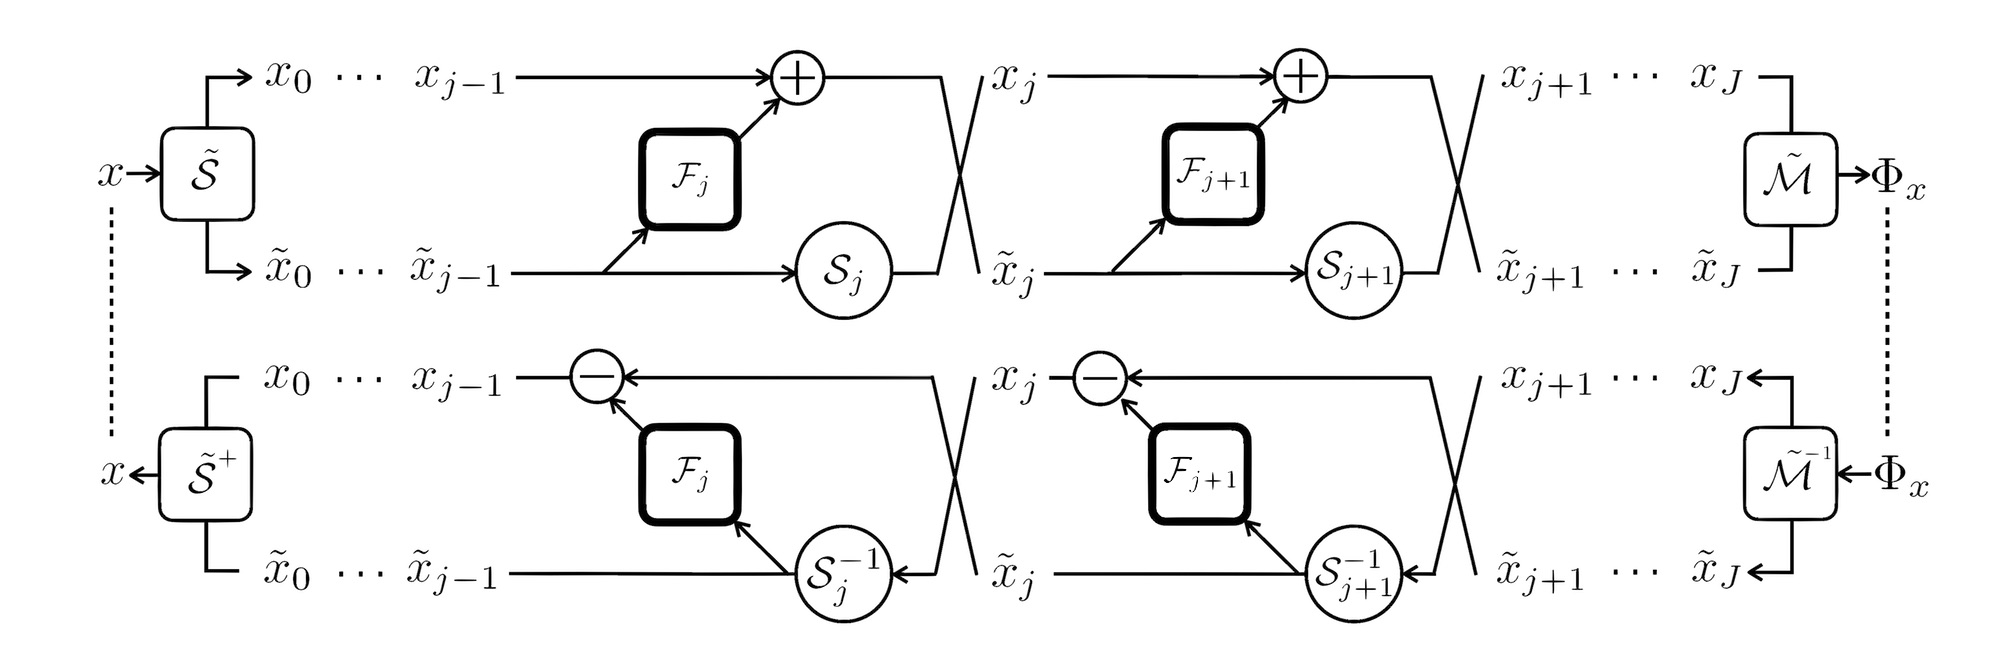
\includegraphics[width=0.95\textwidth]{irevnet-algorithm.jpg}
\caption{The i-RevNet building block, reproduced from \cite{jacobsen2018} (forward pass, top row; inverse,
bottom row). $\tilde{\mathcal S}/\tilde{\mathcal S}^+$ and $\tilde{\mathcal M}/\tilde{\mathcal M}^{-1}$ are
the one-time split/merge operators at the two ends; $\mathcal F_j$ is the (non-invertible, never-inverted)
residual function of \cref{eq:additive-coupling}'s $F$; $\mathcal S_j$ acts on the stream that is not passed
through $\mathcal F_j$ at stage $j$, with its own stated inverse $\mathcal S_j^{-1}$ used on the inverse
path (bottom row). \textbf{What the crossing between consecutive stages means:} at stage $j$ the top stream
$x_{j-1}$ is combined with $\mathcal F_j(\tilde x_{j-1})$ at the $\oplus$ node (this is $y_2=x_2+F(x_1)$ of
\cref{eq:additive-coupling}, with the bottom stream playing $x_1$), while the bottom stream is itself
mapped through $\mathcal S_j$ rather than carried forward unchanged; the crossing lines immediately after
then swap these two results before stage $j+1$, so that the just-updated ($\oplus$-node) stream becomes the
input fed into $\mathcal F_{j+1}$ next, and the $\mathcal S_j$-transformed stream becomes the one updated at
the next $\oplus$. This is the diagrammatic realization of the alternation already described in the main
text above (``successive layers alternate which half plays the role of $x_1$ versus $x_2$''); the only
difference from the bare picture given there is that the carried-forward stream is passed through $\mathcal
S_j$ at each stage rather than left as the identity, which is the source of the possible extra log-det term
this remark flags.}
\label{fig:irevnet-algorithm}
\end{figure}
\end{remark}

\subsection{Injective versus bijective: what the theorem requires, and what each costs to compute}
\label{sec:flow:injective}
Everything so far applies to \emph{any} invertible BB; this subsection is the last purely architectural
one before \cref{sec:flow:implementation} asks which concrete network to use.

\Cref{sec:ng} asks only that $g$ be a diffeomorphism \emph{onto its image}; it does not require the
output dimension to equal the input dimension. An injective embedding into a strictly larger space
satisfies this exactly as well as a dimension-preserving bijection does. Both options require output
dimension at least as large as input dimension -- a bijection meets this with equality, an injective
embedding sits above it -- and this floor is unavoidable for any exactly invertible map; it is not a
special cost of choosing the injective option over the bijective one.

There is, however, a real and separate cost that does distinguish the two, on the computational side of
\cref{eq:flow-nll}. \Cref{sec:flow:coupling} shows that a square (dimension-preserving) map built from
either coupling construction has a triangular Jacobian and is cheap to evaluate -- exactly free
($\det J=1$) for additive coupling regardless of depth \cite{gomez2017}, an $O(n)$ sum for affine
coupling. For a genuinely injective (non-square, dimension-expanding) map, neither of these
constructions, nor the triangular argument behind them, applies: with no square Jacobian, the correct
change-of-volume term is instead the Jacobian-transpose-Jacobian determinant $\det(J^\top J)^{1/2}$ (a
Gram determinant), and computing this -- or even a usable gradient of it -- is a substantially harder
problem that is the subject of ongoing, unresolved research (\emph{Rectangular Flows}, \cite{caterini2021});
current approaches either approximate the term or avoid computing it at all. This is not a limitation of
one particular network; it is a property of dimension-expanding invertible maps in general.

So the dimension-preserving, bijective option is preferable on two independent grounds, not one: it does
not buy accuracy the M1 use case does not need (a point returned to in \cref{sec:flow:implementation}),
and its Jacobian term in \cref{eq:flow-nll} is cheap or free by construction, where the injective
alternative's is an open computational problem. The remainder of this section assumes a bijective,
dimension-preserving BB.

\subsection{Choosing an implementation: i-RevNet versus generative normalizing flows}
\label{sec:flow:implementation}
With ``bijective, coupling-based invertible network'' settled as the architecture family, a separate
question remains: which concrete, ideally pretrained, network to actually use. Three properties matter,
and no candidate available today satisfies all three at once.
\begin{enumerate}[label=(\roman*),leftmargin=2.2em]
\item \label{item:inv} \textbf{Genuinely invertible from raw pixels}, i.e.\ no lossy step anywhere
      between $x$ and the representation used downstream.
\item \label{item:res} \textbf{Pretrained at the target resolution and scale} (full $224\times224$
      general-purpose images, not a narrow domain or a heavily downsampled variant).
\item \label{item:obj} \textbf{Pretrained by an objective aligned with \cref{eq:obs_equiv}}, i.e.\
      density/maximum-likelihood estimation, rather than by a discriminative objective unrelated to
      matching a distribution.
\end{enumerate}

\paragraph{i-RevNet (classification-pretrained).} \cite{jacobsen2018} is a stack of exactly the additive
coupling blocks of \cref{eq:additive-coupling}, pretrained on ImageNet with the standard supervised
classification objective, in a dimension-preserving bijective variant ($\sim$29M parameters, 26.7\%
top-1 error) and a channel-widening injective variant ($\sim$181M parameters, 24.7\% top-1 error,
matching a same-size ResNet-50); \cref{sec:flow:injective}'s argument already favors the bijective one.
It satisfies \labelcref{item:inv} exactly and \labelcref{item:res} directly -- a public, full-resolution
ImageNet-1k checkpoint. It fails \labelcref{item:obj}: nothing in cross-entropy training targets
density estimation. But, per \cref{sec:flow:coupling,sec:flow:injective}, this failure is cheap to have:
because the Jacobian of an additive-coupling block is exactly $1$ regardless of what the block was
trained to do, a classification objective does not make \cref{eq:flow-nll} harder or more expensive to
evaluate -- it can only affect the \emph{geometry} of the learned representation (how conveniently the
surviving, fully-preserved information is arranged for the downstream head and prior to work with), not
whether that information survived (guaranteed by invertibility) or how expensive it is to use.

\paragraph{Off-the-shelf generative normalizing flows (Glow, RealNVP, Residual Flows, \dots).} These are
trained by exact maximum likelihood, so they satisfy \labelcref{item:obj} squarely, and their
square, coupling/1x1-convolution-based architecture satisfies \labelcref{item:inv}. They fail
\labelcref{item:res}: every publicly released checkpoint for this family is at ImageNet $32\times32$ or
$64\times64$ (downsampled) or at CelebA-HQ ($256\times256$, but faces, a much narrower domain), never at
full-resolution general ImageNet. Using one here means retraining from that resolution upward, which
gives up most of what ``pretrained'' was supposed to buy.

\paragraph{Modern large-scale flows (e.g.\ STARFlow \cite{gu2025starflow}).} Recent work has scaled
normalizing flows to real image resolutions with public checkpoints, which looks at first like a
resolution of \labelcref{item:res} for a genuine density-estimation objective. It is not a resolution of
\labelcref{item:inv}, however: this line of work achieves scale specifically by placing the flow inside
the latent space of a standard, lossy autoencoder (an AutoencoderKL-style network) rather than by making
the pixel-to-representation map itself invertible. Adopting it here would reopen exactly the gap
\cref{sec:archB:gap} and \cref{sec:flow:motivation} exist to close, not close it -- the pixel-to-latent
step is the same kind of bottleneck as ResNet-50, only wrapped in a flow further downstream.

\paragraph{Training a bijective coupling flow from scratch on TerraInc-scale data.} The only option that
can satisfy \labelcref{item:inv,item:res,item:obj} simultaneously, since it is fit directly to the target
data and resolution by maximum likelihood, with an architecture chosen for exact invertibility from the
start. The cost is that it gets no benefit from pretraining at all; in that respect it is closer in
spirit to \nameref{sec:archA} (train everything, pay the full cost) than to the frozen-backbone split
this section otherwise describes.

\subsection{Recommendation}
\label{sec:flow:recommendation}
No currently available pretrained network satisfies all three criteria of \cref{sec:flow:implementation}
at once, so the choice is between which criterion to give up. i-RevNet's bijective variant is the
recommended starting point: it is the only candidate that is simultaneously invertible from raw pixels
and available pretrained at the target resolution, and \cref{sec:flow:injective,sec:flow:implementation}
together show that the criterion it fails -- a density-estimation pretraining objective -- is, for this
specific architecture family, a representation-geometry concern rather than a computational one: the
Jacobian term is exactly as cheap under classification pretraining as it would be under any other
objective. That concern is not left untested: it is precisely what the calibration loop already described
in \cref{sec:flow:depth} (held-out negative log-likelihood, plus a separability version of the
linear-probe diagnostic of \cref{app:probe}) is designed to catch. If that calibration shows the
classification-pretrained representation is a poor starting point for the content/style prior to work
with, the fallback is training a bijective coupling flow from scratch (the last option of
\cref{sec:flow:implementation}) -- for the head alone, or, if needed, in place of a pretrained BB
entirely.

\subsection{The training objective, term by term}
\label{sec:flow:objective}
Fixing BB to be the pretrained, frozen i-RevNet bijective backbone of \cref{sec:flow:recommendation}, and
the head to be a second, untrained network built from the coupling-block family of \cref{sec:flow:coupling}
(to be learned from data), the estimation step for one image $x$ from environment $u=(y,t,e)$ proceeds as
follows, replacing \texttt{Trainer.step} of \cref{app:code} term by term.

\begin{enumerate}[label=(\arabic*),leftmargin=2em]
\item \textbf{Encode, deterministically.} Compute $\tilde x=\mathrm{BB}(x)$ (frozen; can be cached once,
      as in \nameref{sec:archB}), then $\hat z=\mathrm{head}^{-1}(\tilde x)$. There is no sampling and no
      \texttt{mu}/\texttt{logvar}: $\hat z$ is one specific value for each $x$.
\item \textbf{Evaluate the prior at $\hat z$, not a KL divergence.} Splitting $\hat z$ into content and
      style blocks as in \cref{eq:split}, compute
      \begin{quote}
      \texttt{cond\_mean=mean\_net(adj\_mat*hat\_z\_c)} and \\
      \texttt{prior\_log\_var=log\_var\_net(domain\_embedding(u))}
      \end{quote}
      exactly as \cref{app:code} already does, and evaluate the ANM/style log-density at the single point
      $\hat z$:
      \begin{equation}
      \log p_{\hat Z}(\hat z\mid u) = \log p\bigl(\hat z_c\bigm|\texttt{cond\_mean},\texttt{prior\_log\_var}\bigr)
      + \sum_{j=1}^{n_s}\log p^{(r)}(\hat z_{s,j}).
      \label{eq:flow-prior-term}
      \end{equation}
      This is the same \texttt{Normal.log\_pdf} computation \cref{app:code} already implements; the only
      change is that it is evaluated once, at a deterministic $\hat z$, rather than compared against an
      approximate posterior.
\item \textbf{Add the encoding map's Jacobian term, via the chain rule.} Writing
      $\Phi=\mathrm{head}^{-1}\circ\mathrm{BB}$ for the full map $x\mapsto\hat z$, the inverse function
      theorem applied to $\mathrm{head}$ gives
      \begin{equation}
      \log\bigl|\det J_\Phi(x)\bigr| = \log\bigl|\det J_{\mathrm{BB}}(x)\bigr|
      - \log\bigl|\det J_{\mathrm{head}}(\hat z)\bigr|.
      \label{eq:flow-jac-split}
      \end{equation}
      Per \cref{sec:flow:coupling,sec:flow:injective}, $\log|\det J_{\mathrm{BB}}(x)|=0$ exactly, since BB
      is built from additive coupling (\cref{eq:additive-coupling}); this term is omitted from the code
      entirely, not computed and found to be zero. $\log|\det J_{\mathrm{head}}(\hat z)|$ is likewise
      exactly $0$ if the head is also pure additive coupling, or the sum of \cref{eq:affine-logdet} over
      the head's constituent layers if the head uses affine coupling instead.
\item \textbf{Assemble the loss.} Combining \cref{eq:flow-nll,eq:flow-prior-term,eq:flow-jac-split} with
      the sparsity penalty of \cref{app:code},
      \begin{equation}
      \mathcal L(x,u) = -\log p_{\hat Z}(\hat z\mid u) - \log\bigl|\det J_{\mathrm{BB}}(x)\bigr|
      + \log\bigl|\det J_{\mathrm{head}}(\hat z)\bigr| + \lambda_{\mathrm{sparse}}\,\ell_{\mathrm{sparse}}(\hat A),
      \label{eq:flow-loss}
      \end{equation}
      where $\ell_{\mathrm{sparse}}(\hat A)$ is \texttt{loss\_sparsity} of \cref{app:code}, computed from
      \texttt{current\_adj\_mat} exactly as before.
\end{enumerate}
\Cref{eq:flow-loss} replaces \texttt{loss\_kl}, \texttt{loss\_rec}, and their weights
\texttt{lambda\_kl}, \texttt{lambda\_rec} outright; \texttt{loss\_sparsity} and \texttt{lambda\_sparse}
carry over unchanged, as does every part of \cref{sec:use}'s prior machinery
(\texttt{mean\_net}, \texttt{log\_var\_net}, \texttt{domain\_embedding}, \texttt{ADJMatrix},
\texttt{find\_sinknodes\_and\_fix}), none of which is aware of, or affected by, how $\hat z$ was produced.

\paragraph{The special case of a purely additive head.} If the head, like BB, uses only additive coupling,
both Jacobian terms of step (3) vanish identically and \cref{eq:flow-loss} reduces to
\begin{equation}
\mathcal L(x,u) = -\log p_{\hat Z}(\hat z\mid u) + \lambda_{\mathrm{sparse}}\,\ell_{\mathrm{sparse}}(\hat A),
\label{eq:flow-loss-additive}
\end{equation}
with no Jacobian computation anywhere in the pipeline: the objective is simply to maximize the prior's
log-density at the transformed point, plus the sparsity penalty -- the same simplification that made the
original NICE construction tractable. The cost is architectural, not computational: a composition of
purely additive-coupling maps can only permute/rearrange density, never locally compress or expand it
(\cref{sec:flow:coupling}), so all of the actual density-shaping needed to match $p_X^{(u)}(x)$ has to
come from the prior side ($\hat A$, \texttt{mean\_net}, \texttt{log\_var\_net}) rather than from $g$
itself. This is not a violation of \cref{thm:ng} -- the theorem only requires \emph{some} diffeomorphism,
and volume-preserving is a valid special case -- but it is a genuine constraint on how flexibly the model
can ultimately fit the observed distribution. If this constraint turns out to bind in practice, the head
(never BB, which is fixed and pretrained) can be switched from additive to affine coupling
(\cref{eq:affine-coupling}), reintroducing the cheap $O(n)$ sum of \cref{eq:affine-logdet} in exchange for
the head being able to locally rescale density rather than merely permute it. \Cref{sec:flow:depth}'s
calibration loop, using held-out $\mathcal L$ from \cref{eq:flow-loss} or \cref{eq:flow-loss-additive} as
appropriate, is the natural place to check whether this constraint is actually binding before paying for
affine coupling. \Cref{sec:flow:headarch} below settles this concretely: for the reasons given there,
affine coupling (not the purely additive case just described) is taken as the default for head, not a
fallback reached for only if a later diagnostic demands it.

\subsection{Head architecture: departing from BB's coupling family}
\label{sec:flow:headarch}
\Cref{sec:flow:split} leaves head's own architecture unspecified beyond ``a genuine flow operating on a
large tensor.'' This subsection fixes it concretely, building on the coupling-layer machinery of
\cref{sec:flow:coupling} but not reusing BB's own block design, for reasons given below.

\paragraph{Head's fixed input/output shape.} The bijective i-RevNet checkpoint of
\cref{sec:flow:recommendation}\footnote{Config \texttt{nBlocks=[6,16,72,6]}, \texttt{nStrides=[2,2,2,2]},
\texttt{nChannels=[24,96,384,1536]}, \texttt{init\_ds=2}, as released for the pretrained model on
\cite{jacobsen2018}'s repository; \texttt{nChannels} denotes channels per coupling stream, not the total.}
applies five factor-2 invertible-squeeze downsamplings in total (\texttt{init\_ds=2} plus the four stage
strides), each quadrupling channels while halving each spatial dimension, taking $3\times224\times224$ to
two streams of $1536$ channels at $7\times7$, i.e.\ a total of $C=3072$ channels at $H=W=7$. As a check,
$C\cdot H\cdot W=3072\cdot49=150528=3\cdot224\cdot224$: exactly the input pixel count, confirming BB is
dimension-preserving as \cref{sec:flow:recommendation} requires. Head therefore never sees a raw image;
its input and output are both this fixed $3072\times7\times7$ tensor, and -- unlike BB -- head needs no
further spatial squeeze stages, since the spatial dimension is already collapsed to $7\times7$: its whole
depth budget goes into channel-mixing and coupling blocks at this one fixed resolution.

\paragraph{Why head should not copy either of BB's own configurations (additive, i-RevNet-style).}
Per \cref{sec:flow:coupling}, additive coupling has $\det J=1$ exactly, so a stack of purely
additive-coupling layers can only permute/rearrange density, never reshape it
(\cref{eq:flow-loss-additive}'s discussion above). BB is fixed to additive coupling, so if head is
\emph{also} purely additive, \emph{no} part of the learned map $g=\mathrm{head}\circ\mathrm{BB}$ can locally
compress or expand volume anywhere; all of the density-shaping needed to match $p_X^{(u)}(x)$ would have to
come entirely from the prior side ($\hat A$, \texttt{mean\_net}, \texttt{log\_var\_net}). Since head is the
only trainable piece of $g$, it should default to affine coupling (\cref{eq:affine-coupling}) from the
start, not treat it as a fallback to reach for only once a diagnostic shows the all-additive case binds.
Separately, i-RevNet's own coupling design (\cref{sec:flow:coupling}, \cref{rem:irevnet-structure}) only
ever swaps two fixed halves of the channels with each other; at $C=3072$ channels this is a restrictive
mixing pattern for a network with no further architectural reason to inherit BB's specific split/merge
design, whose purpose (untangling raw pixels, \cref{sec:flow:depth}) head does not share.

\paragraph{Channel mixing: an invertible \texorpdfstring{$1\times1$}{1x1} convolution between coupling
layers.} \cite{kingma2018glow}'s Glow addresses exactly this restriction by replacing the fixed-half-swap
with a learned, invertible $1\times1$ convolution before each coupling layer, letting every channel mix
with every other channel over depth rather than only its fixed partner half:
\begin{equation}
y_{i,j} = W x_{i,j},\qquad W\in\R^{C\times C}\ \text{invertible},
\label{eq:inv1x1}
\end{equation}
applied identically at every spatial position $(i,j)$ (so it mixes channels only, not space). Its
log-determinant is
\begin{equation}
\log\bigl|\det J\bigr| = H\cdot W_{\mathrm{sp}}\cdot\log\bigl|\det W\bigr|,
\label{eq:inv1x1-logdet}
\end{equation}
(writing $W_{\mathrm{sp}}$ for the spatial width to avoid clashing with the weight matrix $W$), since the
same $C\times C$ map is applied at each of the $H\times W_{\mathrm{sp}}$ positions independently. Computing
$\det W$ directly costs $O(C^3)$ per evaluation, which is non-trivial at $C=3072$ (unlike Glow's own typical
channel counts, a few hundred at most); the standard fix, also from \cite{kingma2018glow}, is to
parameterize $W=PL(U+\mathrm{diag}(s))$ via a fixed permutation $P$ and learned lower/upper-triangular
factors $L,U$, giving $\log|\det W|=\sum_i\log|s_i|$ at $O(C)$ cost. This parameterization should be used
here given head's channel count.

\paragraph{Normalization: ActNorm, not BatchNorm.} The MLPs of \cref{app:code} use \texttt{nn.LayerNorm},
and i-RevNet's own $\mathcal F_j$ blocks (\cref{sec:flow:coupling}) use BatchNorm; neither fits a flow whose
log-likelihood must be exact. BatchNorm's statistics depend on the rest of the batch, in tension with
$\hat z$ being one deterministic value per $x$ (as established in the exchange leading to
\cref{sec:flow:estimation}), and its own log-det contribution is commonly dropped or approximated rather
than computed exactly. \cite{kingma2018glow}'s ActNorm avoids both problems: a per-channel affine transform,
\begin{equation}
y_{i,j} = s\odot x_{i,j} + b,\qquad s,b\in\R^{C},
\label{eq:actnorm}
\end{equation}
with $s,b$ initialized once from the first minibatch (so that the layer's output has zero mean and unit
variance on that batch) and treated as ordinary learned parameters thereafter -- no running statistics, no
batch-dependence at inference. Its log-determinant, by the same per-position argument as
\cref{eq:inv1x1-logdet},
\begin{equation}
\log\bigl|\det J\bigr| = H\cdot W_{\mathrm{sp}}\cdot\sum_{i=1}^{C}\log\bigl|s_i\bigr|,
\label{eq:actnorm-logdet}
\end{equation}
is a plain $O(C)$ sum, of the same cheap form as \cref{eq:affine-logdet}.

\paragraph{One head block, and head's overall composition.} Following \cite{kingma2018glow}'s ``one step of
flow,'' each head block is the composition
\[
\text{ActNorm (\cref{eq:actnorm})} \ \to\ \text{invertible }1\times1\text{ conv (\cref{eq:inv1x1})} \ \to\
\text{affine coupling (\cref{eq:affine-coupling})},
\]
with the coupling layer's own $s(\cdot),t(\cdot)$ realized as small convolutional subnetworks over the
$7\times7$ spatial map (unlike Glow's own multi-scale architecture, which periodically squeezes and splits
off part of the tensor across scales, head applies no further squeeze/split beyond BB's: the whole stack
operates at the one fixed $3072\times7\times7$ shape, per the shape paragraph above). Head's total
log-determinant in \cref{eq:flow-jac-split,eq:flow-loss} is the sum of \cref{eq:inv1x1-logdet,eq:actnorm-logdet} and the coupling term (the affine-coupling analogue of \cref{eq:affine-logdet}) over
all blocks. \Cref{sec:flow:depth}'s 10--20-block guess is a guess about the number of blocks of \emph{this}
composition, not of bare coupling layers as in \cref{sec:flow:coupling} or of BB's own $\mathcal F_j$/
$\mathcal S_j$ design (\cref{rem:irevnet-structure}); head is architecturally closer to Glow than to
i-RevNet, a deliberate departure rather than a smaller or larger copy of BB's own configuration.

\subsection{How deep does the trainable head need to be}
\label{sec:flow:depth}
\Cref{thm:ng} places no requirement on the depth of $g$; any depth that achieves a diffeomorphism onto
its image is equally valid, so this is not a question the identifiability theory answers. Two practical
considerations pull in opposite directions.

Full raw-pixel generative flows (e.g.\ Glow) typically use on the order of a hundred or more coupling
layers, because they must untangle raw pixel-level complexity from scratch. Here that work has already
been done by the frozen backbone, so the head's job is closer to fitting a flow on structured features
than on raw images -- a substantially easier problem, closer in scale to flows used on feature vectors
(single digits to a few tens of coupling blocks) than to full image-generation flows.

Against this, depth in coupling flows is known to matter mainly for numerical conditioning rather than
representational power: a constant number of affine coupling layers can already represent an arbitrary
linear map or permutation exactly, and shallow coupling networks are universal approximators (in
Wasserstein distance) once some ill-conditioning is tolerated \cite{koehler2021}. So there is no
representational floor forcing extra depth; more depth mainly buys better-conditioned training, not
capability this problem specifically requires.

A reasonable starting guess is \textbf{10 to 20 coupling blocks} for the head, to be tuned empirically
rather than derived. Two knobs should be swept together, not decided from first principles: how deep to
cut into the pretrained backbone chosen in \cref{sec:flow:recommendation}, and how many blocks to add on
top. The natural calibration loop reuses tools already in this note: track held-out $\mathcal L$
(\cref{eq:flow-loss}, in place of the held-out ELBO comparison of \cref{app:hnm}) as blocks are added or
the cut point is moved, alongside a version of the linear-probe diagnostic of \cref{app:probe} -- here
asking at which depth content and style are most \emph{separable}, rather than whether they survive at
all, since exact invertibility already guarantees survival by construction.

\subsection{Memory and compute for the trainable head}
\label{sec:flow:memory}
The dominant cost driver is not block count but the fact that an exactly invertible map cannot compress:
a $224\times224\times3$ image is about 150{,}000 elements ($\sim\!588$KB per image in fp32), against the
$\sim\!3072$-dimensional cached embedding of \nameref{sec:archB}. Every accounting below is downstream of
this; it concerns only the trainable head, not the frozen backbone, whose own Jacobian cost was addressed
in \cref{sec:flow:injective,sec:flow:objective}.

\begin{itemize}[leftmargin=1.5em]
\item \textbf{Parameters.} A head of 10 to 20 lightweight convolutional coupling blocks is on the order
      of 20 to 100M parameters ($\sim$100 to 400MB in fp32) -- modest, and not the bottleneck.
\item \textbf{Activation memory, naive autodiff.} Storing every block's activations costs roughly
      batch size $\times$ tensor size $\times$ number of blocks $\times$ an internal expansion factor of
      each coupling block's sub-network ($\sim$2 to 4x). For a batch of 32 and $\sim$15 blocks this lands
      in the range of roughly 1GB to a few GB: workable on a single GPU, but at a far smaller batch size
      than the reference code's default (\texttt{batch\_size=8192} in \texttt{main.py}), which in any
      case was tuned for the tiny tabular toy problem and is not an appropriate default here regardless
      of memory.
\item \textbf{Reversible alternative.} Because every coupling block is invertible by construction, this
      architecture family supports reconstructing each block's input from its output during the backward
      pass instead of caching it (the RevNet/i-RevNet construction), making activation memory
      approximately independent of depth. The published accounting \cite{gomez2017} is a fixed overhead
      of about 33\% more compute (approximately $4N$ unit operations against approximately $3N$ for
      ordinary backprop, for $N$ layers), in exchange for roughly an order-of-magnitude reduction in
      activation memory.
\end{itemize}
At the depth guessed in \cref{sec:flow:depth}, the recommendation is to start \emph{without}
reversibility: it is simpler to implement and debug, and naive-autodiff memory is not yet severe at 10 to
20 blocks. Reversibility is worth adding only if the head grows deeper, or a larger batch is needed than
plain autodiff supports.

\subsection{What this leaves open}
\label{sec:flow:summary}
This section changes only the estimation-method layer of \cref{sec:use}: the map from $X$ to $\hat Z$ and
the loss term that trains it. It leaves \cref{thm:ng}, \cref{as:1,as:2}, and the requirement propositions
of \cref{sec:reqs} untouched, since all of those describe the true generative process rather than the
estimator.

Several items are deferred rather than resolved here. \Cref{sec:flow:objective}'s reduction to
\cref{eq:flow-loss-additive} assumes the head is built from the same additive-coupling family as BB; a
different choice of head (affine coupling, or a different architecture family entirely, e.g.\ one that is
injective rather than bijective) would need the Jacobian term re-derived accordingly, along the lines
already sketched for affine coupling. Whether an all-additive head is expressive enough in practice, or
whether the affine-coupling escape hatch of \cref{sec:flow:objective} is needed, is an empirical question
for the calibration loop of \cref{sec:flow:depth}, not settled here. The recommendation of
\cref{sec:flow:recommendation} also carries its own open item: it rests on the claim that i-RevNet's
classification-pretrained representation is a workable, if unproven, starting point for density
estimation, with the same calibration loop as the check; a negative result there is a live contingency
whose fallback (training a bijective flow from scratch) is named in \cref{sec:flow:recommendation} but
not worked out.

A number of places elsewhere in this note assume the VAE-specific machinery and would need revisiting to
accommodate a flow-based head -- among them, \cref{app:code}'s variable-name mapping (which refers to
encoder/decoder quantities that no longer exist in this form), the phrasing of
\cref{sec:archB,sec:archB:gap} (which should note the injective-backbone case is exempt from the gap they
describe), the pretraining recommendation of \cref{sec:pretrain} (no pretrained self-supervised invertible
backbone on ImageNet is currently available, so an injective/bijective BB is presently obtainable
pretrained only in supervised form, unlike the ResNet-50 case), and the linear-probe diagnostic of
\cref{app:probe} (which would need reframing from ``does information survive'' to ``at which depth is
content/style separability best,'' as noted in \cref{sec:flow:depth}). These are deferred rather than
resolved here.
\newpage

% ---------------------------------------------------------------------
\section{What the i-RevNet reference implementation actually computes}
\label{app:irevnet}

\Cref{sec:flow} proposes using a pretrained, frozen i-RevNet \cite{jacobsen2018} as BB, relying on it being
an exactly invertible, dimension-preserving map with $\log|\det J_{\mathrm{BB}}(x)|=0$. This appendix records,
in the same spirit as \cref{app:code} for the Ng et al.\ reference implementation, what the released
i-RevNet code (\texttt{iRevNet.py}, \texttt{model\_utils.py}, \texttt{ILSVRC\_main.py}) actually computes,
using the authors' own terminology, and derives the Jacobian claim directly from that code rather than from
the architecture family in the abstract.

\subsection{Terminology}
\label{app:irevnet:terms}
The following terms are the authors' own, taken verbatim from the argument help-strings in
\texttt{ILSVRC\_main.py}:
\begin{quote}
\begin{flushleft}
\begin{tabular}{@{}l@{\quad}p{0.75\linewidth}@{}}
\texttt{--nBlocks}  & \emph{`number of blocks per stage'}\\
\texttt{--nStrides} & \emph{`number of strides per stage'}\\
\texttt{--nChannels}& \emph{`number of channels per stage'}\\
\texttt{--init\_ds} & \emph{`initial downsampling'}\\
\texttt{psi} & $\mathcal S_j$, concretely: it's the operator that does ``trade spatial size for channel 
count, losslessly'' -- same job as \texttt{init\_ds}'s squeeze, reused inside every stride-2 block so 
both streams' shapes keep matching $F$'s output after $F$ shrinks the spatial size. It's identity in the 
stride-1 blocks.
\end{tabular}
\end{flushleft}
\end{quote}
\begin{itemize}[leftmargin=1.5em]
\item \textbf{Stage.} One position in the \texttt{nBlocks}/\texttt{nStrides}/\texttt{nChannels} lists.
	  Each stage is a run of blocks at one fixed channel width, with only the first block doing work on 
	  shape.
      \texttt{iRevNet.irevnet\_stack} loops \texttt{zip(nChannels, nBlocks, nStrides)}, one
      (channels, depth, stride) triple per stage, expanded into \texttt{depth} blocks each.
\item \textbf{Block.} One \texttt{irevnet\_block} instance -- the actual coupling layer, in the sense of
      \cref{sec:flow:coupling}'s \cref{eq:additive-coupling}. Nothing coarser than this runs as a single
      computational step.
\item \textbf{Stride.} The help-string (`number of strides per stage') is a little misleading: it is not a
      count, but the one stride value used by a stage. Within a stage, only the \emph{first} block receives
      it (\texttt{strides = [stride] + [1]*(depth-1)} in \texttt{irevnet\_stack}); every other block in the
      stage is hardcoded to stride $1$.
\item \textbf{Channel} (an \texttt{nChannels} entry). The target channel width, per stream (the network
      always carries a pair of streams, \cref{app:irevnet:walkthrough}), for every block in that stage.
\item \textbf{Initial downsampling} (\texttt{init\_ds}). A one-time squeeze applied once, before stage $1$,
      via \texttt{self.init\_psi = psi(init\_ds)}; not itself a stage or a block.
\end{itemize}
\newpage

\subsection{The pretrained checkpoint actually used}
\label{app:irevnet:checkpoint}
The config distributed with the released, pretrained ImageNet checkpoint (the file accompanying
\url{https://drive.google.com/uc?id=1eQtZIpmtVM0-JDv_2nx3xMuGKjA1beLF&export=download} on
\cite{jacobsen2018}'s repository, there named \emph{i-RevNet 301}) is
\begin{quote}
\begin{flushleft}
\begin{quote}
\begin{flushleft}
\texttt{RevNet(nBlocks=[6, 16, 72, 6], nStrides=[2, 2, 2, 2],}\\
\texttt{\phantom{RevNet(}nChannels=[24, 96, 384, 1536],}\\
\texttt{\phantom{RevNet(}nClasses=1000, init\_ds=2, dropout\_rate=0.,}\\
\texttt{\phantom{RevNet(}affineBN=True, in\_shape=[3, 224, 224])}
\end{flushleft}
\end{quote}
\end{flushleft}
\end{quote}
i.e.\ $4$ stages, $100$ total blocks ($6+16+72+6$), reaching top-$1$/top-$5$ accuracy $74.018\%/91.590\%$.
This is the exact command \texttt{README.md} labels ``Train bijective i-RevNet on Imagenet,'' so the
checkpoint is the bijective (dimension-preserving), not the channel-widening injective, variant, despite
being considerably larger than either configuration printed in \cite{jacobsen2018}'s own Table~1 (a $29$M
bijective and a $181$M injective model). An OpenReview discussion thread on the paper independently confirms
the released \texttt{state\_dict} has approximately $119$M parameters -- consistent with this $100$-block
config and inconsistent with the $29$M Table~1 figure -- and separately notes that the released
\texttt{iRevNet.py} uses $3\times3$ kernels throughout each block's bottleneck, where the paper's Section~3.2
describes $1\times1,3\times3,1\times1$; the authors' reply states the released weights are ``a slightly
different version of the network described in the paper for internal reasons'' with unchanged conclusions,
without specifying what else differs. Two things are independently verifiable directly from the code,
however, regardless of that reply: (i) the model is dimension-preserving, checked in
\cref{app:irevnet:walkthrough}; (ii) it is genuinely bijective and not the padded/injective variant, checked
next.

\textbf{Bijective, not injective, confirmed from the channel schedule.} \texttt{irevnet\_block.\_\_init\_\_}
sets \texttt{self.pad = 2*out\_ch - in\_ch}, and only invokes \texttt{injective\_pad} (zero-padding extra
channels) when \texttt{self.pad != 0 and stride == 1}. For a stage's first block (\texttt{stride=2}), this
branch never fires regardless of \texttt{pad}'s value, since \texttt{psi} handles the shape change instead
(\cref{app:irevnet:walkthrough}). For every later, \texttt{stride=1} block in the same stage,
\texttt{irevnet\_stack} sets \texttt{in\_ch = 2 * channel} after each block, so
\texttt{pad = 2*out\_ch - in\_ch = 2*channel - 2*channel = 0} exactly -- \texttt{injective\_pad} never fires
anywhere in this config. The derivation of \cref{app:irevnet:jacobian} assumes this; a different
\texttt{nChannels} schedule that does trigger \texttt{injective\_pad} would need that step re-examined
separately, since it is genuinely dimension-expanding.
\newpage
\subsection{Forward-pass walkthrough}
\label{app:irevnet:walkthrough}
Traced against \texttt{iRevNet.forward} and \texttt{irevnet\_block.forward}, for the checkpoint of
\cref{app:irevnet:checkpoint} and a $3\times224\times224$ input. Everything below carries a \emph{pair} of
streams $(x_1,x_2)$ throughout; this is the coupling split of \cref{sec:flow:coupling}, nothing more.

\paragraph{Step 0: initial downsampling, before any stage.} \texttt{x = self.init\_psi.forward(x)}: 
\texttt{psi(init\_ds=2)} squeezes $3\times224\times224\to12\times112\times112$ (space$\to$channels, factor
$4$), then the result is split in half: $x_1,x_2$ at $6\times112\times112$ each.

\paragraph{Step 1: the four stages.} Only a stage's first block changes shape.
\begin{center}
\begin{tabular}{@{}lclcl@{}}
\toprule
stage & blocks & stride (1st block) & channels/stream & shape in $\to$ out (per stream)\\
\midrule
1 & 6  & 2, then $1\times5$  & 24   & $6\times112\times112\to24\times56\times56$\\
2 & 16 & 2, then $1\times15$ & 96   & $24\times56\times56\to96\times28\times28$\\
3 & 72 & 2, then $1\times71$ & 384  & $96\times28\times28\to384\times14\times14$\\
4 & 6  & 2, then $1\times5$  & 1536 & $384\times14\times14\to1536\times7\times7$\\
\bottomrule
\end{tabular}
\end{center}

\paragraph{Step 2: one block, stride $2$ (a stage's first block).}
\begin{quote}
\begin{flushleft}
\texttt{Fx2 = self.bottleneck\_block(x2)}\\
\texttt{if self.stride == 2:}\\
\texttt{\phantom{if }x1 = self.psi.forward(x1)}\\
\texttt{\phantom{if }x2 = self.psi.forward(x2)}\\
\texttt{y1 = Fx2 + x1}\\
\texttt{return (x2, y1)}
\end{flushleft}
\end{quote}
$F$'s own leading conv has \texttt{stride=stride} built in, so $F$ itself shrinks the spatial size,
computed on the \emph{pre}-\texttt{psi} $x_2$. \texttt{psi} is then applied to \emph{both} streams
afterward, purely to reshape them (space$\to$channels) to match $F$'s new, smaller output shape before the
addition; the table above confirms the reshaped $x_1,x_2$ and $Fx2$ land on the same shape at every stage.

\paragraph{Step 2$'$: one block, stride $1$ (every other block -- $96$ of the $100$ total).} \texttt{psi}
never runs; shapes never change. This is exactly $y_1=x_1,\ y_2=x_2+F(x_1)$ (up to which stream is labelled
$1$ vs.\ $2$), plain additive coupling as in \cref{eq:additive-coupling}, with no extra step.

\paragraph{The \texttt{first} flag.} Only the very first block overall (stage $1$, block $1$) skips its
\texttt{bottleneck\_block}'s leading BatchNorm+ReLU, since the input has just been split from raw pixels and
was never normalized by a prior block.

\paragraph{Kernel sizes.} Every convolution inside \texttt{bottleneck\_block} uses \texttt{kernel\_size=3}
(three $3\times3$ convolutions per block, bottleneck ratio \texttt{mult=4}); per
\cref{app:irevnet:checkpoint} this is not the $1\times1,3\times3,1\times1$ pattern printed in
\cite{jacobsen2018}'s own Section~3.2.

\paragraph{End of the stack.}
\begin{quote}
\begin{flushleft}
\texttt{out\_bij = merge(out[0], out[1])}\ \ \# concat -- $3072\times7\times7$\\
\texttt{out = F.relu(self.bn1(out\_bij))}\ \ \# classifier path only, from here\\
\texttt{out = F.avg\_pool2d(out, self.ds)}\\
\texttt{out = self.linear(out)}\\
\texttt{return out, out\_bij}
\end{flushleft}
\end{quote}
Two separate outputs. \texttt{out} is the $1000$-way ImageNet classifier logits -- not invertible, and not
what \cref{sec:flow} needs. \texttt{out\_bij} is the actual bijective representation, $3072\times7\times7$;
this, not \texttt{out}, is $\tilde x=\mathrm{BB}(x)$ for \cref{sec:flow:split} onward. Using \texttt{out}
instead would silently substitute a lossy, non-invertible quantity for the one the theorem requires.

As a check: $3072\times7\times7=150528=3\times224\times224$, matching the raw pixel count exactly and
confirming dimension-preservation end-to-end, consistent with every row of the table above.

\paragraph{Inverse.} \texttt{iRevNet.inverse} runs the $100$ blocks in reverse order via
\texttt{irevnet\_block.inverse} (subtract $F$; undo \texttt{psi} with \texttt{psi.inverse}, only on the
stride-$2$ blocks), then \texttt{init\_psi.inverse} last -- mirroring Steps~$2\to0$ exactly.

\subsection{The Jacobian of Backbone}
\label{app:irevnet:jacobian}
\textbf{Claim: $\log|\det J_{\mathrm{BB}}(x)|=0$ exactly, for every $x$}, derived from the code above (under
the bijective, \texttt{injective\_pad}-free config of \cref{app:irevnet:checkpoint}), not merely asserted
from the additive-coupling architecture family in the abstract.

\paragraph{Step 1: every \texttt{psi} call has $|\det|=1$.} \texttt{psi.forward}/\texttt{.inverse}
(\texttt{model\_utils.py}) are pure \texttt{reshape}+\texttt{permute}: every output entry equals exactly one
input entry, relocated, with no arithmetic combination of values. As a linear map on flattened coordinates
this is a permutation matrix, so $\det=\pm1$ regardless of input. This covers \texttt{init\_psi} (once, Step
0) and every per-block \texttt{psi} call (once per stage, in that stage's stride-$2$ block, applied to
\emph{both} streams).

\paragraph{Step 2: every block has $|\det|=1$ -- including the part that is not obvious in advance.} The
code's actual output order is \texttt{(x2, y1)} with \texttt{y1 = Fx2 + x1}, i.e.\ the map
$(x_1,x_2)\mapsto(x_2,\ x_1+F(x_2))$, whose Jacobian in block form is
\begin{equation}
J=\begin{pmatrix}0 & I\\ I & \partial F/\partial x_2\end{pmatrix}.
\label{eq:irn-block-jac}
\end{equation}
Swapping the two row-blocks gives $\begin{pmatrix}I & \partial F/\partial x_2\\ 0 & I\end{pmatrix}$ --
upper-triangular, identity diagonal, $\det=1$ -- and a row-block swap only changes the sign of the
determinant, never its magnitude. So $|\det J_{\text{block}}|=1$ exactly, and 
$\partial F/\partial x_2$ -- everything the BatchNorm/ReLU/conv stack inside \linebreak
\texttt{bottleneck\_block} computes -- cancels out of the
determinant entirely; this is also why $F$ itself never needs to be invertible. For a stride-$2$ block, 
this structure composes with the (Step~1) \texttt{psi} application on both streams; a product of two
unit-magnitude determinants is itself unit-magnitude.

\paragraph{Step 3: the final \texttt{merge}.} \texttt{out\_bij = merge(out[0], out[1])} is
\texttt{torch.cat} -- again a pure reshape, $|\det|=1$.

\paragraph{Step 4: compose across the whole network.} Log-determinant of a composition is the sum of the
pieces' log-determinants:
\begin{equation}
\log\bigl|\det J_{\mathrm{BB}}(x)\bigr| = \underbrace{0}_{\texttt{init\_psi}} \!\!+
\sum_{\substack{\text{100}\\\text{blocks}}} \underbrace{0}_{\text{each block}} \!\!+\; 
\underbrace{0}_{\texttt{merge}} \;=\; 0,
\label{eq:irn-total-jac}
\end{equation}
identically in $x$. \Cref{eq:irn-total-jac} is what \cref{eq:flow-jac-split,eq:flow-loss} use as
$\log|\det J_{\mathrm{BB}}(x)|=0$; \cref{rem:irevnet-structure}'s open question about whether the per-
stage $\mathcal S_j$ operator (identified there as \texttt{psi}) might carry its own non-trivial log-det 
term is resolved by Step~1 above: it does not, in this implementation.

\paragraph{Scope of this derivation.} It assumes the \texttt{injective\_pad}-free channel schedule 
confirmed
in \cref{app:irevnet:checkpoint} for the actual released checkpoint. A different \texttt{nChannels}
configuration for which \texttt{pad != 0} at some \texttt{stride=1} block would introduce a genuinely
dimension-expanding padding step there, and \cref{eq:irn-total-jac} would not apply to that variant 
without separately accounting for it.

\newpage

% =====================================================================
\begin{thebibliography}{15}
\addcontentsline{toc}{section}{References}

\bibitem{caterini2021}
A.L.~Caterini, G.~Loaiza-Ganem, G.~Pleiss, and J.P.~Cunningham.
\newblock Rectangular Flows for Manifold Learning.
\newblock \url{https://arxiv.org/abs/2106.01413}

\bibitem{gomez2017}
A.N.~Gomez, M.~Ren, R.~Urtasun, and R.B.~Grosse.
\newblock The Reversible Residual Network: Backpropagation Without Storing Activations.
\newblock \url{https://arxiv.org/abs/1707.04585}

\bibitem{gu2025starflow}
J.~Gu, T.~Chen, D.~Berthelot, H.~Zheng, Y.~Wang, R.~Zhang, L.~Dinh, M.A.~Bautista, J.~Susskind, and S.~Zhai.
\newblock STARFlow: Scaling Latent Normalizing Flows for High-resolution Image Synthesis.
\newblock \url{https://arxiv.org/abs/2506.06276}

\bibitem{hyvarinen1999}
A.~Hyv{\"a}rinen and P.~Pajunen.
\newblock Nonlinear independent component analysis: existence and uniqueness results.
\newblock \emph{Neural Networks}, 12(3):429--439, 1999.

\bibitem{jacobsen2018}
J.-H.~Jacobsen, A.~Smeulders, and E.~Oyallon.
\newblock \textit{i}-RevNet: Deep Invertible Networks.
\newblock \url{https://arxiv.org/abs/1802.07088}
\newblock Implemented at \url{https://github.com/jhjacobsen/pytorch-i-revnet}

\bibitem{khemakhem2020}
I.~Khemakhem, D.~P. Kingma, R.~P. Monti, and A.~Hyv{\"a}rinen.
\newblock Variational autoencoders and nonlinear {ICA}: a unifying framework.
\newblock In \emph{Proc.\ AISTATS}, PMLR 108, 2020, pp.~2207--2217.
\newblock \url{https://proceedings.mlr.press/v108/khemakhem20a.html}

\bibitem{kingma2018glow}
D.~P.~Kingma and P.~Dhariwal.
\newblock Glow: Generative Flow with Invertible 1x1 Convolutions.
\newblock In \emph{Proc.\ NeurIPS}, 2018.
\newblock \url{https://arxiv.org/abs/1807.03039}

\bibitem{aekl}
D.P.~Kngma and M.Welling
\newblock Auto-Encoding Variational Bayes.
\newblock \url{https://arxiv.org/abs/1312.6114}
\newblock Implemented at \url{https://huggingface.co/docs/diffusers/en/api/models/autoencoderkl}

\bibitem{koehler2021}
F.~Koehler, V.~Mehta, and A.~Risteski.
\newblock Representational aspects of depth and conditioning in normalizing flows.
\newblock \url{https://arxiv.org/abs/2010.01155}

\bibitem{kong2022}
L.~Kong, S.~Xie, W.~Yao, Y.~Zheng, G.~Chen, P.~Stojanov, V.~Akinwande, and K.~Zhang.
\newblock Partial disentanglement for domain adaptation.
\newblock In \emph{Proc.\ ICML}, PMLR 162, 2022, pp.~11455--11472.
\newblock \url{https://proceedings.mlr.press/v162/kong22a.html}

\bibitem{leng2025repae}
X.~Leng, J.~Singh, Y.~Hou, Z.~Xing, S.~Xie, L.~Zheng
\newblock REPA-E: Unlocking VAE for End-to-End Tuning with Latent Diffusion Transformers
\newblock \url{https://arxiv.org/abs/2504.10483}
\newblock Implemented at \url{https://github.com/End2End-Diffusion/REPA-E}

\bibitem{nash1956}
J.~Nash 
\newblock The imbedding problem for Riemannian manifolds. 
\newblock Annals of Mathematics, 63(1) -20–63, 1956. ISSN 0003486X. 
\newblock \url{http://www.jstor.org/stable/1969989}

\bibitem{ng2025}
I.~Ng, S.~Xie, X.~Dong, P.~Spirtes, and K.~Zhang.
\newblock Causal representation learning from general environments under nonparametric mixing.
\newblock In \emph{Proc.\ AISTATS}, PMLR 258, 2025 (revised version: arXiv:2604.23800).
\newblock \url{https://arxiv.org/abs/2604.23800}

\bibitem{ngimpl}
I.~Ng, S.~Xie, X.~Dong, P.~Spirtes, and K.~Zhang.
\newblock Implementation of ``Causal representation learning from general environments under nonparametric mixing.''
\newblock \url{https://github.com/ignavierng/crl-general-environments}

\bibitem{rolland2022}
P.~Rolland, V.~Cevher, M.~Kleindessner, C.~Russell, D.~Janzing, B.~Sch{\"o}lkopf, and F.~Locatello.
\newblock Score matching enables causal discovery of nonlinear additive noise models.
\newblock In \emph{Proc.\ ICML}, 2022.

\bibitem{zhan2026blae}
Q.~Zhan, Z.~Zhou, Z.~Wang, Q.~Long, and L.~Shen
\newblock Bi-Lipschitz Autoencoder With Injectivity Guarantee
\newblock \url{https://arxiv.org/abs/2604.06701}
\newblock Implemented at \url{https://github.com/End2End-Diffusion/REPA-E}
\newblock Implemented at \url{https://github.com/qipengz/BLAE}


\bibitem{zhang2024}
K.~Zhang, S.~Xie, I.~Ng, and Y.~Zheng.
\newblock Causal representation learning from multiple distributions: a general setting.
\newblock In \emph{Proc.\ ICML}, 2024 (arXiv:2402.05052).
\newblock \url{https://arxiv.org/abs/2402.05052}

\end{thebibliography}

\end{document}
